\documentclass{report}
\usepackage[utf8]{inputenc}
\usepackage{physics}
\usepackage{amsmath,amsfonts,amsthm,bm, amssymb}
\usepackage[a4paper]{geometry}
\usepackage{tikz}
\usepackage{graphicx}
\usepackage{subcaption}
\usepackage{tabulary}
\usepackage[acronym,toc]{glossaries}
\usepackage[sorting=none, backend=biber, citestyle=numeric-comp]{biblatex}
\usepackage{wrapfig}
\usepackage[xetex]{hyperref}
\usepackage[all]{hypcap}

\hypersetup{
	colorlinks=true,
	linkcolor=blue,
	filecolor=blue,      
	urlcolor=blue,
	bookmarks=true,
	citecolor=blue,
	pdfauthor=Hugo Levy-Falk
}

\title{Imperial College London\\MSc in Optics and Photonics summer project\\Hybrid chiral lasers}
\author{Hugo Levy-Falk\\Supervisor : Prof. Martin McCall}
\date{2020}

\addbibresource{biblio.bib}

\newacronym{cwt}{CWT}{Coupled Wave Theory}

\newenvironment{acknowledgements}%
{\cleardoublepage\thispagestyle{empty}\null\vfill\begin{center}%
		\bfseries Acknowledgements\end{center}}%
{\vfill\null}

\usetikzlibrary{decorations.pathreplacing}

\begin{document}
	
\maketitle

\begin{abstract}
	
	This document reports a study on hybrid chiral lasers. It extends the coupled wave theory used by \citename{topf_modes_2014} to develop a simple chiral cavity laser model. Three cavity designs are modelled: a simple cavity with a twist defect at the centre, a hybrid cavity with a gain medium surrounded by two reflectors of opposite handedness and a cavity mixing the two previous designs. It is shown the latter design corresponds to a tunable chiral laser offering almost pure circularly polarised output.

\end{abstract}

\begin{acknowledgements}
	I would like to thank Martin McCall, whose pieces of advice have always been really helpful, for offering me the opportunity to work on this topic while allowing me to look in any direction I thought useful. This has been a great occasion for me to grow a much deeper understanding of photonic structures and their behaviours.
	
	I also thank Nathan Alglave, who introduced me to Blender and advised me on how to use it. His pieces of advice are the reason I was able to produce nice representations of chiral cavity such as the ones in figure \ref{fig:cavities_blender}.
	
	I am also grateful towards my friends who accepted to proof-read my clumsy english to make this report somewhat understandable.
	
	Finally I would like to thank Mathworks, the company editing the MATLAB language, for their poor taste in programming language designs. This helped me remember how much I prefer working with the Julia programming language.
\end{acknowledgements}

\tableofcontents
\listoffigures

\chapter{Introduction}

Polarisation is an important property of light, arising from Maxwell equations\cite{weir_optical_2019}. It refers to the direction of oscillation of the electromagnetic field. Even naked human eyes can display some sensitivity to the state of polarisation of light\cite{le_floch_polarisation_2010}. However, the perception of polarisation is much more developed within animal kingdom. This led to the development of advanced characterization techniques of animal species such as beetles\cite{carter_variation_2016}. Fine control over polarisation and polarised emitters also have important applications \textit{e.g.} in quantum information technologies\cite{bennett_quantum_2014} and for commercial RealD 3D digital
stereoscopic projection technologies\cite{mendiburu_chapter_2009}.

Chiral structures are a highly studied area\cites{belyakova_optical_2011}{harutyunyan_optical_2007}{mccall_simplified_2009}{mccall_properties_2009} as this kind a photonic structure allows for unusual optical properties. Among them is the ability to produce circularly polarised laser outputs when pumped\cites{topf_modes_2014}{kopp_twist_2002}{oldano_comment_2004}. Chiral structures are often associated whit liquid-crystals media. Those are versatile materials that allow producing laser outputs when pumped \cites{coles_liquid-crystal_2010}{gardiner_paintable_2011}. Such lasers can also be arranged in arrays\cite{hands_two-dimensional_2008}.

This study draws out the work of \textcite{topf_modes_2014}. It extends coupled wave theory to have analytical expressions for left-handed media and every possible interfaces between chiral and isotropic media. Previous results on chiral media are reproduced and three designs of chiral lasers are proposed to produce circularly polarised outputs.

The first chapter of the report introduces the two theories used and the extensions derived during this study. It also offers a short review of past results on chiral media and presents the cavity designs modelled.

The second chapter gives the methods used to characterise the cavities: the polarisation output as well as the light intensity distribution within the media for every identified laser mode.

The third chapter brings the results obtained for each of the cavities, in terms of reflectivity when it makes sense and of laser output. The cavity proposed by \textcite{topf_modes_2014} is reproduced and similar results to theirs are reported. The three other cavities present interesting properties in term of tunability and purity of output.

Finally a conclusion is drawn on this study and more specifically the cavity designs allowing circular polarised outputs. Some future prospects on chiral lasers are outlined.

Several comparisons between the two theories used are available in appendix, as well as a list of the files used to make the figures of this report in appendix \ref{chap:sourcecode}. The files are hosted at \url{https://github.com/Klafyvel/Hybrid-Chiral-Lasers}.
\chapter{Background}
This chapter aims to bring the definitions, fundamental theory as well as a review of related experimental work on chiral media in optics. A presentation of both an exact (Oseen method) and an approximate (Coupled Wave Theory) theory, derived by \textcite{mccall_simplified_2009} is given. The approximate theory is extended to provide an expression accounting for rotation of the medium along the propagation axis, as well as a treatment of all kind of interfaces between chiral and isotropic media. 
\section{Definitions and notations}

\subsection{Description of the medium, Maxwell equations and electromagnetic field}

This study focuses on studying the propagation of plane waves in media presenting an anisotropic permittivity $\epsilon_0\bm{\epsilon}$, with $\bm{\epsilon}$ given in equation \ref{eq:epsilon}.
\begin{equation}
\bm{\epsilon} = \begin{pmatrix}\bm{R}^{-1}(z)\cdot\begin{pmatrix}
\epsilon_a & 0\\
0 & \epsilon_b\\
\end{pmatrix}\cdot\bm{R}(pz) & \begin{matrix}
0\\0
\end{matrix}\\
\begin{matrix}
0 & 0
\end{matrix} & \epsilon_c
\end{pmatrix}
\label{eq:epsilon}
\end{equation}
%
Where $\bm{R}$ is a rotation matrix. Rotations in the plane, of angle $\varphi$, are described by the orthogonal matrix $\bm{R}(z)$ in equation \ref{eq:rotation}. $z$ is the position in the medium, $p$ the periodicity of the rotation, $\psi$ the phase of the rotation at the origin and $\epsilon_{a,b,c}$ are relative permittivities. The medium can therefore be understood as a birefringent medium whose axes are rotated in the $x,y$ plane for each position on the $z$ axis. Experimental realisations of such media are presented in section \ref{sec:experimental_work}.

\begin{equation}
\bm{R}(z) = \begin{pmatrix}
\cos(pz+\psi) & -\sin(pz+\psi)\\
\sin(pz+\psi) & \cos(pz+\psi)
\end{pmatrix} \label{eq:rotation}
\end{equation}

This allows to write Maxwell-Faraday and Maxwell-Ampère laws in a dielectric for $\bm{E}$ and $\bm{B}$ as in equations \ref{eq:faraday} and \ref{eq:ampere}.
\begin{eqnarray}
\nabla \times\bm{E} &=& -\mu_0\pdv{\bm{H}}{t}\label{eq:faraday}\\
\nabla \times\bm{H} &=& \epsilon_0\bm{\epsilon}\cdot\pdv{\bm{E}}{t}\label{eq:ampere}
\end{eqnarray}
%
In order to study the effects of the anisotropy, we consider only the derivative against $z$ of the cross-products, leading to equations \ref{eq:de_h} and \ref{eq:dh_e}.
\begin{eqnarray}
\bm{\hat{z}}\dv{z}\times\bm{E}_\perp &=& ik_0\bm{H}'_\perp \label{eq:de_h}\\
\bm{\hat{z}}\dv{z}\times\bm{H}'_\perp &=& -ik_0\bm{\epsilon}_\perp\cdot\bm{E}_\perp \label{eq:dh_e}
\end{eqnarray}
%
Where the notation $\perp$ is used to refer to the sub-vector of the field in $x,y$ plane or the components of the sub-matrices dealing with components of the field in that plane\footnote{As the study focuses on the field in the $x,y$ plane, the $\perp$ symbol is often omitted.}. We also make use of a reduced $\bm{H}$ field, $\bm{H'}$, defined in equation \ref{eq:hp}. 
\begin{eqnarray}
\bm{H}' &=& \left(\frac{\mu_0}{\epsilon_0}\right)^{1/2}\bm{H} \label{eq:hp}
\end{eqnarray}

\subsection{Handedness}
\label{seq:handedness}
The chosen definition used for handedness of polarization is that the field is said to be left-handed (respectively right-handed) if the helix it describes is left-handed (respectively right-handed). This definition does not depend on the direction of propagation. Figure \ref{fig:handedness} illustrates the two possible handedness.

Formally, this means that in equation \ref{eq:epsilon}, a right-handed medium would have a positive value of $p$ while a left-handed one would have a negative one.

\begin{figure}
	\centering
	\begin{subfigure}{0.49\textwidth}
		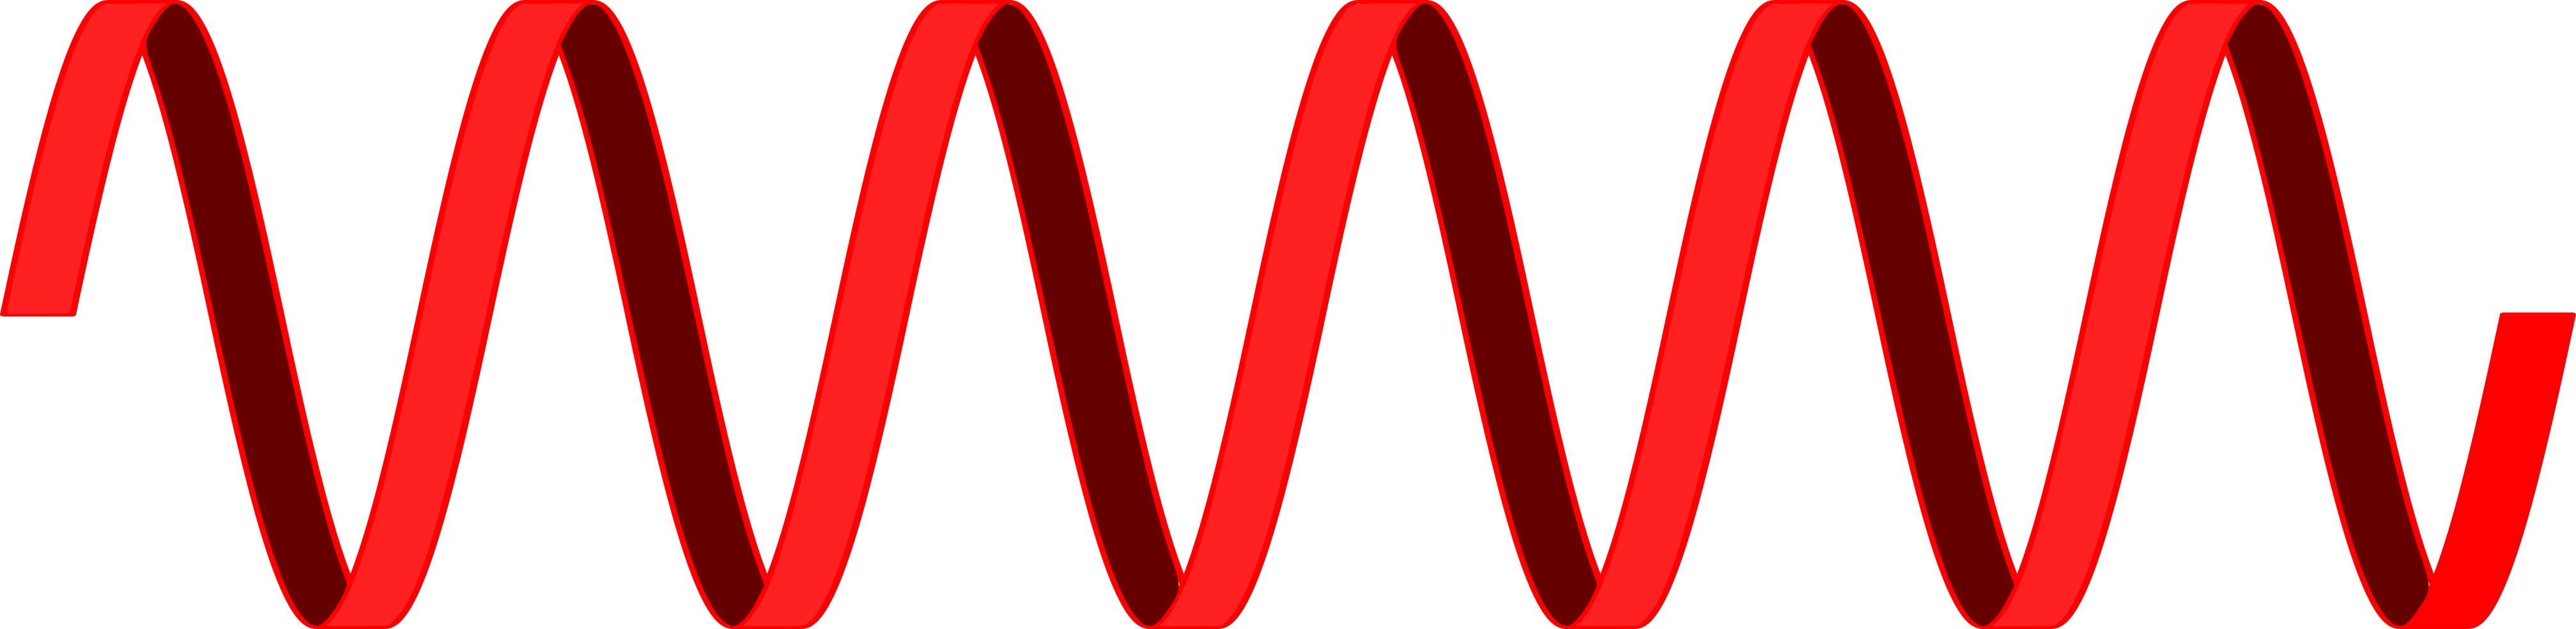
\includegraphics[width=\textwidth]{images/left_handed.png}
		\caption{}
		\label{fig:left_handed}
	\end{subfigure}
	\begin{subfigure}{0.49\textwidth}
		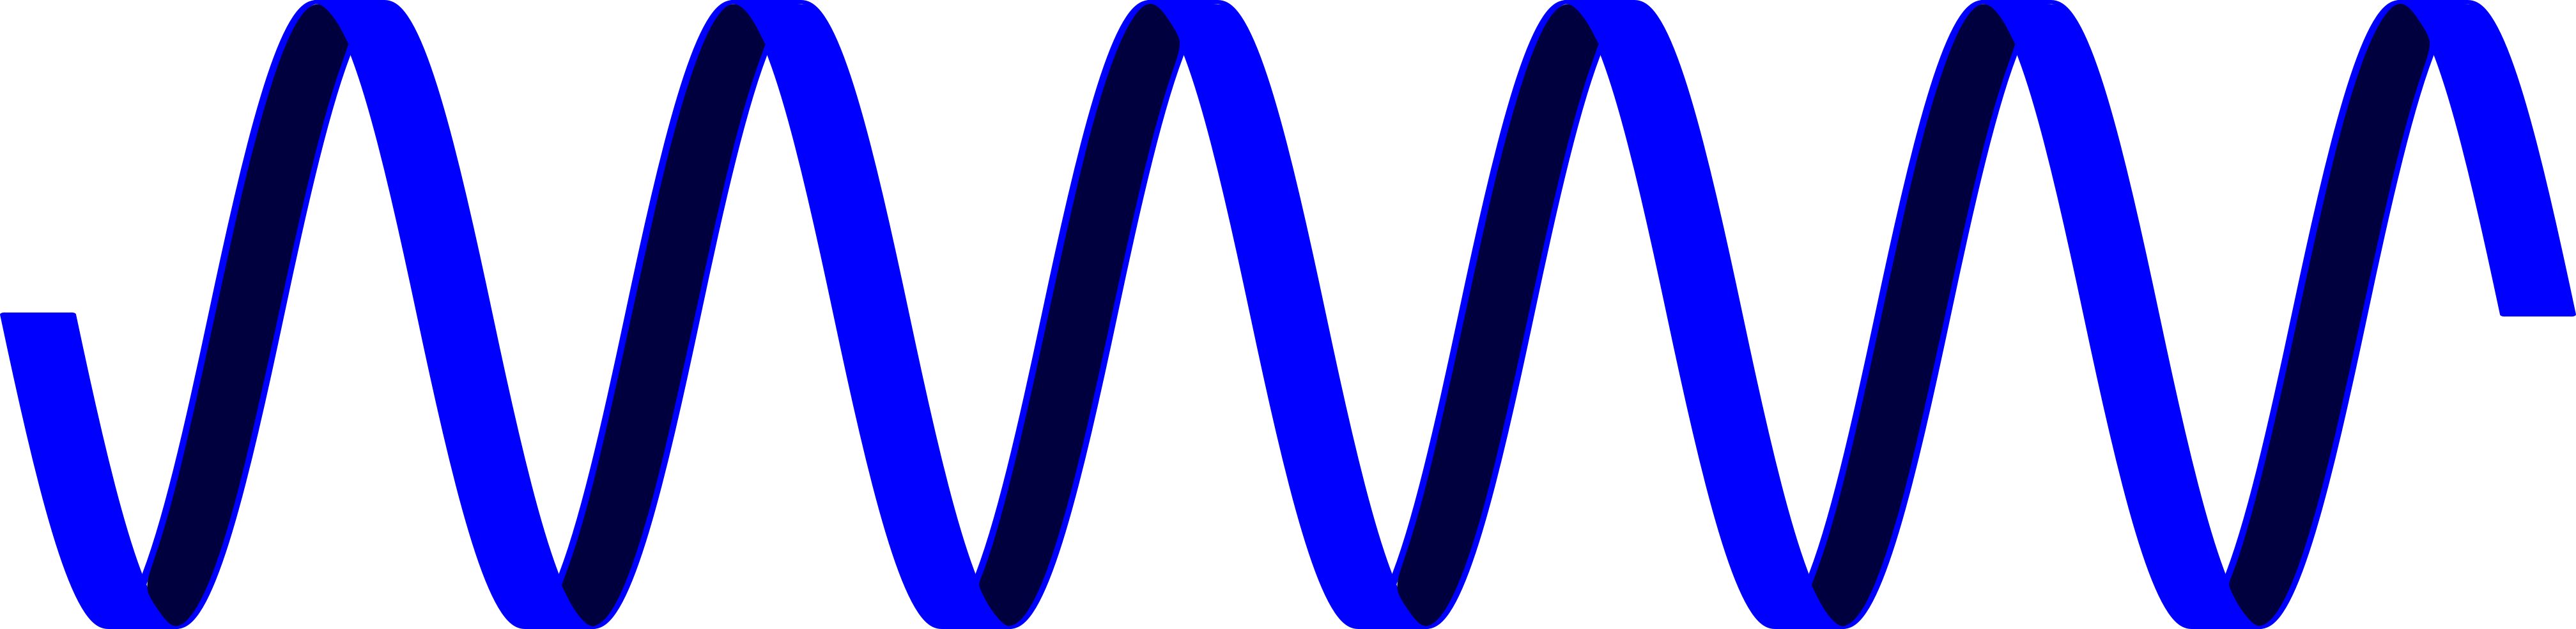
\includegraphics[width=\textwidth]{images/right_handed.png}
		\caption{}
		\label{fig:right_handed}
	\end{subfigure}
	\caption[Helix handedness]{\ref{fig:left_handed} Left handed helix. \ref{fig:right_handed} Right handed helix.}
	\label{fig:handedness}
\end{figure}

\subsection{Transfer matrices and bases for the field}

The cavity configurations explored in this report are described with the help of transfer matrices. Three bases are used to describe the field.
\begin{description}
	\item[Electromagnetic basis] The field is represented under the form $\left[E_x, E_y, H'_x, H'_y\right]^T$. Continuity of tangential components of the field allows to directly multiply two matrices describing two media to get the matrix describing the two media combined. However, this representation does not give a direct image of the components of the field propagating forward or backwards in the medium.
	\item[Cartesian basis] The field is written in the form $\left[E_x^+, E_y^+, E_x^-, E_y^-\right]^T$. This base allows to directly represent the field direction. However, the media studied induce circularly polarised field. This field is mainly used as a transition between electromagnetic and circular bases.
	\item[Circular basis] This is the basis of main interest for this study. The two main vectors are $\bm{e_1}$ and $\bm{e_2}$, given by equations \ref{eq:e1} and \ref{eq:e2}. The field is written $\left[E_L^+, E_R^+, E_L^-, E_R^-\right]^T$.
	\begin{eqnarray}
	\bm{e_1} &=& \frac{1}{\sqrt{2}}\begin{bmatrix}
	1\\i
	\end{bmatrix}\label{eq:e1}\\
	\bm{e_2} &=& \frac{1}{\sqrt{2}}\begin{bmatrix}
	1\\-i
	\end{bmatrix}\label{eq:e2}
	\end{eqnarray}
\end{description}
%
It is worth to note that $\bm{E}$ can be retrieved easily, independently from the medium \textit{via} equation \ref{eq:E}.
\begin{equation}
\bm{E} = \underbrace{E_L^+\bm{e_1}+E_R^+\bm{e_2}}_{=\begin{bmatrix}E_x^+\\E_y^+\end{bmatrix}}+\underbrace{E_L^-\bm{e_2}+E_R^-\bm{e_1}}_{=\begin{bmatrix}E_x^-\\E_y^-\end{bmatrix}}\label{eq:E}
\end{equation}
%
$\bm{H'}$ however is more difficult to calculate, and depends on the medium and the method used to simulate it.

\subsection{Partial inverse and reflection coefficients}
\label{sec:reflection}
One interesting feature of transfer matrices is that they allow the calculation of reflectivity quite easily, allowing to compare reflectivities with known results\cite{mccall_simplified_2009}. This subsection introduces a systematic way of expressing those coefficients, using partial inverses of matrices\cite{noauthor_partial_2020}.

If a matrix $\bm{M}$ links a state of light 0 to a state of light 1 (\textit{e.g.} for an interface or the propagation through a slab of chiral medium), \textit{i.e.} $\left[E_a, E_b, E_c, E_d\right]^T_{1} = \bm{M}\left[E_a, E_b, E_c, E_d\right]^T_{0}$, $\bm{M}$ can be rewritten by blocks
\begin{equation}
\begin{bmatrix}
E_a^+ \\
E_b^+ \\
E_a^- \\
E_b^- \\
\end{bmatrix}_{1} = \begin{pmatrix}
\bm{M_{11}} & \bm{M_{12}}\\
\bm{M_{21}} & \bm{M_{22}}\\
\end{pmatrix}\begin{bmatrix}
E_a^+ \\
E_b^+ \\
E_a^- \\
E_b^- \\
\end{bmatrix}_{0}
\end{equation}
By defining the partial inverse of $\bm{M}$, $\text{inv}_1(\bm{M})$, as
\begin{equation}
\text{inv}_1(\bm{M}) = \begin{pmatrix}
\bm{M_{11}}^{-1} & -\bm{M_{11}}^{-1}\bm{M_{12}}\\
\bm{M_{21}}\bm{M_{11}}^{-1} & \bm{M_{22}}-\bm{M_{21}}\bm{M_{11}}^{-1}\bm{M_{12}}\\
\end{pmatrix}
\end{equation}
We get
\begin{equation}
\begin{bmatrix}
E_{a,1}^+ \\
E_{b,1}^+ \\
E_{a,0}^- \\
E_{b,0}^- \\
\end{bmatrix} = \left(\text{inv}_1(\bm{M})\right)^{-1}\begin{bmatrix}
E_{a,0}^+ \\
E_{b,0}^+ \\
E_{a,1}^- \\
E_{b,1}^- \\
\end{bmatrix}\label{eq:pinv}
\end{equation}
Thus by knowing the boundary conditions $[E_{a,0}^+, E_{b,0}^+, E_{a,1}^-, E_{b,1}^-]^T$, it is possible to know the reflected and transmitted field $[E_{a,1}^+,E_{b,1}^+,E_{a,0}^-,E_{a,0}^-]^T$. 

By setting $[E_{a,1}^-, E_{b,1}^-] = \bm{0}$ in equation \ref{eq:pinv}\footnote{This no light is shone from the other side of the slab}, it is straightforward to see that the amplitude reflection and transmission coefficients associated to $\bm{M}$ are given by the first two columns of $\left(\text{inv}_1(\bm{M})\right)^{-1}$.
\begin{equation}
\left(\text{inv}_1(\bm{M})\right)^{-1} = \begin{pmatrix}
t_{aa} & t_{ab} & \ldots \\
t_{ba} & t_{bb} & \ldots \\
r_{aa} & r_{ab} & \ldots \\
r_{ba} & r_{bb} &  \ldots\\
\end{pmatrix}
\end{equation}
%
This allows to express directly the reflection and transmission coefficients.

\begin{eqnarray}
\begin{pmatrix}
t_{aa} & t_{ab} \\
t_{ba} & t_{bb}
\end{pmatrix} &=& \bm{M_{11}} - \bm{M_{12}}\bm{M_{22}}^{-1}\bm{M_{21}} \label{eq:transmission}\\
\begin{pmatrix}
r_{aa} & r_{ab} \\
r_{ba} & r_{bb}
\end{pmatrix} &=& -\bm{M_{22}}^{-1}\bm{M_{21}}\label{eq:reflection}
\end{eqnarray}

\subsection{Energy conservation}

From the reflection coefficients, it is possible to check energy conservation in the medium. Three criteria can be distinguished\cite{mccall_properties_2009}.  Expressing reflection coefficients in an arbitrary basis as in section \ref{sec:reflection}, equations \ref{eq:energyconservationa} and \ref{eq:energyconservationb} correspond to energy conservation for light incident to the medium with polarisation states $a$ and $b$ respectively. Equation \ref{eq:energyconservationredistribution} accounts for redistribution of energy between polarization states $a$ and $b$. $n1$ and $n2$ are the refractive indices of the isotropic media before and after the chiral medium.

\begin{eqnarray}
\abs{r_{aa}}^2+\abs{r_{ba}}^2+\left(\frac{n_2}{n_1}\right)(\abs{t_{aa}}^2+\abs{t_{ba}}^2)-1&=&0\label{eq:energyconservationa}\\
\abs{r_{ab}}^2+\abs{r_{bb}}^2+\left(\frac{n_2}{n_1}\right)(\abs{t_{ab}}^2+\abs{t_{bb}}^2)-1&=&0\label{eq:energyconservationb}\\
r_{aa}r_{ab}^*+r_{ba}r_{bb}^*+\left(\frac{n_2}{n_1}\right)(t_{aa}t_{ab}^*+t_{ba}t_{bb}^*) &=& 0 \label{eq:energyconservationredistribution}
\end{eqnarray}
\section{Oseen transformation}

The Oseen transformation allows to give an exact solution for the electromagnetic fields in a chiral medium, although it does not yield an explicit form of the propagation matrix.

\subsection{Derivation of transfer matrix equation}

The main idea behind this method is to use a well-chosen change of basis, named "the Oseen transformation", described by equation \ref{eq:oseen_transformation}.

\begin{eqnarray}
\bm{e}(z) = \bm{R}^{-1}(z)\cdot\bm{E}_\perp(z) &,& \bm{h}(z) = \bm{R}^{-1}(z)\cdot\bm{H}'_\perp(z) \label{eq:oseen_transformation}
\end{eqnarray}
%
By rewriting equations \ref{eq:de_h} and \ref{eq:dh_e} as follow:
\begin{eqnarray}
\dv{z}\bm{E}_\perp = ik_0\begin{pmatrix}
0 & 1\\-1 & 0
\end{pmatrix}\bm{H}'_\perp&,&
\dv{z}\bm{H}'_\perp = -ik_0\begin{pmatrix}
0 & 1\\-1 & 0
\end{pmatrix}\bm{\epsilon}\bm{E}_\perp
\end{eqnarray}
%
and noting that $\dv{z}\bm{R}^{-1} = p\begin{pmatrix}
0 & 1 \\ -1 & 0
\end{pmatrix} \bm{R}^{-1}$, these two intermediate quantities must therefore verify equation \ref{eq:oseen_intermediate}.

\begin{eqnarray}
\dv{z}\begin{bmatrix}
e_x\\e_y\\h_x\\h_y
\end{bmatrix} = i\underbrace{\begin{pmatrix}
	0 & -ip & 0 & k_0\\
	ip & 0 & -k_0 & 0\\
	0 & -k_0\epsilon_b & 0 & -ip\\
	k_0\epsilon_a & 0 & ip & 0\\
	\end{pmatrix}}_{=\bm{G}}\begin{bmatrix}
e_x\\e_y\\h_x\\h_y
\end{bmatrix} \label{eq:oseen_intermediate}
\end{eqnarray}
%
Remarkably, equation \ref{eq:oseen_intermediate} does not depend on the position. Thus, it is simply soluble with an matrix exponential. Then, taking into account the change of basis, this yields an exact solution for $\bm{E}$ and $\bm{H'}$, given in equation \ref{eq:oseen}. 
\begin{equation}
\begin{bmatrix}
E_x\\E_y\\H'_x\\H'_y
\end{bmatrix}_{z=d} = \underbrace{\begin{pmatrix}
	\bm{R}(d) & 0\\0 & \bm{R}(d)
	\end{pmatrix}e^{i\bm{G}d}\begin{pmatrix}
		\bm{R}^{-1}(0) & 0\\0 & \bm{R}^{-1}(0)
		\end{pmatrix}}_{=\bm{M_o}}\begin{bmatrix}
E_x\\E_y\\H'_x\\H'_y
\end{bmatrix}_{z=0} \label{eq:oseen}
\end{equation}
%
In equation \ref{eq:oseen}, $\bm{M_o}$ is the transfer matrix associated to the Oseen method in the electromagnetic basis.

\subsection{Change of basis}
\label{sec:chg_basis_oseen}
The expression given in equation \ref{eq:oseen} is in the electromagnetic basis. In order to use equations \ref{eq:transmission} and \ref{eq:reflection} and get transmission and reflection coefficients for circular components of light, it is required to be able to express the transmission matrix in the circular basis.

Changing the basis inside the chiral medium would be troublesome. Thankfully it is easier to do so in an isotropic medium, and that is enough to express the reflection coefficients of a slab of chiral medium. Equation \ref{eq:oseen} is rewritten

\begin{eqnarray}
\begin{bmatrix}
E_x^+\\E_y^+\\-n_2 E_y^+\\n_2 E_x^+
\end{bmatrix}_L &=& \bm{M_o}\begin{bmatrix}
E_x^+ + E_x^-\\E_y^+ + E_y^-\\-n_1(E_y^+ - E_y^-)\\n_1(E_x^+ - E_x^-)
\end{bmatrix}_0\\
&=&\bm{M_o}\begin{pmatrix}
1 & 0 & 1 & 0\\
0 & 1 & 0 & 1\\
0 & -n_1 & 0 & n_1\\
n_1 & 0 & -n_1 & 0
\end{pmatrix}\begin{bmatrix}
E_x^+\\E_y^+\\E_x^-\\E_y^-
\end{bmatrix}_0\\
\begin{bmatrix}
E_x^+\\E_y^+\\E_x^-\\E_y^-
\end{bmatrix}_L &=&\underbrace{\begin{pmatrix}
1 & 0 & 1 & 0\\
0 & 1 & 0 & 1\\
0 & -n_2 & 0 & n_2\\
n_2 & 0 & -n_2 & 0
\end{pmatrix}^{-1}\bm{M_o}\begin{pmatrix}
1 & 0 & 1 & 0\\
0 & 1 & 0 & 1\\
0 & -n_1 & 0 & n_1\\
n_1 & 0 & -n_1 & 0
\end{pmatrix}}_{=\bm{M_o^{\text{Cart}}}}\begin{bmatrix}
E_x^+\\E_y^+\\E_x^-\\E_y^-
\end{bmatrix}_0
\end{eqnarray}
%
In isotropic medium it is straightforward to link Then, equation \ref{eq:dh_e} and the definition of $E^\pm_{R,L}$ in isotropic medium give
\begin{eqnarray}
\begin{bmatrix}
E_x^+\\E_y^+\\E_x^-\\E_y^-
\end{bmatrix} &=& \frac{1}{\sqrt{2}}\begin{pmatrix}
1 & 1 & 0 & 0\\
i & -i & 0 & 0\\
0 & 0 & 1 & 1\\
0 & 0 & -i & i
\end{pmatrix}\begin{bmatrix}
E_L^+\\E_R^+\\E_L^-\\E_R^-
\end{bmatrix}\\
\begin{bmatrix}
E_L^+\\E_R^+\\E_L^-\\E_R^-
\end{bmatrix} &=& \sqrt{2}\begin{pmatrix}
1 & -i & 0 & 0\\
1 & i & 0 & 0\\
0 & 0 & 1 & i\\
0 & 0 & 1 & -i
\end{pmatrix}\begin{bmatrix}
E_x^+\\E_y^+\\E_x^-\\E_y^-
\end{bmatrix}
\end{eqnarray}
%
Then the transmission matrix in circular basis, $\bm{M_o^{\text{Circ}}}$, is defined as follow
\begin{eqnarray}
\bm{M_o^{\text{Circ}}} &=& \begin{pmatrix}
1 & -i & 0 & 0\\
1 & i & 0 & 0\\
0 & 0 & 1 & i\\
0 & 0 & 1 & -i
\end{pmatrix}\bm{M_o^{\text{Cart}}}\begin{pmatrix}
1 & 1 & 0 & 0\\
i & -i & 0 & 0\\
0 & 0 & 1 & 1\\
0 & 0 & -i & i
\end{pmatrix}
\end{eqnarray}
%
It is then possible to calculate the transmission coefficients using equations \ref{eq:transmission} and \ref{eq:reflection}.
\section{Coupled Waves Theory}
\label{sec:cwt}
$\bm{M_o}$ defined in equation \ref{eq:oseen} does not give an analytical expression that is easy to use. This section develops an approximate theory that gives simple analytic expressions, using the material present in \cite{mccall_properties_2009}, and extending the theory to left-handed in addition to right-handed media, and deriving the corresponding matrices for the interfaces between chiral media and isotropic or chiral media.
\subsection{Matrix for a piece of chiral medium in circular basis}
The coupled waves theory is expressed naturally in the circular basis. This section includes an extensive derivation of this theory, based on \cite{mccall_photonics_2020} and \cite{mccall_simplified_2009}. This also includes a derivation of the transfer matrices for left-handed media that was not available in previous studies\cite{mccall_simplified_2009}\cite{mccall_properties_2009} but is needed for this study.

\subsubsection{Derivation of CWT equations}

Calculating the curl of equation \ref{eq:faraday} yields
\begin{equation}
\nabla \times \nabla \times\bm{E} = -\mu_0\pdv{\nabla\bm{H}}{t} = -\mu_0\epsilon_0\bm{\epsilon}\cdot\pdv[2]{\bm{E}}{t}
\end{equation} 
%
Using the vector identity $\nabla\times\nabla\times \bm{A} = \nabla(\nabla\cdot\bm{A}) - \nabla^2\bm{A}$, this yields the 3D Helmholtz equation.
\begin{equation}
-\nabla^2\bm{E} + \nabla(\nabla\cdot\bm{E}) = -\mu_0\epsilon_0\bm{\epsilon}\cdot\pdv[2]{\bm{E}}{t}
\end{equation}
%
For a dielectric, $\nabla\cdot\bm{E}=0$. Projecting $\bm{E}$ in the Fourier domain gives $\pdv[2]{\bm{E}}{t}=-\omega^2\bm{E}$. Thus, taking only interest in $\bm{E}_\perp$, this yields the one-dimensional Helmholtz equation, where $k_0^2=\mu_0\epsilon_0\omega^2$.
\begin{equation}
	\dv[2]{\mathbf{E}_\perp}{z} + k_0^2 \bm{\epsilon}\cdot\mathbf{E}_\perp = 0 \label{eq:helmholtz}
\end{equation}
%
With $\bm{\epsilon}_\perp = \mathbf{R}(z)\text{diag}(\epsilon_a, \epsilon_b)\mathbf{R}(z)^{-1}$ the anisotropic permittivity defined earlier. Defining $n_{a,b}=\sqrt{\epsilon_{a,b}}$, we can decompose $\mathbf{E}_\perp$ as 
\begin{eqnarray}
	\mathbf{E}_\perp &=& \mathbf{A^+}e^{ikz} + \mathbf{A^-}e^{-ikz}\\
	&=&   A_L^+e^{ikz} \underbrace{\frac{1}{\sqrt{2}}\begin{bmatrix}1\\i\end{bmatrix}}_{=\mathbf{e_1}} + A_R^+e^{ikz} \underbrace{\frac{1}{\sqrt{2}}\begin{bmatrix}1\\-i\end{bmatrix}}_{=\mathbf{e_2}} + A_L^-e^{-ikz} \underbrace{\frac{1}{\sqrt{2}}\begin{bmatrix}1\\-i\end{bmatrix}}_{=\mathbf{e_2}} + A_R^-e^{-ikz} \underbrace{\frac{1}{\sqrt{2}}\begin{bmatrix}1\\i\end{bmatrix}}_{=\mathbf{e_1}} 
\end{eqnarray}
and $\mathbf{R}$ as in equation \ref{eq:R}.
\begin{equation}
	\mathbf{R} = \underbrace{\frac{1}{2}\begin{pmatrix}1&i\\-i&1\end{pmatrix}}_{=\bm{\sigma}}e^{i(pz + \psi)} + \underbrace{\frac{1}{2}\begin{pmatrix}1&-i\\i&1\end{pmatrix}}_{=\bm{\sigma}^*}e^{-i(pz+\psi)} \label{eq:R}
\end{equation}
Then, denoting $\mathbf{S}=\begin{pmatrix}1 & 0\\0&-1\end{pmatrix}$, we have 
\begin{equation}
	\bm{\epsilon} = \bm{R}\left(\bar{\epsilon}\mathbf{I} + \delta\epsilon \mathbf{S}\right)\bm{R}^{-1} \label{eq:espilon_decomp}
\end{equation}
with $\bar{\epsilon}=\frac{\epsilon_a+\epsilon_b}{2}$ and $\delta\epsilon=\frac{\epsilon_a-\epsilon_b}{2}$. This allows to introduce the average refractive index and the birefringence of the medium, respectively $\bar{n} = \sqrt{\bar{\epsilon}} \approx \frac{n_a+n_b}{2}$ and $\delta n = n_a - n_b$. With this definition, $\delta\epsilon = \frac{(n_a + n_b)(n_a - n_b)}{2} \approx \bar{n}\delta n$. 

Before getting further, it is useful to note some algebraic properties of $\bm{\sigma}$, $\bm{\sigma}^*$.
\begin{eqnarray}
	\bm{\sigma}^2 = \bm{\sigma} &,&\bm{\sigma}^{*2} = \bm{\sigma}^* \\
	\bm{\sigma}\bm{\sigma}^* = 0 &,& \bm{\sigma}^*\bm{\sigma} = 0 \\
	\bm{\sigma} + \bm{\sigma}^* = \bm{I}
\end{eqnarray}
This allows equation \ref{eq:espilon_decomp} to be rewritten as follow
\begin{equation}
	\bm{\epsilon} = \bar{\epsilon}\bm{I} + \delta\epsilon\left(\bm{\sigma}\bm{S}\bm{\sigma}^*e^{2i(pz+\psi)} + \bm{\sigma}^*\bm{S}\bm{\sigma}e^{-2i(pz+\psi)}\right) \label{eq:epsilonsigma}
\end{equation}
Then, to calculate $k_0^2\bm{\epsilon}\cdot\bm{E}_\perp$, it can be noted that that
\begin{eqnarray}
	\bm{\sigma}\bm{S}\bm{\sigma}^*\cdot\bm{e_1}=\bm{e_2} &,& \bm{\sigma}\bm{S}\bm{\sigma}^*\cdot\bm{e_2}=0 \\
	\bm{\sigma}^*\bm{S}\bm{\sigma}\cdot\bm{e_1}=0 &,& \bm{\sigma}^*\bm{S}\bm{\sigma}\cdot\bm{e_2}=\bm{e_1}
\end{eqnarray}
Moreover, as for right-handed media $p>0$, terms with an argument of $\pm i(2p+k)z$ will not be phase matched, meaning that their overall contribution over the medium is negligible. This yields equation \ref{eq:helmholtz_rhs}, introducing $k^2=k_0^2\bar{n}^2$.
\begin{equation}
	k_0^2\bm{\epsilon}\cdot\bm{E}_\perp = \underbrace{k_0^2\bar{\epsilon}}_{=k^2}\bm{E}_\perp + k_0^2\delta\epsilon\left(A_R^-e^{i[(2p-k)z+2\psi]}\bm{e_2} + A_R^+e^{-i[(2p-k)z+2\psi]}\bm{e_1}\right)\label{eq:helmholtz_rhs}
\end{equation}
Then, in the slow varying envelop approximation, second order derivatives of the envelop can be neglected, yielding equation \ref{eq:helmholtz_lhs}.
\begin{equation}
	\dv[2]{\bm{E}_\perp}{z} \approx 2ik \left( \dv{z}A_L^+e^{ikz}\bm{e_1} + \dv{z}A_R^+e^{ikz}\bm{e_2} - \dv{z}A_L^-e^{-ikz}\bm{e_2} - \dv{z}A_R^-e^{-ikz}\bm{e_1}\right) - k^2\bm{E}_\perp \label{eq:helmholtz_lhs}
\end{equation}
%
Combining equations \ref{eq:helmholtz_rhs} and \ref{eq:helmholtz_lhs} and projecting on the circular basis and equating phase-matched terms gives equation \ref{eq:cwt_de}.

\begin{eqnarray}
	&&\left\{
	\begin{matrix}
	0&=&2ik\dv{z}A_L^+ e^{ikz}\\
	0&=&2ik\dv{z}A_R^+ e^{ikz} + k_0^2\delta \epsilon A_R^- e^{i[(2p-k)z+2\psi]}\\
	0&=&-2ik\dv{z}A_L^- e^{-ikz}\\
	0&=&-2ik\dv{z}A_R^- e^{-ikz} + k_0^2\delta \epsilon A_R^+ e^{-i[(2p-k)z+2\psi]}\\
	\end{matrix}\right.\\
	\dv{z}\begin{bmatrix}
	A_L^+ \\
	A_R^+ \\
	A_L^- \\
	A_R^- \\
	\end{bmatrix} &=&
	\begin{pmatrix}
	0 & 0 & 0 & 0 \\
	0 & 0 & 0 & i\kappa e^{i(2\psi - \delta kz)} \\
	0 & 0 & 0 & 0 \\
	0 & -i\kappa e^{-i(2\psi - \delta kz)} & 0 & 0
	\end{pmatrix}
	\begin{bmatrix}
	A_L^+ \\
	A_R^+ \\
	A_L^- \\
	A_R^- \\
	\end{bmatrix}
	\label{eq:cwt_de}
\end{eqnarray}
Where $\delta k = 2(k-p)$ and $\kappa=\frac{k_0\delta\epsilon}{2\bar{n}}\approx\frac{\pi\delta n}{\lambda_0}$. 
If the medium considered was left-handed ($p<0$), then terms in $\pm i(2p-k)z$ would be neglected, and equation \ref{eq:cwt_de} would become equation \ref{eq:cwt_de_lh} where $\delta k = 2(k+p)$ and $\kappa$ is unchanged.

\begin{equation}
	\dv{z}\begin{bmatrix}
	A_L^+ \\
	A_R^+ \\
	A_L^- \\
	A_R^- \\
	\end{bmatrix} =
	\begin{pmatrix}
	0 & 0 & i\kappa e^{-i(2\psi + \delta kz)} & 0 \\
	0 & 0 & 0 & 0 \\
	-i\kappa e^{i(2\psi + \delta kz)}  & 0 & 0 & 0 \\
	0& 0 & 0 & 0
	\end{pmatrix}
	\begin{bmatrix}
	A_L^+ \\
	A_R^+ \\
	A_L^- \\
	A_R^- \\
	\end{bmatrix}
	\label{eq:cwt_de_lh}
\end{equation}

\subsubsection{Solution to CWT equation}

Equations \ref{eq:cwt_de} and \ref{eq:cwt_de_lh} are solved focusing on non trivial derivatives. They can be rewritten
\begin{equation}
	\dv{z}\bm{A}_{L,R} = \begin{pmatrix}0 & i\kappa e^{-2i\varphi(z)} \\ -i\kappa e^{2i\varphi(z)} & 0\end{pmatrix}\bm{A}_{L,R}
\end{equation}
Where,
\begin{itemize}
	\item for a right handed medium, $\varphi(z) = \delta kz / 2 - \psi$ and $\bm{A}_R = \begin{bmatrix}A^+_R\\A^-_R\end{bmatrix}$;
	\item for a left handed medium, $\varphi(z) = \delta kz / 2 + \psi$ and $\bm{A}_L = \begin{bmatrix}A^+_L\\A^-_L\end{bmatrix}$.
\end{itemize}
Then, defining $\bm{\tilde{A}} = \underbrace{\begin{pmatrix}e^{i\varphi(z)} & 0 \\ 0 & e^{-i\varphi(z)}\end{pmatrix}}_{=\bm{\varphi}(z)}\bm{A}_{L,R}$ yields

\begin{equation}
\dv{z}\bm{\tilde{A}} = \underbrace{i\begin{pmatrix}\delta k / 2 & \kappa \\ -\kappa & -\delta k / 2\end{pmatrix}}_{=\bm{M}}\bm{\tilde{A}} \label{eq:x_tilde}
\end{equation}
The characteristic polynomial of $\bm{M}$ is $\chi = X^2 - \Delta^2$, with $ \Delta = (\kappa^2 - (\delta k / 2)^2)$. Thus, when $\Delta \neq 0$\footnote{The special case $\Delta=0$ is treated in section \ref{sec:special_case}, but the results found in this section are generalisable to the special case.}, $\bm{M}$ is diagonalizable \textit{via} a transformation $\bm{P}$. Denoting $\bm{Y} = \bm{P}\bm{\tilde{A}}$, equation \ref{eq:x_tilde} can be rewritten as in equation \ref{eq:y}, introducing $\bm{D}$.

\begin{equation}
	\dv{z}\bm{Y} = \underbrace{\bm{P}\bm{M}\bm{P}^{-1}}_{=\bm{D}}\bm{Y}\label{eq:y}
\end{equation}
The eigen values of $\bm{D}$ are the roots of $\chi$, \textit{i.e.} $\lambda_\pm = \pm \Delta$. Thus, equation \ref{eq:y} can be solved :

\begin{eqnarray}
	\bm{Y} &=& \begin{pmatrix}
	e^{\Delta z} & 0\\
	0 & e^{-\Delta z}
	\end{pmatrix} \bm{Y_0}\\
	&=& \left[\cosh(\Delta z)\bm{I} + \sinh(\Delta z)\underbrace{\begin{pmatrix}
	1 & 0\\
	0 & -1
	\end{pmatrix}}_{\frac{1}{\Delta}\bm{D}}\right]\underbrace{\bm{Y_0}}_{=\bm{P}\bm{\tilde{A}_0}}
\end{eqnarray}
This yields:

\begin{equation}
	\bm{A}_{L,R} = \bm{\varphi}^{-1}(z) \bm{P}^{-1} \left[\cosh(\Delta z)\bm{I} + \frac{\sinh(\Delta z)}{\Delta}\bm{D}\right]\bm{P}\bm{\varphi}(0)\bm{A}_{L,R,0}
\end{equation}
\begin{equation}
	\bm{A}_{L,R} = \left[\cosh(\Delta z)\begin{pmatrix}
	e^{-i\frac{\delta kz}{2} } & 0 \\
	0 & e^{i\frac{\delta kz}{2}}
	\end{pmatrix} + i\frac{\sinh(\Delta z)}{\Delta}\begin{pmatrix}
	\frac{\delta k}{2} e^{-i\frac{\delta kz}{2}} & \kappa e^{-i(\varphi(z)+\varphi(0))}\\
	-\kappa e^{i(\varphi(z)+\varphi(0))} & - \frac{\delta k}{2} e^{i\frac{\delta kz}{2}}
	\end{pmatrix}\right]\bm{A}_{L,R,0}
\end{equation}
Finally equations \ref{eq:cwt_de} and \ref{eq:cwt_de_lh} can be solved by equations \ref{eq:sol_cwt} and \ref{eq:sol_cwt_lh} respectively.
\begin{equation}
	\begin{bmatrix}
	A_L^+ \\
	A_R^+ \\
	A_L^- \\
	A_R^- \\
	\end{bmatrix}_{z} = \begin{pmatrix}
	1 & 0 & 0 & 0 \\
	0 & \left[\cosh(\Delta z) + i \frac{\delta k}{2\Delta}\sinh(\Delta z)\right] e^{-i\frac{\delta kz}{2} }& 0 & i\frac{\kappa}{\Delta}\sinh(\Delta z) e^{-i(\varphi(z)+\varphi(0))} \\
	0 & 0 & 1 & 0 \\
	0 & -i \frac{\kappa}{\Delta}\sinh(\Delta z)e^{i(\varphi(z)+\varphi(0))} & 0 & \left[\cosh(\Delta z) - i \frac{\delta k 	}{2\Delta}\sinh(\Delta z)\right]e^{i\frac{\delta kz}{2} }
	\end{pmatrix}\begin{bmatrix}
	A_L^+ \\
	A_R^+ \\
	A_L^- \\
	A_R^- \\
	\end{bmatrix}_{z=0}	\label{eq:sol_cwt}
\end{equation}
\begin{equation}
\begin{bmatrix}
A_L^+ \\
A_R^+ \\
A_L^- \\
A_R^- \\
\end{bmatrix}_{z} = \begin{pmatrix}
\left[\cosh(\Delta z) + i \frac{\delta k}{2\Delta}\sinh(\Delta z)\right] e^{-i\frac{\delta kz}{2} } & 0 & i\frac{\kappa}{\Delta}\sinh(\Delta z) e^{-i(\varphi(z)+\varphi(0))} & 0 \\
0 & 1 & 0 & 0 \\
-i \frac{\kappa}{\Delta}\sinh(\Delta z)e^{i(\varphi(z)+\varphi(0))} & 0 & \left[\cosh(\Delta z) - i \frac{\delta k 	}{2\Delta}\sinh(\Delta z)\right]e^{i\frac{\delta kz}{2} } & 0 \\
0 & 0 & 0 & 1
\end{pmatrix}\begin{bmatrix}
A_L^+ \\
A_R^+ \\
A_L^- \\
A_R^- \\
\end{bmatrix}_{z=0}	\label{eq:sol_cwt_lh}
\end{equation}
%
In terms of $\bm{E}_\perp$ field, denoting $E_{L,R}^\pm=A_{R,L}^\pm e^{\pm ikz}$, for right-handed media this can be written

\begin{equation}
\begin{bmatrix}
E_L^+ \\
E_R^+ \\
E_L^- \\
E_R^- \\
\end{bmatrix}_{z=d} = \underbrace{\begin{pmatrix}
e^{ikd} & 0 & 0 & 0 \\
0 & \mathcal{P}_R^+ & 0 & \mathcal{Q}_R^+ \\
0 & 0 & e^{-ikd} & 0 \\
0 & \mathcal{Q}_R^- & 0 & \mathcal{P}_R^-
\end{pmatrix}}_{\bm{M_{cwt}}}\begin{bmatrix}
E_L^+ \\
E_R^+ \\
E_L^- \\
E_R^- \\
\end{bmatrix}_{z=0} \label{eq:cwt}
\end{equation}
with
\begin{eqnarray}
	\mathcal{P}_R^\pm &=& \left[\cosh(\Delta d) \pm i \frac{\delta k}{2\Delta}\sinh(\Delta d)\right]e^{\pm ipd}\\
\mathcal{Q}_R^\pm &=& \pm i\frac{\kappa}{\Delta}\sinh(\Delta d) e^{\pm i(pd+2\psi)}
\end{eqnarray}
For left-handed media the solution is written
\begin{equation}
\begin{bmatrix}
E_L^+ \\
E_R^+ \\
E_L^- \\
E_R^- \\
\end{bmatrix}_{z=d} = \begin{pmatrix}
	\mathcal{P}^+_L & 0 & \mathcal{Q}_L^+ & 0 \\
	0 & e^{ikd} & 0 & 0 \\
	\mathcal{Q}_L^- & 0 & \mathcal{P}^-_L & 0 \\
	0 & 0 & 0 & e^{-ikd}
	\end{pmatrix}\begin{bmatrix}
E_L^+ \\
E_R^+ \\
E_L^- \\
E_R^- \\
\end{bmatrix}_{z=0} \label{eq:cwt_lh}
\end{equation}
where
\begin{eqnarray}
\mathcal{P}_L^\pm &=& \left[\cosh(\Delta d) \pm i \frac{\delta k}{2\Delta}\sinh(\Delta d)\right]e^{\mp ipd}\\
\mathcal{Q}_L^\pm &=& \pm i\frac{\kappa}{\Delta}\sinh(\Delta d) e^{\mp i(pd+2\psi)}
\end{eqnarray}

\subsubsection{Special case $\Delta=0$}
\label{sec:special_case}
The solution given above works under the hypothesis of $\Delta\neq0$. The treatment for the special case $\Delta=0$ was not included in \cite{mccall_photonics_2020}, but for completeness, this section derives a solution for this case.

There are two cases to consider: $\delta k/2 = \kappa$ and $\delta k/2 = -\kappa$. This means equation \ref{eq:x_tilde} can be rewritten into equation \ref{eq:x_tilde_M}.
\begin{equation}
	\dv{z}\bm{\tilde{A}} = \bm{M}\bm{\tilde{A}} \label{eq:x_tilde_M}
\end{equation}
Where
\begin{equation}
	\bm{M} \in \left\{i\kappa\begin{pmatrix}
	1 & 1\\-1 & -1
	\end{pmatrix},i\kappa\begin{pmatrix}
	-1 & 1\\-1 & 1
	\end{pmatrix}\right\}
\end{equation}
%
$\bm{M}$ is independent of $z$ and is nilpotent of degree 2. Thus, the solutions to equation \ref{eq:x_tilde_M} are given by equations \ref{eq:sol_x_tilde_M_pos} and \ref{eq:sol_x_tilde_M_neg} for $\delta k/2 = \pm\kappa$ respectively.
\begin{eqnarray}
\bm{\tilde{A}} &=&\left(\begin{pmatrix}
1 & 0\\0 & 1
\end{pmatrix}+i\kappa z\begin{pmatrix}
1 & 1\\-1 & -1
\end{pmatrix}\right)\bm{\tilde{A}}_0\label{eq:sol_x_tilde_M_pos}\\
\bm{\tilde{A}} &=&\left(\begin{pmatrix}
1 & 0\\0 & 1
\end{pmatrix}+i\kappa z\begin{pmatrix}
-1 & 1\\-1 & 1
\end{pmatrix}\right)\bm{\tilde{A}}_0\label{eq:sol_x_tilde_M_neg}
\end{eqnarray}
%
This means that it is possible to retrieve $\bm{E}_{L,R}$ (depending on the handedness of the medium), using $\bm{E}_{L,R}=\begin{pmatrix}e^{ikz}&0\\0&e^{-ikz}\end{pmatrix}\bm{\varphi}^{-1}(z)\bm{\tilde{A}}$.
\begin{eqnarray}
\bm{E}_{L} &=&\begin{pmatrix}
(1 +i\kappa z)e^{-ipz} & i\kappa z e^{-i(pz+2\psi)}\\-i\kappa z e^{i(pz+2\psi)} & (1-i\kappa z)e^{ipz}
\end{pmatrix}\bm{E}_{L,0}\label{eq:sol_delta0_EL_pos}\\
\bm{E}_{R} &=&\begin{pmatrix}
(1 +i\kappa z)e^{ipz} & i\kappa z e^{i(pz+2\psi)}\\-i\kappa z e^{-i(pz+2\psi)} & (1-i\kappa z)e^{-ipz}
\end{pmatrix}\bm{E}_{R,0}\label{eq:sol_delta0_ER_pos}\\
\bm{E}_{L} &=&\begin{pmatrix}
(1 -i\kappa z)e^{-ipz} & i\kappa z e^{-i(pz+2\psi)}\\-i\kappa z e^{i(pz+2\psi)} & (1+i\kappa z)e^{ipz}
\end{pmatrix}\bm{E}_{L,0}\label{eq:sol_delta0_EL_neg}\\
\bm{E}_{R} &=&\begin{pmatrix}
(1 -i\kappa z)e^{ipz} & i\kappa z e^{i(pz+2\psi)}\\-i\kappa z e^{-i(pz+2\psi)} & (1+i\kappa z)e^{-ipz}
\end{pmatrix}\bm{E}_{R,0}\label{eq:sol_delta0_ER_neg}
\end{eqnarray}
%
Then, by calculating the limits of $\mathcal{P}$ and $\mathcal{Q}$ when $\Delta$ tends towards 0,
\begin{eqnarray}
	\lim_{\Delta\rightarrow 0} \mathcal{P}^\pm_R &=&  (1\pm i\frac{\delta k}{2}z)e^{\pm ipz}\\
	\lim_{\Delta\rightarrow 0} \mathcal{P}^\pm_L &=&  (1\pm i\frac{\delta k}{2}z)e^{\mp ipz}\\
	\lim_{\Delta\rightarrow 0} \mathcal{Q}^\pm_R &=&  \pm i\kappa ze^{\pm i(pz+2\psi)}\\
	\lim_{\Delta\rightarrow 0} \mathcal{Q}^\pm_L &=&  \pm i\kappa ze^{\mp i(pz+2\psi)}
\end{eqnarray}
And since when $\Delta$ tends towards 0, $\delta k/2 \rightarrow \pm\kappa$, equations \ref{eq:sol_delta0_EL_pos}, \ref{eq:sol_delta0_ER_pos}, \ref{eq:sol_delta0_EL_neg} and \ref{eq:sol_delta0_ER_neg} can be rewritten as follow.
\begin{eqnarray}
\bm{E}_L &=&\lim_{\Delta\rightarrow 0}\begin{pmatrix}
	\mathcal{P}^+_L & \mathcal{Q}^+_L\\
	\mathcal{Q}^-_L & \mathcal{P}^-_L
\end{pmatrix}\\
\bm{E}_R &=&\lim_{\Delta\rightarrow 0}\begin{pmatrix}
	\mathcal{P}^+_R & \mathcal{Q}^+_R\\
	\mathcal{Q}^-_R & \mathcal{P}^-_R
\end{pmatrix}
\end{eqnarray}
%
That is to say, equations \ref{eq:cwt} and \ref{eq:cwt_lh} can be prolonged by continuity for $\Delta=0$.

\subsection{Change of basis}

To compare equation \ref{eq:cwt} to the Oseen method, or to write continuity of E-H fields at interfaces, the matrix must be expressed in the $[E_x, E_y, H'_x, H'_y]^T$ basis. Using previous notations,
\begin{eqnarray}
\bm{E_\perp}=\begin{bmatrix}
E_x\\E_y
\end{bmatrix} &=& \left(E_L^+ + E_R^-\right)\bm{e_1} + \left(E_L^- + E_R^+\right)\bm{e_2} \\
&=& \frac{1}{\sqrt{2}}\begin{pmatrix}
1 & 1 & 1 & 1\\
i &-i &-i & i 
\end{pmatrix}\begin{bmatrix}
E_L^+\\E_R^+\\E_L^-\\E_R^-
\end{bmatrix}
\end{eqnarray}
From equation \ref{eq:de_h}, 
\begin{eqnarray}
\mathbf{H_\perp^\prime} &=& -ik_0^{-1} \begin{vmatrix}
\mathbf{\hat{x}} & \mathbf{\hat{y}} & \mathbf{\hat{z}}\\
0 & 0 & \frac{d}{dz}\\
E_x & E_y & E_z
\end{vmatrix}\\ 
&=& k_0^{-1} \begin{pmatrix}
0 & i\\-i & 0
\end{pmatrix}\dv{z}\bm{E_\perp} \\
&=& \frac{1}{\sqrt{2}}k_0^{-1} \begin{pmatrix}
0 & i\\-i & 0
\end{pmatrix}\begin{pmatrix}
1 & 1 & 1 & 1\\
i &-i &-i & i 
\end{pmatrix}\dv{z}\begin{bmatrix}
E_L^+\\E_R^+\\E_L^-\\E_R^-
\end{bmatrix}\\
&=& \frac{1}{\sqrt{2}}k_0^{-1} \begin{pmatrix}-1 & 1 & 1 & -1\\-i & -i & -i & -i\end{pmatrix}\frac{d}{dz}\begin{bmatrix}
E_L^+\\E_R^+\\E_L^-\\E_R^-
\end{bmatrix}
\end{eqnarray}
Then, using equation \ref{eq:cwt_de} and writing the derivative of $E_{L,R}^{\pm}$ as the derivative of a product,
\begin{eqnarray}
\mathbf{H_\perp^\prime} = \frac{1}{\sqrt{2}}k_0^{-1}\begin{pmatrix}-1 & 1 & 1 & -1\\-i & -i & -i & -i\end{pmatrix}\begin{pmatrix}
ik & 0 & 0 & 0\\
0 & ik & 0 & i\kappa e^{2i(\psi+pz)}\\
0 & 0 & -ik & 0\\
0 & -i\kappa e^{-2i(\psi + pz)} & 0 & -ik
\end{pmatrix}\begin{bmatrix}
E_L^+\\E_R^+\\E_L^-\\E_R^-
\end{bmatrix}
\end{eqnarray}
Using $k=k_0\bar{n}$, this gives\footnote{The simplification $\kappa=\frac{k_0\delta\epsilon}{2\bar{n}}\approx\frac{k_0\delta n}{2}$ could also be used, but in the implementation the $\frac{\kappa}{k_0}$ form is used, as it gives better agreement with the Oseen transformation.}
\begin{eqnarray}
\mathbf{H_\perp^\prime} &=& \frac{1}{\sqrt{2}}\begin{pmatrix}-1 & 1 & 1 & -1\\-i & -i & -i & -i\end{pmatrix}\begin{pmatrix}
i\bar{n} & 0 & 0 & 0\\
0 & i\bar{n} & 0 & i\frac{\kappa}{k_0}e^{2i(\psi+pz)}\\
0 & 0 & -i\bar{n} & 0\\
0 & -i\frac{\kappa}{k_0} e^{-2i(\psi + pz)} & 0 & -i\bar{n}
\end{pmatrix}\begin{bmatrix}
E_L^+\\E_R^+\\E_L^-\\E_R^-
\end{bmatrix}\\
&=&\frac{1}{\sqrt{2}}\begin{pmatrix}
- i \bar{n}&i \left(\bar{n} + \frac{\kappa}{k_0} e^{- 2 i \left(p z + \psi\right)}\right)&- i \bar{n}&i \left(\bar{n} + \frac{\kappa}{k_0} e^{2 i \left(p z + \psi\right)}\right)\\
\bar{n}&\bar{n} - \frac{\kappa}{k_0} e^{- 2 i \left(p z + \psi\right)}&- \bar{n}&- \bar{n} + \frac{\kappa}{k_0} e^{2 i \left(p z + \psi\right)}
\end{pmatrix}\begin{bmatrix}
E_L^+\\E_R^+\\E_L^-\\E_R^-
\end{bmatrix}
\end{eqnarray}
Finally
\begin{equation}
\begin{bmatrix}
E_x\\E_y\\H'_x\\H'_y
\end{bmatrix}_z = \frac{1}{\sqrt{2}}\begin{pmatrix}
1 & 1 & 1 & 1\\
i &-i &-i & i\\
-i\bar{n} & i(\bar{n}+\frac{\kappa}{k_0}e^{-2i(pz+\psi)}) & -i\bar{n} & i(\bar{n}+\frac{\kappa}{k_0} e^{2i(pz+\psi)}) \\
\bar{n} & \bar{n}-\frac{\kappa}{k_0} e^{-2i(pz+\psi)} & -\bar{n} & -(\bar{n}-\frac{\kappa}{k_0} e^{2i(pz+\psi)}) \\
\end{pmatrix}\begin{bmatrix}
E_L^+\\E_R^+\\E_L^-\\E_R^-
\end{bmatrix}_z \label{eq:cwt_change_basis}
\end{equation}	
%
For left-handed media, using equation \ref{eq:cwt_de_lh},
\begin{eqnarray}
\mathbf{H_\perp^\prime} = \frac{1}{\sqrt{2}}k_0^{-1}\begin{pmatrix}-1 & 1 & 1 & -1\\-i & -i & -i & -i\end{pmatrix}\begin{pmatrix}
ik & 0 & i\kappa e^{-2i(\psi+pz)} & 0\\
0 & ik & 0 & 0\\
-i\kappa e^{2i(\psi + pz)} & 0 & -ik & 0\\
0 & 0 & 0 & -ik
\end{pmatrix}\begin{bmatrix}
E_L^+\\E_R^+\\E_L^-\\E_R^-
\end{bmatrix}
\end{eqnarray}
Using the definition of $k$, this gives
\begin{eqnarray}
\mathbf{H_\perp^\prime} &=& \frac{1}{\sqrt{2}}\begin{pmatrix}-1 & 1 & 1 & -1\\-i & -i & -i & -i\end{pmatrix}\begin{pmatrix}
i\bar{n} & 0 & i\frac{\kappa}{k_0} e^{-2i(\psi+pz)} & 0\\
0 & i\bar{n} & 0 & 0\\
-i\frac{\kappa}{k_0}e^{2i(\psi + pz)} & 0 & -i\bar{n} & 0\\
0 & 0 & 0 & -i\bar{n}
\end{pmatrix}\begin{bmatrix}
E_L^+\\E_R^+\\E_L^-\\E_R^-
\end{bmatrix}\\
&=&\frac{1}{\sqrt{2}}\begin{pmatrix}
-i \left(\bar{n} + \frac{\kappa}{k_0} e^{2 i \left(p z + \psi\right)}\right)&  i \bar{n} & -i \left(\bar{n} + \frac{\kappa}{k_0} e^{-2 i \left(p z + \psi\right)}\right)& i \bar{n}\\
\bar{n} - \frac{\kappa}{k_0} e^{2 i \left(p z + \psi\right)}&\bar{n}&-\bar{n} + \frac{\kappa}{k_0} e^{-2 i \left(p z + \psi\right)}&- \bar{n}
\end{pmatrix}\begin{bmatrix}
E_L^+\\E_R^+\\E_L^-\\E_R^-
\end{bmatrix}
\end{eqnarray}
Finally
\begin{equation}
\begin{bmatrix}
E_x\\E_y\\H'_x\\H'_y
\end{bmatrix}_z = \frac{1}{\sqrt{2}}\begin{pmatrix}
	1 & 1 & 1 & 1\\
	i &-i &-i & i\\
	-i \left(\bar{n} + \frac{\kappa}{k_0} e^{2 i \left(p z + \psi\right)}\right)&  i \bar{n} & -i \left(\bar{n} + \frac{\kappa}{k_0} e^{-2 i \left(p z + \psi\right)}\right)& i \bar{n}\\
	\bar{n} - \frac{\kappa}{k_0} e^{2 i \left(p z + \psi\right)}&\bar{n}&-\bar{n} + \frac{\kappa}{k_0} e^{-2 i \left(p z + \psi\right)}&- \bar{n}\\
\end{pmatrix}\begin{bmatrix}
E_L^+\\E_R^+\\E_L^-\\E_R^-
\end{bmatrix}_z \label{eq:cwt_change_basis_lh}
\end{equation}	

\subsection{Interface with an isotropic medium}
\label{sec:interface_iso}
Previous works\cite{mccall_properties_2009} did not explicitly introduce the matrices associated with interfaces or assumed a reflection matrix that simply reversed chirality. Here, a complete derivation of this matrix, based on coupled waves theory, is provided. 

Considering the interface between an isotropic medium 1 of refractive index $n_1$ and a chiral medium, labelled $c$, continuity of $\bm{H'}$ and $\bm{E}$ is expected.

Using equation \ref{eq:dh_e} and the definition of $E^\pm_{R,L}$ in isotropic medium we get
\begin{eqnarray}
\begin{bmatrix}
E_x\\E_y\\H_x\\H_y
\end{bmatrix} = \frac{1}{\sqrt{2}}\begin{pmatrix}
1 & 1 & 1 & 1\\
i & -i & -i & i\\
-in_1 & in_1 & -in_1 & in_1\\
n_1 & n_1 & -n_1 & -n_1
\end{pmatrix}\begin{bmatrix}
E_L^+\\E_R^+\\E_L^-\\E_R^-
\end{bmatrix}
\end{eqnarray}
Using equation \ref{eq:cwt_change_basis} continuity at the boundary with a right-handed medium is written
\begin{equation}
\begin{pmatrix}
1 & 1 & 1 & 1\\
i & -i & -i & i\\
-in_1 & in_1 & -in_1 & in_1\\
n_1 & n_1 & -n_1 & -n_1
\end{pmatrix}\begin{bmatrix}
E_L^+\\E_R^+\\E_L^-\\E_R^-
\end{bmatrix}_1 = \begin{pmatrix}
1 & 1 & 1 & 1\\
i &-i &-i & i\\
-i\bar{n} & i(\bar{n}+\frac{\kappa}{k_0}e^{-2i(pz+\psi)}) & -i\bar{n} & i(\bar{n}+\frac{\kappa}{k_0} e^{2i(pz+\psi)}) \\
\bar{n} & \bar{n}-\frac{\kappa}{k_0} e^{-2i(pz+\psi)} & -\bar{n} & -(\bar{n}-\frac{\kappa}{k_0} e^{2i(pz+\psi)}) \\
\end{pmatrix}\begin{bmatrix}
E_L^+\\E_R^+\\E_L^-\\E_R^-
\end{bmatrix}_c
\end{equation}
Finally, with $k_1=n_1k_0$,
\begin{equation}
\begin{bmatrix}
E_L^+\\E_R^+\\E_L^-\\E_R^-
\end{bmatrix}_1 = \frac{1}{2}\begin{pmatrix}
1+\frac{\bar{n}}{n_1} & -\frac{\kappa}{k_0 n_1}e^{-2i(pz+\psi)} & 0 & 1-\frac{\bar{n}}{n_1}\\
0 & 1 + \frac{\bar{n}}{n_1} & 1 -\frac{\bar{n}}{n_1} & \frac{\kappa}{k_0 n_1}e^{2i(pz+\psi)}\\
0 & 1 - \frac{\bar{n}}{n_1} & 1 + \frac{\bar{n}}{n_1} & -\frac{\kappa}{k_0 n_1}e^{2i(pz+\psi)}\\
1-\frac{\bar{n}}{n_1} & \frac{\kappa}{k_0 n_1}e^{-2i(pz+\psi)} & 0 & 1+\frac{\bar{n}}{n_1}\\
\end{pmatrix}\begin{bmatrix}
E_L^+\\E_R^+\\E_L^-\\E_R^-
\end{bmatrix}_c \label{eq:interface_iso_right}
\end{equation}
%
For left-handed medium, this gives
\begin{equation}
\begin{bmatrix}
E_L^+\\E_R^+\\E_L^-\\E_R^-
\end{bmatrix}_1 = \frac{1}{2}\begin{pmatrix}
1+\frac{\bar{n}}{n_1} & 0 & \frac{\kappa}{k_0 n_1}e^{-2i(pz+\psi)} & 1-\frac{\bar{n}}{n_1}\\
-\frac{\kappa}{k_0 n_1}e^{2i(pz+\psi)} & 1 + \frac{\bar{n}}{n_1} & 1 -\frac{\bar{n}}{n_1} & 0\\
\frac{\kappa}{k_0 n_1}e^{2i(pz+\psi)} & 1 - \frac{\bar{n}}{n_1} & 1 + \frac{\bar{n}}{n_1} & 0\\
1-\frac{\bar{n}}{n_1} & 0 & -\frac{\kappa}{k_0 n_1}e^{-2i(pz+\psi)} & 1+\frac{\bar{n}}{n_1}\\
\end{pmatrix}\begin{bmatrix}
E_L^+\\E_R^+\\E_L^-\\E_R^-
\end{bmatrix}_c
\end{equation}

\subsection{Interface between two chiral media of same handedness}
The same method as before is applied at the interface between two chiral media, denoted 1 and 2. Continuity of $\bm{H'}$ and $\bm{E}$ implies
\begin{equation}
\bm{\mathcal{T}_1}\begin{bmatrix}
E_L^+\\E_R^+\\E_L^-\\E_R^-
\end{bmatrix}_1 = \bm{\mathcal{T}_2}\begin{bmatrix}
E_L^+\\E_R^+\\E_L^-\\E_R^-
\end{bmatrix}_2
\end{equation}
Where $\bm{\mathcal{T}_{1,2}}$ is defined in equation \ref{eq:cwt_change_basis} for right-handed media and in equation \ref{eq:cwt_change_basis_lh} for left-handed media. This means $\bm{M_{c_1c_2}}$ the matrix describing the interface is defined by
\begin{equation}
\begin{bmatrix}
E_L^+\\E_R^+\\E_L^-\\E_R^-
\end{bmatrix}_2 = \underbrace{\bm{\mathcal{T}_2}^{-1}\bm{\mathcal{T}_1}}_{\bm{M_{c_1c_2}}}\begin{bmatrix}
E_L^+\\E_R^+\\E_L^-\\E_R^-
\end{bmatrix}_1
\end{equation}
%
Where it is safe to assume that for medium 2, $z=0$. Thus, an analytical expression for $\bm{M_{c_1c_2}}$ is
\begin{equation}
\bm{M_{c_1c_2}} = \frac{1}{4n_2^2-\frac{\kappa_2^2}{k_0^2}}\begin{pmatrix}
4\bar{n}_2\bar{n}-\frac{\kappa_2^2}{k_0^2} & 2\left(\bar{n}P_2^+-n_2P_1^-\right) & \Delta\bar{n} P_2^- & 2\bar{n}_2\Delta\bar{n}+P_1^+P_2^--\frac{\kappa_2^2}{k_0^2}\\
-\Delta\bar{n}P_2^+ & 4\bar{n}_2\bar{n}-P_1^-P_2^+ & 2\bar{n}_2\Delta\bar{n} & 2\bar{n}_2P_1^+ - 2\bar{n}P_2^+ \\
\Delta\bar{n}P_2^+ & 2\bar{n}_2\Delta\bar{n}-\frac{\kappa_2^2}{k_0^2} + P_1^-P_2^+ & 4\bar{n}_2\bar{n}-\frac{\kappa_2^2}{k_0^2} & 2\bar{n}P_2^+-2\bar{n}_2P_1^+\\
2\bar{n}_2\Delta\bar{n} & 2\bar{n}_2P_1^- - 2\bar{n}P_2^- & -2\Delta\bar{n}P_2^- & 4\bar{n}_2\bar{n}-P_1^+P_2^-
\end{pmatrix}
\end{equation}
where
\begin{equation}
P_{1}^\pm = \frac{\kappa_1}{k_0}e^{\pm 2i(p_{1}z+\psi_{1})} ,\;
P_{2}^\pm = \frac{\kappa_2}{k_0}e^{\pm 2i\psi_{2}} ,\; \Delta\bar{n} = \bar{n}_2 - \bar{n}_1 ,\; \bar{n} = \frac{\bar{n}_1+\bar{n}_2}{2}
\end{equation}

For two left-handed media, this gives
\begin{equation}
\bm{M_{c_1c_2}} = \frac{1}{4n_2^2-\frac{\kappa_2^2}{k_0^2}}\begin{pmatrix}
4\bar{n}_2\bar{n}-P_1^+P_2^- & -\Delta\bar{n}P_2^- & 2\left(\bar{n}_2P_1^--\bar{n}P_2^-\right) & 2\bar{n}_2\Delta\bar{n}\\
2\left(-\bar{n}_2P_1^++\bar{n}P_2^+\right) & 4\bar{n}_2\bar{n}-\frac{\kappa_2^2}{k_0^2} & 2\bar{n}_2\Delta\bar{n}+P_1^-P_2^+-\frac{\kappa_2^2}{k_0^2} & \Delta\bar{n}P_2^+ \\
2\left(\bar{n}_2P_1^+-\bar{n}P_2^+\right) & 2\bar{n}_2\Delta\bar{n} & 4\bar{n}_2\bar{n}-P_1^-P_2^+ & -\Delta\bar{n}P_2^+\\
2\bar{n}_2\Delta\bar{n}+P_1^+P_2^--\frac{\kappa_2^2}{k_0^2} & \Delta\bar{n}P_2^- & 2\left(\bar{n}P_2^--n_2P_1^-\right) & 4\bar{n}\bar{n}_2-\frac{\kappa_2^2}{k_0^2}
\end{pmatrix}
\end{equation}
where $P_{1,2}^\pm$, $\Delta\bar{n}$ and $\bar{n}$ are unchanged.

As a sanity check, it is easily seen that for two identical media, with matched $\psi$, this matrix is the identity. This also hints that if everything is matched except for $\psi$, $\psi$ can be used to tune the reflectivity of the interface. This is further detailed in section \ref{sec:defect_cavity} when exploring the properties of a cavity with a defect.

\subsection{Interface between two chiral media of different handedness}

At the interface between a right-handed medium ($r$) and a left-handed medium ($l$), continuity of $\bm{E}$ and $\bm{H'}$ fields gives
\begin{equation}
\bm{\mathcal{T}_l}\begin{bmatrix}
E_L^+\\E_R^+\\E_L^-\\E_R^-
\end{bmatrix}_l = \bm{\mathcal{T}_r}\begin{bmatrix}
E_L^+\\E_R^+\\E_L^-\\E_R^-
\end{bmatrix}_r
\end{equation}
Where $\bm{\mathcal{T}_{l,r}}$ stands for the matrix to transform to the electromagnetic basis. This is rewritten
\begin{equation}
\underbrace{\bm{\mathcal{T}_r}^{-1}\bm{\mathcal{T}_l}}_{\bm{M_{lr}}}\begin{bmatrix}
E_L^+\\E_R^+\\E_L^-\\E_R^-
\end{bmatrix}_l = \begin{bmatrix}
E_L^+\\E_R^+\\E_L^-\\E_R^-
\end{bmatrix}_r
\end{equation}
With
\begin{equation}
\bm{M_{lr}} = \frac{1}{4 \bar{n}_{r}^{2} - \frac{\kappa_{r}^{2}}{k_0^2}}\begin{pmatrix}
4\bar{n}_{r}\bar{n} - P_l^+P_r^- - \frac{\kappa_{r}^{2}}{k_0^2} & 2 \bar{n} P_r^- & 2 \bar{n}_{r} P_l^- - \Delta\bar{n}P_r^- & -2\bar{n}_r\Delta\bar{n} - \frac{\kappa_{r}^{2}}{k_0^2}\\
\Delta\bar{n}P^+_r - 2 \bar{n}_{r}P_l^+ & 4 \bar{n}_{r} \bar{n} & - 2 \bar{n}_{r} \Delta\bar{n} + P_l^-P_r^+ & - 2\bar{n}P_r^+\\
2 \bar{n}_{r}P_l^+ -\Delta\bar{n}P^+_r & - 2 \bar{n}_{r} \Delta\bar{n} - \frac{\kappa_{r}^{2}}{k_0^2} & 4 \bar{n}_{r} \bar{n} - P_l^-P_r^+ - \frac{\kappa_{r}^{2}}{k_0^2} & 2\bar{n}P_r^+\\
- 2 \bar{n}_{r} \Delta\bar{n} + P_r^-P_l^+ & - 2\bar{n}P_r^- & \Delta\bar{n}P_r^- - 2\bar{n}_{r} P_l^- & 4\bar{n}_r\bar{n}
\end{pmatrix}
\end{equation}
where
\begin{equation}
P_{l,r}^\pm = \frac{\kappa_{l,r}^{2}}{k_0^2}e^{\pm 2i(p_{l,r}z_{l,r}+\psi_{l,r})} ,\; \Delta n = \bar{n}_l - \bar{n}_r ,\; \bar{n} = \frac{\bar{n}_l+\bar{n}_r}{2}
\end{equation}
The positions $z_{1,2}$ depend on the start of the respective medium. For example, if calculating the matrix from a left-handed medium to a right-handed one $z_r=0$ and $z_l=L$ where $L$ is the length of the left-handed medium.

\subsection{Why use Coupled Wave Theory?}
Having an exact theory, it is fair to question the use one could make of a second, approximate, theory. The main interest of coupled waves theory is to give an account of the processes taking place in the medium in an easy to understand manner. Indeed, exact theory yields matrices that act as "black boxes": the exponential in their expressions prevents us from having an analytic expression or expressing them in the circular basis in the medium. Yet, having an expression in this basis allows giving an idea of the dynamics affecting each propagating circular component. Moreover, this makes it possible to derive matrices accounting for interfaces, while this is hidden in exact theory.

In conclusion, coupled wave theory finds its usefulness in the process of designing cavities and understanding the dynamics of the medium and thus is perfectly fitted to work in pair with exact theory.
\section{Experimental works}
\label{sec:experimental_work}

The study presented in this report was purely theoretical and numerical. However, the field studied is rich in experimental applications. This section aims to quickly present several experimental studies on chiral media.

The ability of chiral media to reflect only circularly polarised light allows several animal species to display unique visual aspects thanks to the microscopic structure of \textit{e.g.} their shell in the case for beetles. \Textcite{erten_experimental_2015} successfully used this property to classify beetles among five categories, according to the spectral properties of the reflected light from their shells.

Coupled wave theory prediction of circular Bragg phenomenon was also demonstrated by \textcite{carter_variation_2016}, by experimentating with obliquely incident light on structurally chiral media deposited on a metallic substrate.

Structurally chiral media can also be produced with the help of liquid-crystals. Thus, band-edge lasing has been known for a long time\cite{barna_band_2005}. A key property of liquid-crystals is their ability to change topology whene electrically stimulated. \Textcite{maune_liquid-crystal_2004} and \cite{xiang_electrically_2016} demonstrated an electrically tuned liquid-crystal laser.
\section{Behaviours of chiral media}

Previous studies\cite{mccall_simplified_2009} have shown the complex behaviour of polarised light in chiral media. Indeed, by taking reflection matrix corresponding to equation \ref{eq:interface_iso_right}, effectively calculating the reflection matrix for the interface between chiral and isotropic media, equation \ref{eq:reflection_isotropic} is found\footnote{A sanity check here is to note that for $\kappa=0$, \textit{i.e.} when there is no birefringence of the medium, the Fresnel reflection coefficient are found.}.

\begin{equation}
	\bm{R}_{\text{iso}} = \begin{pmatrix}
	-\frac{\kappa}{k_0(n_1+\bar{n})}e^{2i(pz+\psi)} & \frac{\bar{n}-n_1}{n_1+\bar{n}}\\
	\frac{\bar{n}-n_1}{\bar{n}+n_1}-\frac{\kappa^2}{k_0^2(\bar{n}+n_1)^2} & -\frac{\bar{n}-n_1}{(\bar{n}+n_1)^2}\frac{\kappa}{k_0}e^{-2i(pz+\psi)}
	\end{pmatrix}\label{eq:reflection_isotropic}
\end{equation}
%
As $\kappa/k_0$ is expected to be small in regard of $\bar{n}$, this means the reflection at the interface with an isotropic medium is chirality reversing.

However, when calculating the reflection matrix associated with equation \ref{eq:cwt}, equation \ref{eq:reflection_chiral} is found. This shows the reflection due to chiral medium is chirality preserving.
\begin{equation}
\bm{R}_{\text{chir}} = \begin{pmatrix}
	0 & 0\\0 & -\frac{\mathcal{Q}^-}{\mathcal{P}^-}
\end{pmatrix} \label{eq:reflection_chiral}
\end{equation}

Those two results show that in a simple cavity made of a chiral medium placed between two isotropic media, two reflection mechanisms compete. Figure \ref{fig:reflections} shows the four round-trips possible for a ray inside such a cavity. Topf and McCall have shown that this configuration could be used to build chiral lasers\cite{topf_modes_2014}. However, the laser simulated in their study suffers from low purity of the outputted modes, due to chirality-reversing reflections.

\begin{figure}
	\centering
	\begin{subfigure}{.49\linewidth}
		\centering
		\begin{tikzpicture}
			\draw[ultra thick] (0,-1.2) -- (0,1.2);
			\draw[ultra thick] (2,-1.2) -- (2,1.2);
			\draw[->, thick] (0,1) -- (0.5,1) -- node[above] {$L$} (1.46, 1) arc  (90:-90:0.5) -- node[above] {$R$} (0.5,0) arc (-90:90:-0.5) -- (0.8,-1) node[right] {$L$};
		\end{tikzpicture}
		\caption{}
		\label{fig:reflections:aLL}
	\end{subfigure}
	\begin{subfigure}{.49\linewidth}
		\centering
		\begin{tikzpicture}
			\draw[ultra thick] (0,-1.2) -- (0,1.2);
			\draw[ultra thick] (2,-1.2) -- (2,1.2);
			\draw[->, thick] (0,1) -- (0.5,1) -- node[above] {$R$} (0.8, 1) arc  (90:-90:0.5) -- node[above] {$R$} (0.54,0) arc (-90:90:-0.5) -- (0.8,-1) node[right] {$L$};
		\end{tikzpicture}
		\caption{}
		\label{fig:reflections:aRL}
	\end{subfigure}
	\begin{subfigure}{.49\linewidth}
		\centering
		\begin{tikzpicture}
			\draw[ultra thick] (0,-1.2) -- (0,1.2);
			\draw[ultra thick] (2,-1.2) -- (2,1.2);
			\draw[->, thick] (0,1) -- (0.5,1) -- node[above] {$L$} (1.5, 1) -- (1.72,1) arc  (90:-90:0.25) -- node[above] {$R$} (1.42,0.5) arc (-90:90:-0.25) -- node[above]{$R$}(1.72,0) arc  (90:-90:0.25) -- node[above] {$L$} (0.2,-0.5)  -- (0.28,-0.5) arc (-90:90:-0.25) -- (0.5,-1) node[right]{$R$};
		\end{tikzpicture}
		\caption{}
		\label{fig:reflections:aLR}
	\end{subfigure}
	\begin{subfigure}{.49\linewidth}
		\centering
		\begin{tikzpicture}
			\draw[ultra thick] (0,-1.2) -- (0,1.2);
			\draw[ultra thick] (2,-1.2) -- (2,1.2);
			\draw[->, thick] (0,1) -- (0.5,1) -- node[above] {$R$} (1.46, 1) arc  (90:-90:0.5) -- node[above] {$L$} (0.54,0) arc (-90:90:-0.5) -- (0.8,-1) node[right] {$R$};
		\end{tikzpicture}
		\caption{}
		\label{fig:reflections:aRR}
	\end{subfigure}
	\caption[Pathways in chiral medium]{The four pathways for a round-trip in a simple right-handed chiral cavity\cite{topf_modes_2014}. Reflections at interfaces with isotropic media are chirality reversing whereas distributed reflections are not. \ref{fig:reflections:aLL} Left-handed polarisation turned into left-handed polarisation. \ref{fig:reflections:aRL} Right-handed polarisation turned into left-handed polarisation. \ref{fig:reflections:aLR} Left-handed polarisation turned into right-handed polarisation. \ref{fig:reflections:aRR} Right-handed polarisation turned into right-handed polarisation.}
	\label{fig:reflections}	
\end{figure}

It has also been shown by \textcite{kopp_twist_2002} and \textcite{oldano_comment_2004} that defect in a chiral photonic structure produces circularly polarised localised modes. Furthermore \textcite{harutyunyan_optical_2007} and \textcite{belyakova_optical_2011} showed that the orientation of such a defect layer in a chiral cavity allows switching handedness of the output and lowering the lasing threshold.

\section{Objectives of this study}
As shown by equation \ref{eq:reflection_chiral}, the chiral medium acts as a reflector for circularly right polarised light\footnote{This is true for a right-handed medium. A left-handed medium would act as a reflector for circularly right polarised light.}. This hints three geometries to try to improve the purity of the outputted mode. 

The first idea is to introduce a defect in a chiral cavity. Thus, it is hoped that modes of the handedness of the medium would be able to exist within the defect, while being confined by the distributed mirrors on each side. This geometry is shown in figure \ref{fig:defect}.

The second idea is to simulate a hybrid cavity, consisting of a right-handed medium providing gain between two left-handed media without gain. This geometry is presented in figure \ref{fig:hybrid}. Thus, only left-circularly polarised light would be able to bounce on the reflectors and right-circularly polarised light would not be allowed in the gain medium.

The third idea consist in using a combination of the two first ideas, \textit{i.e.} a hybrid cavity where a defect has been introduced at the centre. This geometry is shown in figure \ref{fig:hybrid_defect}.

After reproducing the past results obtained in a simple cavity (shown in figure \ref{fig:simple_cavity}), the three other cavities will be studied to determine their ability to produce circularly polarised light when pumped.

\begin{figure}
	\centering
	\begin{subfigure}{0.40\linewidth}
		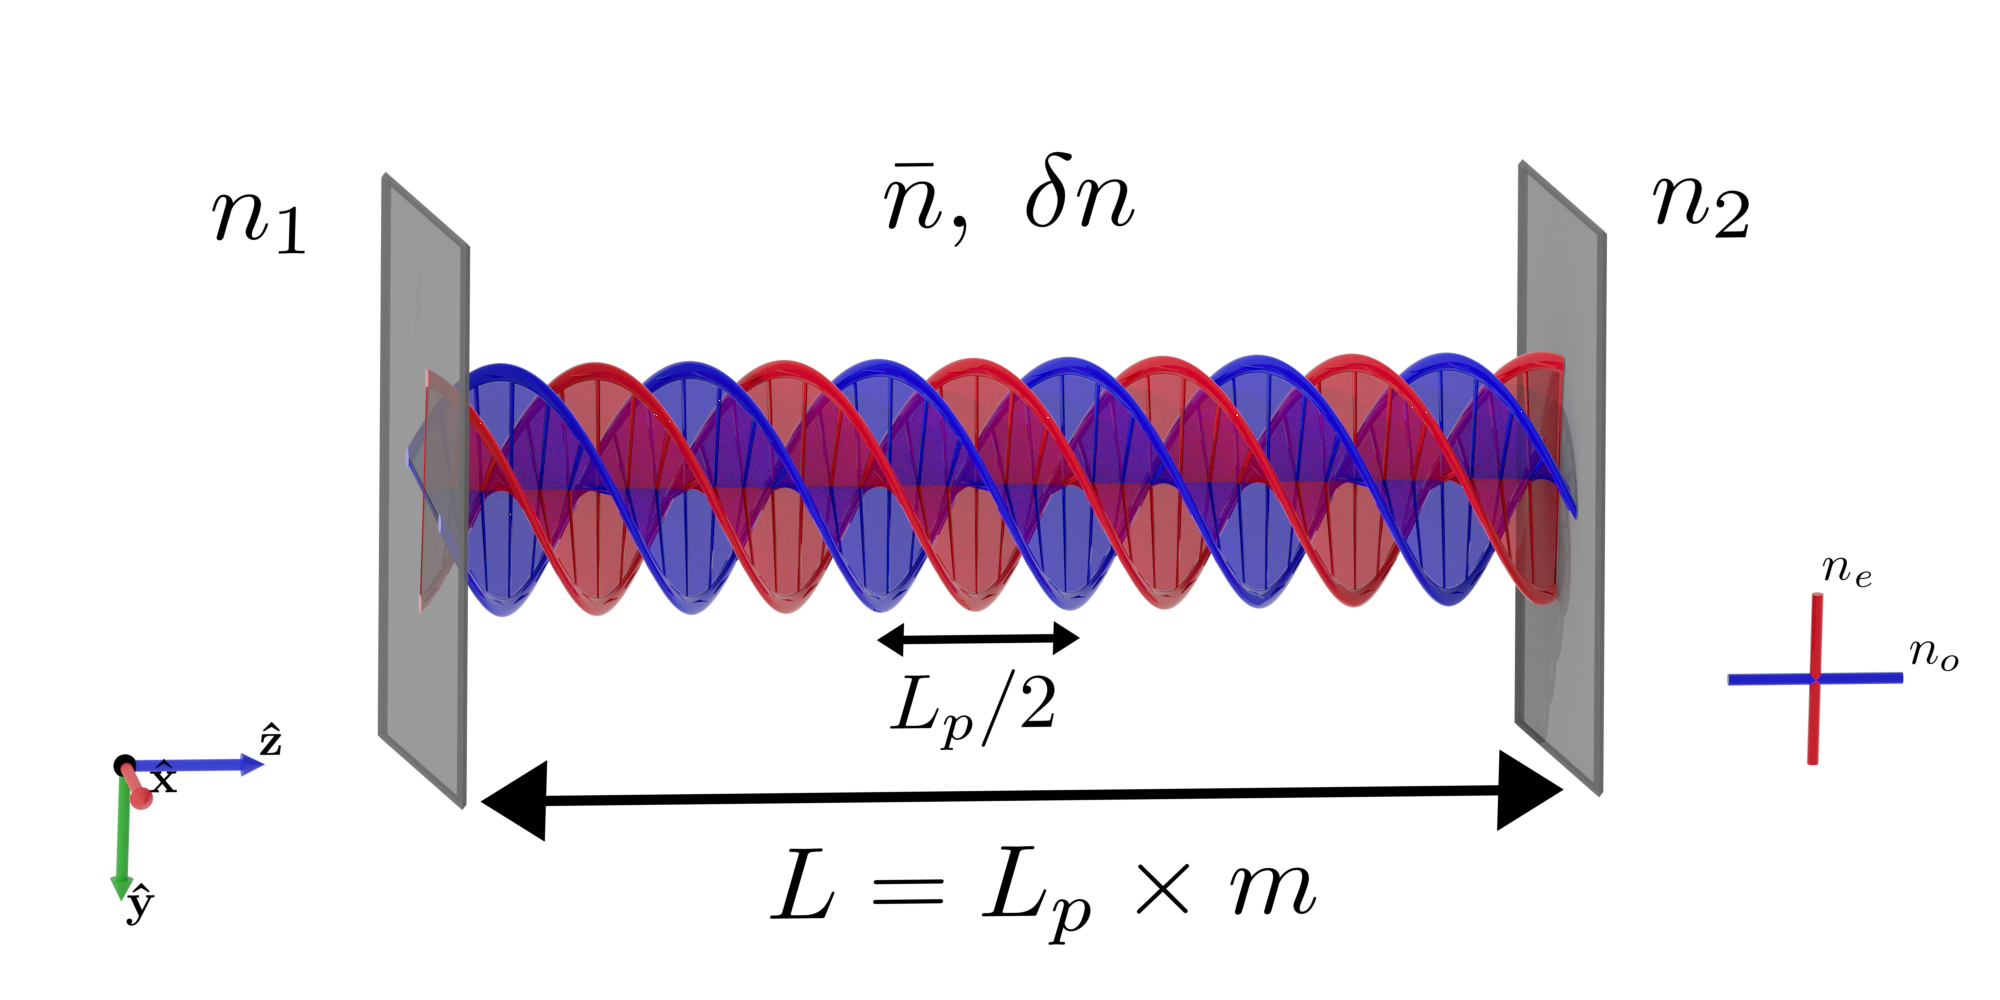
\includegraphics[width=\linewidth]{images/simple_cavity}
		\caption[Simple cavity]{Simple cavity}
		\label{fig:simple_cavity}
	\end{subfigure}
	\begin{subfigure}{0.58\linewidth}
		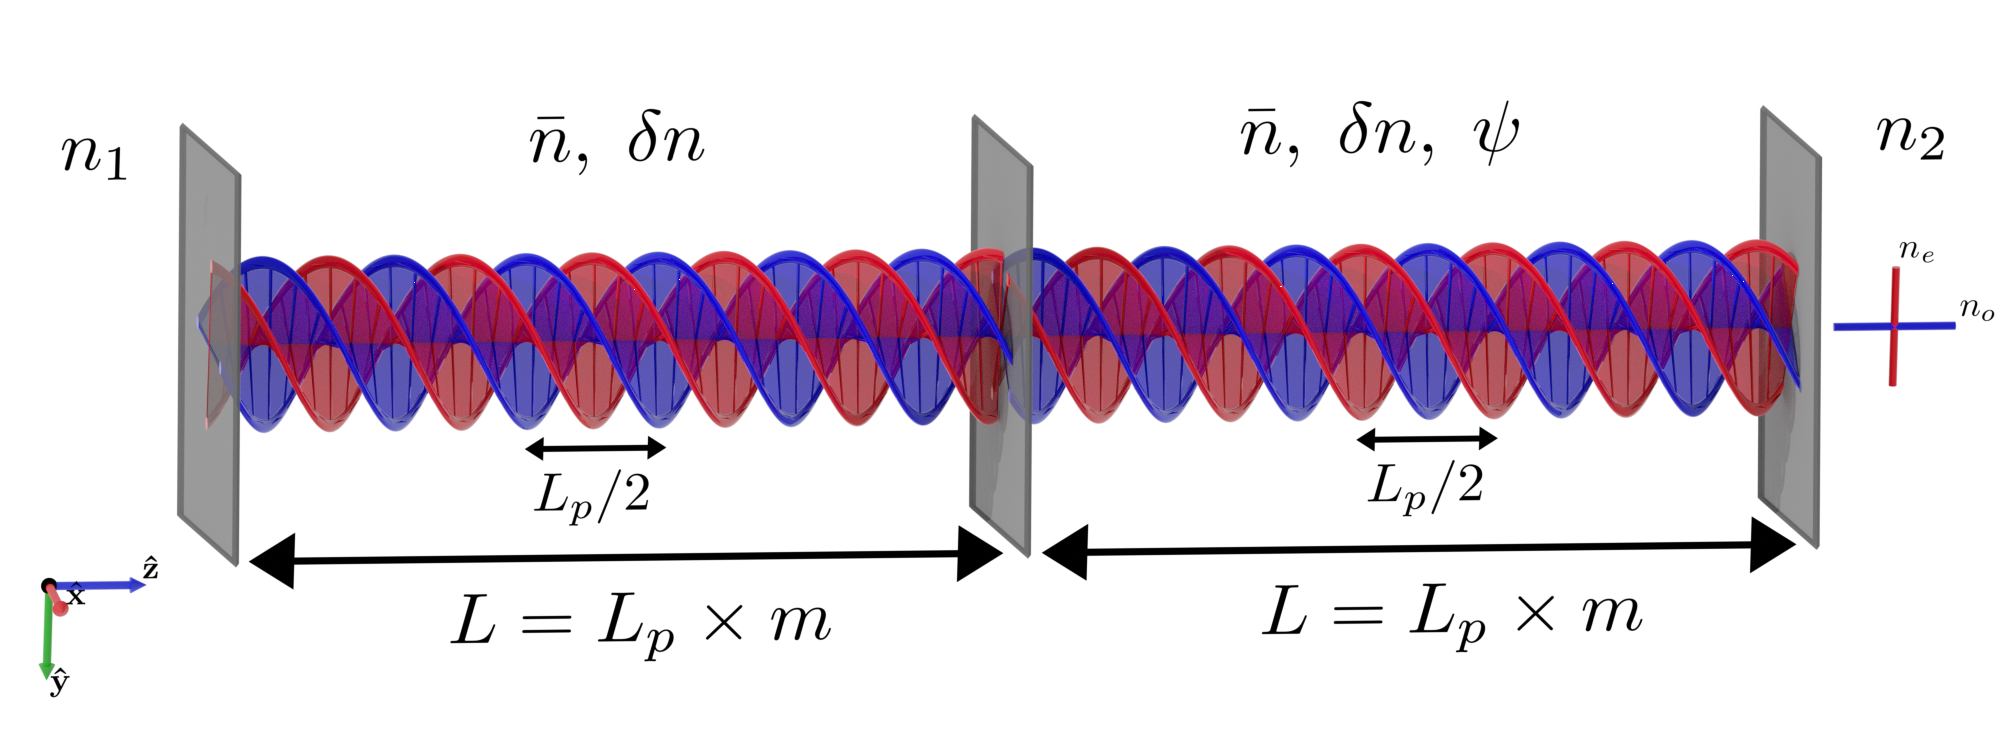
\includegraphics[width=\linewidth]{images/defect.png}
		\caption{Cavity with a defect}
		\label{fig:defect}
	\end{subfigure}
	\begin{subfigure}{\linewidth}
		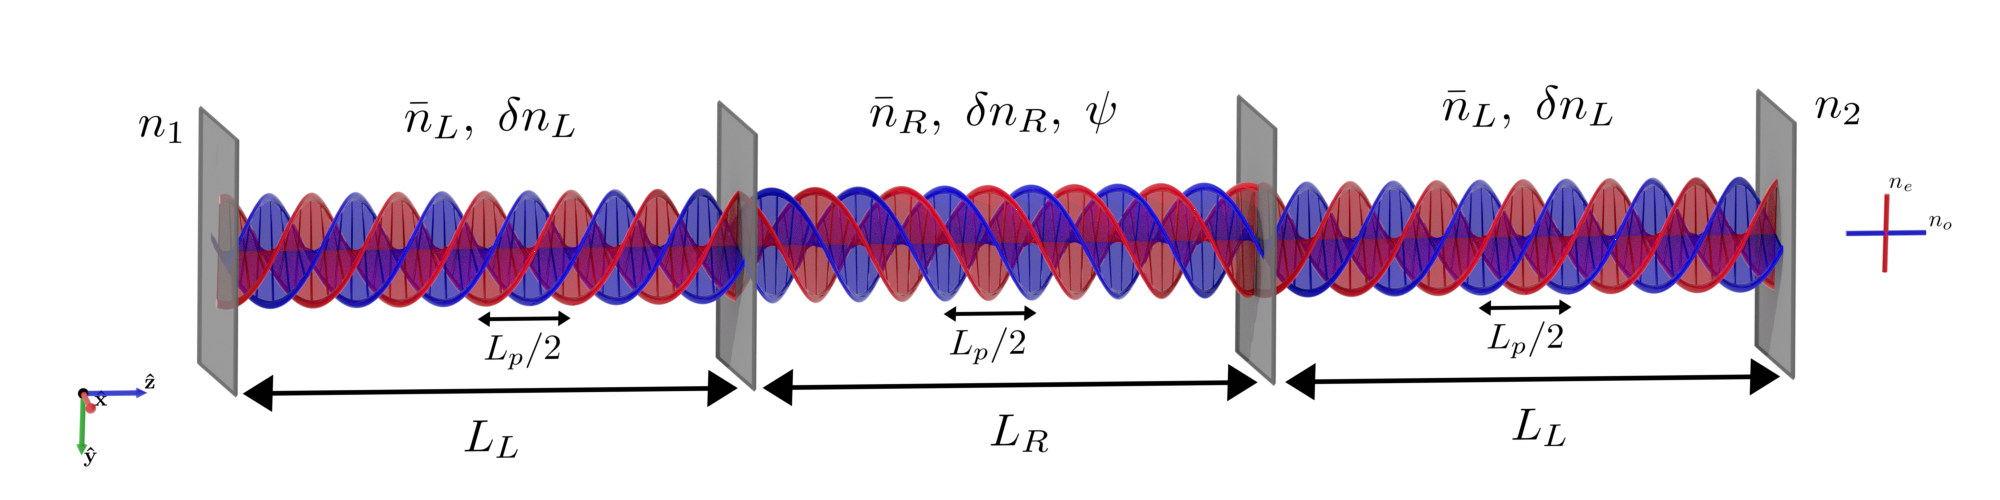
\includegraphics[width=\linewidth]{images/hybrid.png}
		\caption{Hybrid cavity}
		\label{fig:hybrid}
	\end{subfigure}
	\begin{subfigure}{\linewidth}
		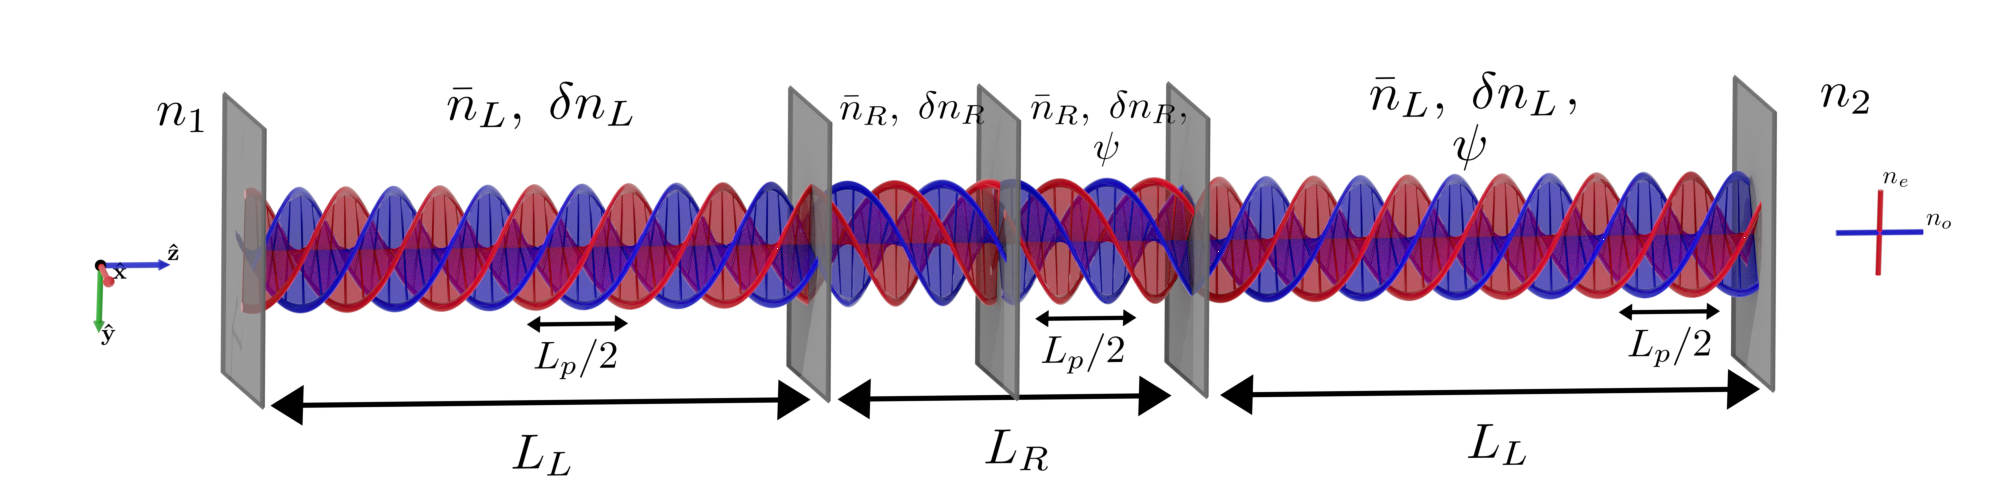
\includegraphics[width=\linewidth]{images/hybrid_defect.png}
		\caption{Hybrid defect cavity}
		\label{fig:hybrid_defect}
	\end{subfigure}
	\caption[Cavities modelled in this study]{Cavities modelled in this study.  For every cavity, $\bar{n}$ denotes an average refractive index, $\delta n$ a birefringence and $p=\frac{2\pi}{L_p}$ a periodicity. They are surrounded by isotropic media of refractive indices $n_1$ and $n_2$. The cavity lengths are an integer multiple of $L_p$.}
	\label{fig:cavities_blender}
\end{figure}
\chapter{Method}
Four cavities were modelled, using coupled wave theory and exact theory, during this project. Firstly a simple cavity reproducing the results proposed by Topf and McCall\cite{topf_modes_2014}, secondly a chiral cavity with a defect introduced at the centre of the cavity, then, a hybrid cavity composed of a right-handed medium placed between two left-handed media, and finally, a hybrid cavity similar to the previous one, except it has a defect in the centre. This chapter aims to describe the method used to ensure the correctness and a good understanding of the processes that are taking place inside the cavities.

\section{Reflectivity}

The first step to ensure the correctness of the simulation is to reproduce the reflectivity diagram presented in previous studies\cite{mccall_simplified_2009}. As the source code used to calculate those reflectivity diagrams is available, a direct comparison with the coupled wave and exact theories implementations used for this report is possible. The reflectivity of the cavity with a defect is also plotted for both simulation methods, as it is expected to give a very narrow filter because of the similarity with a quarter wavelength defect in a standard distributed Bragg reflector\cite{mccall_photonics_2020}. The reflectivity diagram for the third cavity was not examined.

\section{Energy conservation}

To check the correctness of the models used, it is worth checking the energy conservation throughout a lossless medium. To compare coupled wave theory to exact theory, equations \ref{eq:energyconservationa}, \ref{eq:energyconservationb} and \ref{eq:energyconservationredistribution} are plotted for the each cavity, with the gain turned to zero.

\section{Conditions for lasing}
This section discusses the method used to detect cavity susceptible to allow lasing. Two equivalent conditions are presented, as well as the parameters examined.

\subsection{First lasing condition}
In order to characterize the round-trip of a ray in the cavity, we consider the field at $z=0^-$. The chiral medium is characterized by the matrix $\bm{M_c}$. Applying equation \ref{eq:pinv} yields equation \ref{eq:method:internal_pinv}.

\begin{equation}
\begin{bmatrix}
E_{L}^+(z=L^-) \\
E_{R}^+(z=L^-) \\
E_{L}^-(z=0^+) \\
E_{R}^-(z=0^+) \\
\end{bmatrix} = \left(\text{inv}_1(\bm{M_c})\right)^{-1}\begin{bmatrix}
E_{L}^+(z=0^+) \\
E_{R}^+(z=0^+) \\
E_{L}^-(z=L^-) \\
E_{R}^-(z=L^-) \\
\end{bmatrix}\label{eq:method:internal_pinv}
\end{equation}
Then, using equation \ref{eq:reflection}, it is possible to express the boundary condition at the interfaces with the isotropic media. Naming $\bm{R_1}$ and $\bm{R_2}$ the reflection matrices at interfaces 1 and 2, this yields equation \ref{eq:method:round_trip}, where $F_0$ and $F_1$ are the field vectors before and after a round trip.
\begin{equation}
F_1 = \begin{pmatrix}
\bm{0} & \bm{R_1}\\
\bm{R_2} & \bm{0}
\end{pmatrix}\left(\text{inv}_1(\bm{M_c})\right)^{-1}F_0 \label{eq:method:round_trip}
\end{equation}
Then it is straightforward to express the lasing condition as in equation \ref{eq:method:round_trip_det}, where $\bm{I}$ is the identity matrix.
\begin{equation}
\left|\begin{pmatrix}
\bm{0} & \bm{R_1}\\
\bm{R_2} & \bm{0}
\end{pmatrix}\left(\text{inv}_1(\bm{M_c})\right)^{-1} - \bm{I}\right| = 0 \label{eq:method:round_trip_det}
\end{equation}

\subsection{Second lasing condition}
\label{sec:lasing_condition}
This second method is simpler than the first and will be used to analyze the cavities. Its key advantage is that it allows using the propagation matrix describing the cavity as a "black box", that is, it is not necessary to be able to express the reflections at the interfaces. This allows simulating the cavities using the Oseen transformation.

Considering a cavity described by the propagation matrix $\bm{M_c}$, we have equation \ref{eq:method:propag}.

\begin{equation}
\begin{bmatrix}
E_{L}^+(z=L^+) \\
E_{R}^+(z=L^+) \\
E_{L}^-(z=L^+) \\
E_{R}^-(z=L^+) \\
\end{bmatrix} = \bm{M_c}\begin{bmatrix}
E_{L}^+(z=0^-) \\
E_{R}^+(z=0^-) \\
E_{L}^-(z=0^-) \\
E_{R}^-(z=0^-) \\
\end{bmatrix}\label{eq:method:propag}
\end{equation}
%
For a laser cavity, the boundary conditions are $E_{L}^-(z=L^+)=0,\;E_{R}^-(z=L^+)=0$ and $E_{L}^+(z=0^-)=0,\;E_{R}^+(z=0^-)=0$. Thus, writing $\bm{M_c}$ by $2\times2$ blocks, equation \ref{eq:method:propag} becomes
\begin{equation}
\begin{bmatrix}
E_{L}^+(z=L^+) \\
E_{R}^+(z=L^+) \\
0 \\
0 \\
\end{bmatrix} = \begin{pmatrix}
	\bm{M_{11}} & \bm{M_{12}}\\
	\bm{M_{21}} & \bm{M_{22}}
\end{pmatrix}\begin{bmatrix}
0 \\
0 \\
E_{L}^-(z=0^-) \\
E_{R}^-(z=0^-) \\
\end{bmatrix}
\end{equation}
%
Then a simple condition for lasing can be expressed by equation \ref{eq:method:lasing_condition}.
\begin{equation}
\left|\bm{M_{22}}\right| = 0 \label{eq:method:lasing_condition}
\end{equation}

\subsection{Parameters of the simulations}

The parameters explored in this study are gain and detuning of the medium. Those two quantities are defined from $\delta k$, introduced in section \ref{sec:cwt}, and $L$ the length of the medium considered. Denoting gain and detuning respectively $g$ and $d$,
\begin{eqnarray}
	g &=& - \Im{\frac{\delta k}{2}L}\\
	d &=& \Re{\frac{\delta k}{2}L}
\end{eqnarray}
%
The coupling $\kappa$ for all the chiral media is fixed to $\kappa=4/L$, and the periodicity of the medium, $L_p$, is fixed to 300nm.

These parameters cannot be used directly with Oseen transformation. However $k$, the wave-vector in the medium, and thus $\bar{n}$ can be determined directly from $\delta k$, allowing to calculate the permittivities $\epsilon_{a,b}$ as follow.
\begin{eqnarray}
\epsilon_a &=& \bar{n}^2 + \frac{2\kappa\bar{n}}{k_0}\\
\epsilon_b &=& \bar{n}^2 - \frac{2\kappa\bar{n}}{k_0}
\end{eqnarray} 

To provide better visualisation of lasing modes, as well as enable their automatic detection, the modelisations described in this report use the logarithm of the invert of equation \ref{eq:method:lasing_condition}. Thus, favourable lasing conditions can be identified as sharp peaks on the plots.



\section{Output polarization and intensity distribution of the modes}
\label{sec:output_pol}
It is then possible characterize the modes outputted by the cavity. Indeed, once the lasing cavities have been identified using method described in section \ref{sec:lasing_condition}, the corresponding output mode is found by taking the eigenvector of $\bm{M_{22}}$ with a 0 eigenvalue\footnote{In the simulations, the eigenvector with the smallest absolute eigenvalue is chosen.}.
\subsection{Comparison of the output polarisation ellipse}

The field is expressed in the cartesian or electromagnetic basis\footnote{In the case of a laser cavity, since there is not field coming towards the cavity, $E_{x,y}^-(z<0)=E_{x,y}(z<0)$}. Then, defining $R$ and $\delta$ as in equation \ref{eq:method:Rdelta},
\begin{equation}
R = \atan(|E_x|+|E_y|),\;\delta = \arg(E_y) - \arg(E_x) \label{eq:method:Rdelta}
\end{equation}
it is possible to calculate angle $\epsilon$ and orientation $\theta$ of the ellipse as in equations \ref{eq:method:epsilon} and \ref{eq:method:theta}\cite{weir_optical_2019}.
\begin{eqnarray}
\epsilon &=& \frac{1}{2}\asin(\sin(2R)|\sin(\delta)|) \label{eq:method:epsilon}\\
\theta &=& \frac{1}{2}\atan(\tan(2R)\cos(\delta)) \label{eq:method:theta}
\end{eqnarray}
$\epsilon$ and $\theta$ relate to the output polarization ellipse as in figure \ref{fig:ellipse}. The handedness of the ellipse can be determined from the sign of $\delta$, but since all calculations in this study are carried in the circular basis, it is simpler to look at the amplitude of $E_L$ and $E_R$. The polarizations outputted by the cavities is compared \textit{via} their corresponding values of $\epsilon$ and $\theta$, as well as the handedness of the ellipse.

In order to draw the ellipse, the cartesian form is used, and then rotated by angle $\theta$. The semi-major and semi-minor axes, $a$ and $b$, relate to $\epsilon$ as in equation \ref{eq:tanepsilon}. Thus, $\epsilon$ gives a good measure of how close to a circular polarisation the output is, as a circle would present $\epsilon=45^\circ$.
\begin{equation}
\frac{b}{a}=\tan(\epsilon) \label{eq:tanepsilon}
\end{equation}
%
Then, the points of the ellipse, before rotation, verify equation \ref{eq:epsilon}.
\begin{equation}
R^2 = ax^2+by^2\label{eq:ellipse}
\end{equation}


\begin{figure}
	\centering
	\begin{tikzpicture}[scale=2]
		\fill[color=gray!40] (0.5,0) arc (0:30:0.5) -- (0,0) -- (0.5,0);
		\draw (0.5,0.15) node[right] {$\theta$};
		\begin{scope}[rotate=30]
			\fill[color=gray!40] (1.5,0) arc (-180:-194:0.5) -- (2,0) -- cycle;
			\draw[color=gray!90] (0,0) ellipse (2 and 0.5);
			\draw[dotted] (-2.2,0) -- (2.2,0);
			\draw[dotted] (0,-0.7) -- (0,0.7);
			\draw[dotted] (2,0) -- (0,0.5);
			\draw (1.3,0.25) node[below right] {$\epsilon$};
			\draw[decoration={brace,mirror,raise=1.5pt},decorate]
			(0,0.5) -- node[left=1pt] {$b$} (0,0);
			\draw[decoration={brace,mirror,raise=1.5pt},decorate]
			(-2,0) -- node[below right=1pt] {$a$} (0,0);
		\end{scope}
		\draw [thick, ->] (0,-1.3) -- (0,1.3);
		\draw (2,0) node[right] {$x$};
		\draw [thick, ->] (-2,0) -- (2,0);
		\draw (0,1.3) node[above] {$y$};
	\end{tikzpicture}
	\caption[Parameters of an ellipse]{Parameters of the ellipse. $\theta$ is the rotation of the axes, $a$ is the semi-major axis, $b$ the semi-minor axis and $\epsilon$ relates to $a$ and $b$ as $\frac{b}{a}=\tan(\epsilon)$.}
	\label{fig:ellipse}
\end{figure}

\subsection{Intensity distribution}
\label{sec:intensity_distribution}

Knowing the eigen vector of $\bm{M_{22}}$ allows to fully retrieve the field for $z=0^-$, as it is assumed no light goes towards the cavity, \textit{i.e.} $E_{L,R}^+(z=0^-) = 0$. It is then possible to calculate the field at each point $z'$ of the cavity by simply calculating the corresponding matrix. For example if a cavity is described by 
\begin{equation}
\bm{M} = \prod_{j}\bm{M_j}
\end{equation}
where $\bm{M_j}$ describes the slab of medium between $z_j$ and $z_{j+1}$, and $z_k < z' \leq z_{k+1}$, then the field at $z'$ is given by equation \ref{eq:method:Fzprime}.
\begin{equation}
F(z') = \bm{M_{z'}}\prod_{j=0}^{k-1}\bm{M_j} \cdot F_0 \label{eq:method:Fzprime}
\end{equation}
Where $F_0$ is the field at $z=0^-$ and $\bm{M_{z'}}$ describes a slab of medium with the same characteristics as $\bm{M_{k}}$, except it has a length of $z'-z_k$.

It is finally possible to calculate the total intensity at $z'$.
\begin{equation}
I = \norm{\bm{E}}^2
\end{equation}

In case $F$ is expressed in the circular basis, it can be useful to plot the intensities corresponding to each component of the field. Thus, we define $I_{L,R}^{\pm} = \abs{E_{L,R}^\pm}^2$. 
\chapter{Results}
This part presents the results obtained for the four cavities modelled. First, the simple cavity is used to gauge the quality of the implementation, both regarding previous studies and the comparison between approximate and exact theory. Then the results for the three new cavity designs are given in term of reflectivity when this is relevant and of output polarisation and intensity distribution. This allows to determinate the dynamics that lead the cavity to lase.
\section{Simple cavity}
\label{sec:simple_cavity}

We consider a slab of chiral medium characterized by periodicity $p$, average refractive index $\bar{n}$ and birefringence $\delta n$ between two isotropic media of refractive indices $n_1$ and $n_2$. Figure \ref{fig:simple_cavity} schematizes the cavity.

\subsection{Reflectivities}

To ensure the correctness of the implementation of coupled wave theory and exact theory, the reflection coefficients yielded by both methods are plotted in figure \ref{fig:simple_cavity:reflection}. The parameters used for this simulation are given in table \ref{tab:simple_cavity:reflection}. The original study took into account the angle of the plane wave in respect of $z$. Although it would be possible to do so here as well, the choice was made to only consider plane waves propagating along $\bm{z}$ axis. To fit the parameters of the previous study, $\epsilon_a$ was thus tuned to take into account the relative permittivity a plane wave propagating along another axis than $\bm{z}$.

The results given by both theories are satisfactory and approximate theory matches fairly well exact theory, with variations up to $1\%$ on the band edges. However, it can be noted that the results given in \cite{mccall_simplified_2009} are closer to exact theory than what appears in figure \ref{fig:simple_cavity:reflection}. This is because the reflection coefficients derived there use Fresnel formulas rather than the method described in section \ref{sec:interface_iso}. It appears that Fresnel coefficients are more exact. This hints that it may be possible to derive more precise matrices to switch between circular and electromagnetic bases.

\begin{table}
	\centering
	\begin{tabulary}{\linewidth}{LCC}
		\hline
		\hline
		Structural period of the chiral medium & $L_p$ & 300 nm \\
		Length of the chiral medium & $L$ & $20\times L_p$ \\
		Refractive index of the surrounding media & $n_1$ & 1 \\
		 & $n_2$ & 2 \\
		Relative permittivity $a$ & $\epsilon_a$ & $3.0897 + 0.0201i$ \\
		Relative permittivity $b$ & $\epsilon_b$ & $2.9+0.02i$ \\
		\hline
		\hline
	\end{tabulary}
	\caption[Parameters for the simple cavity]{Parameters used to calculate reflectivities. Those are equivalent to the parameters used in \cite{mccall_simplified_2009}.}
	\label{tab:simple_cavity:reflection}
\end{table}

\begin{figure}
	\centering
	\begin{subfigure}{0.32\linewidth}
		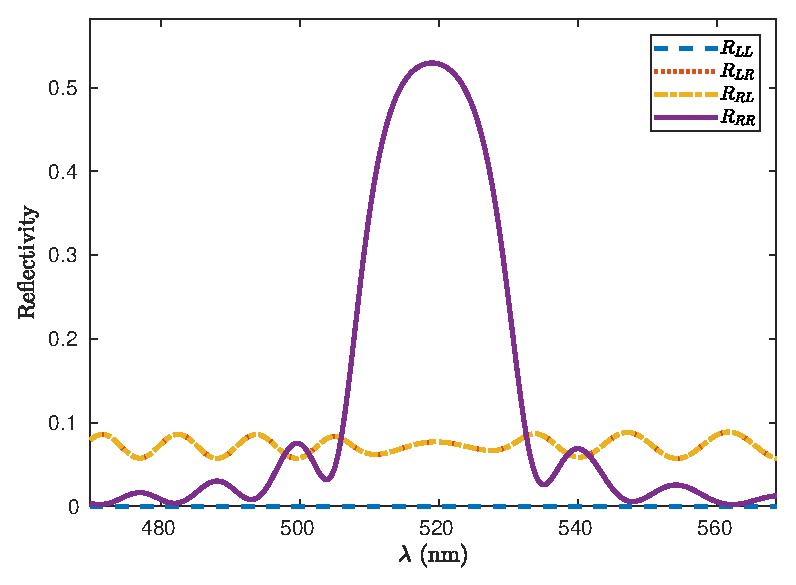
\includegraphics[width=\linewidth]{plots/simple/reflection_oseen}
		\caption{}
		\label{fig:simple_cavity:reflection_oseen}
	\end{subfigure}
	\begin{subfigure}{0.32\linewidth}
		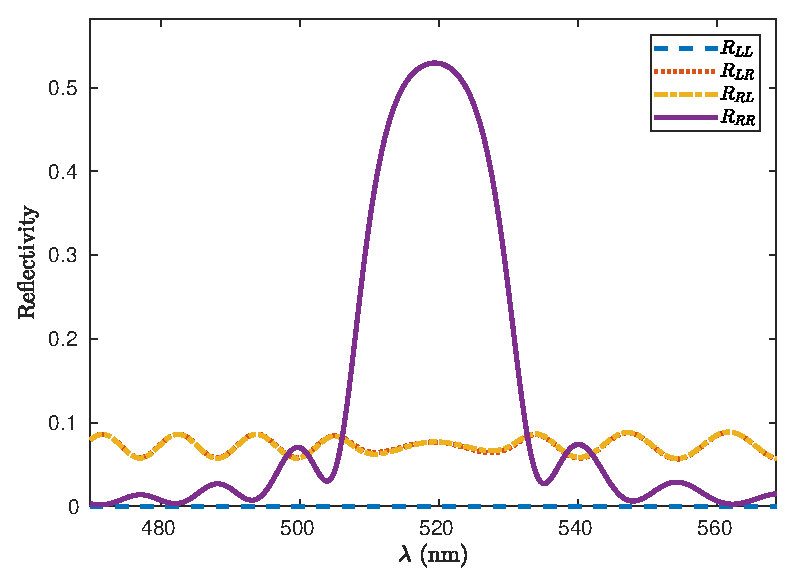
\includegraphics[width=\linewidth]{plots/simple/reflection_cwt}
		\caption{}
		\label{fig:simple_cavity:reflection_cwt}
	\end{subfigure}
	\begin{subfigure}{0.32\linewidth}
		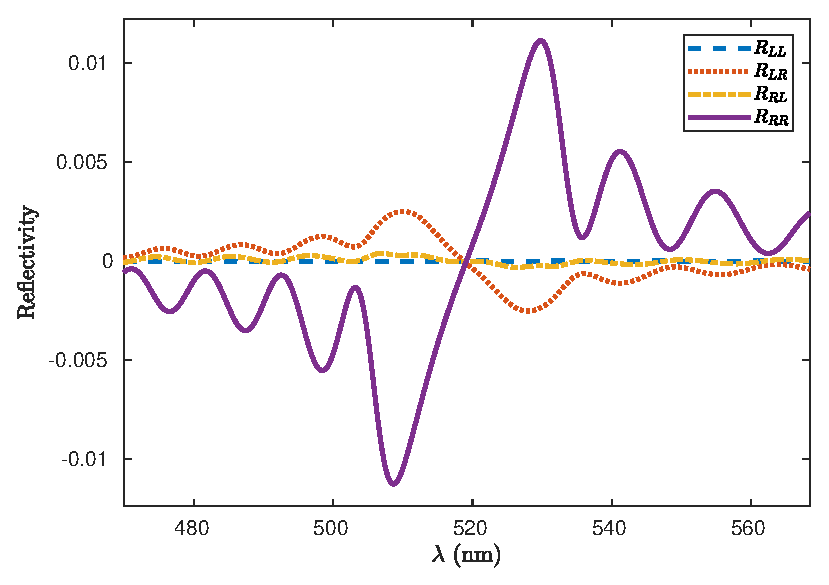
\includegraphics[width=\linewidth]{plots/simple/reflection_comp}
		\caption{}
		\label{fig:simple_cavity:reflection_comp}
	\end{subfigure}
	\begin{subfigure}{0.32\linewidth}
		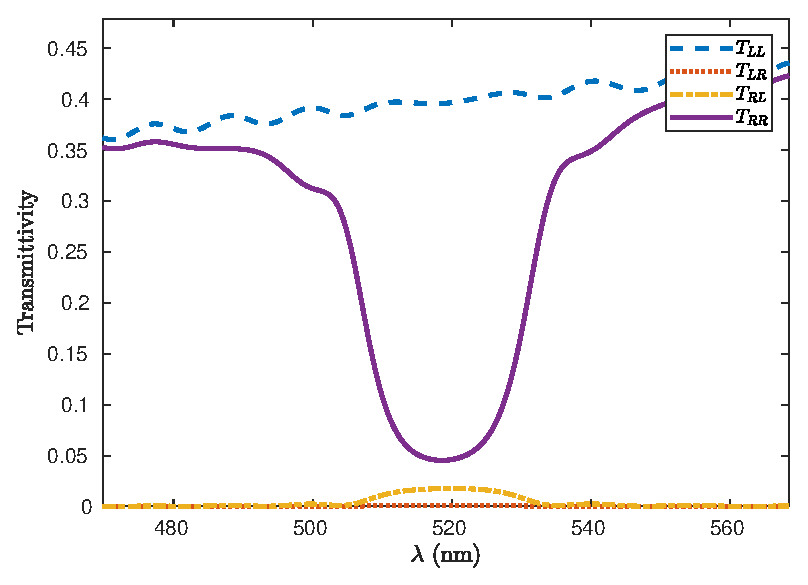
\includegraphics[width=\linewidth]{plots/simple/transmission_oseen}
		\caption{}
		\label{fig:simple_cavity:transmission_oseen}
	\end{subfigure}
	\begin{subfigure}{0.32\linewidth}
		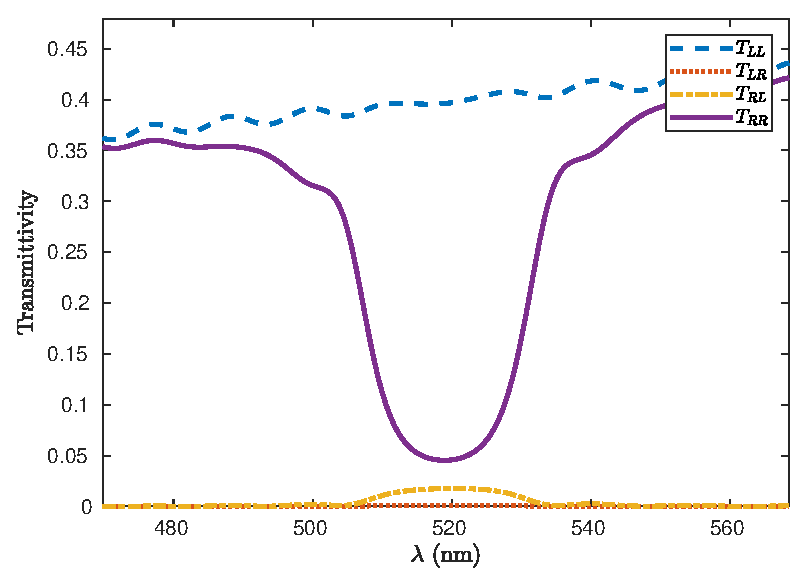
\includegraphics[width=\linewidth]{plots/simple/transmission_cwt}
		\caption{}
		\label{fig:simple_cavity:transmission_cwt}
	\end{subfigure}
	\begin{subfigure}{0.32\linewidth}
		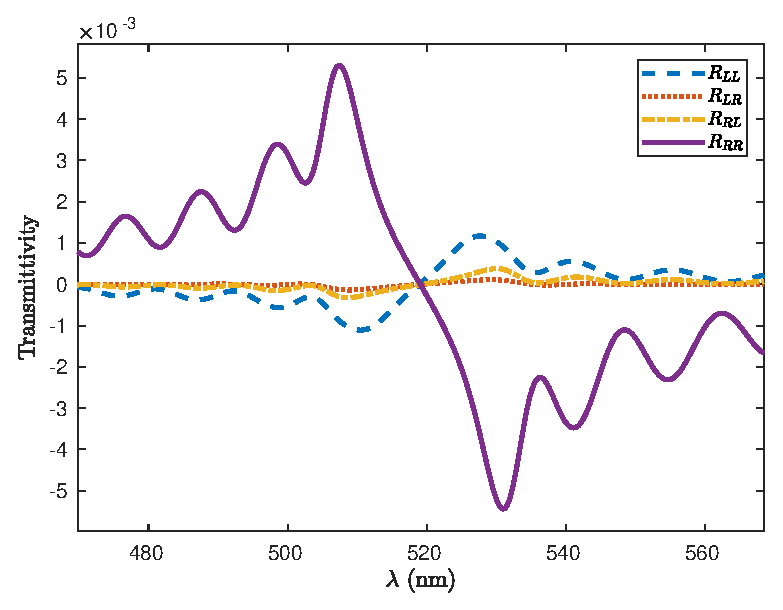
\includegraphics[width=\linewidth]{plots/simple/transmission_comp}
		\caption{}
		\label{fig:simple_cavity:transmission_comp}
	\end{subfigure}
	\caption[Comparison of reflectivities and transmittivities for a simple cavity]{Comparison of reflectivities and transmittivities for a simple cavity of right-handed medium. (\protect\tikz[baseline=-0.5ex]{\protect\draw[color=blue, dashed, thick] (0,0) -- (2ex,0) ;} $R_{LL}$, \protect\tikz[baseline=-0.5ex]{\protect\draw[color=red, dotted, thick] (0,0) -- (2ex,0) ;} $R_{LR}$, \protect\tikz[baseline=-0.5ex]{\protect\draw[color=orange, dashdotted, thick] (0,0) -- (2ex,0) ;} $R_{RL}$, \protect\tikz[baseline=-0.5ex]{\protect\draw[color=purple, solid, thick] (0,0) -- (2ex,0) ;} $R_{RR}$).
	\ref{fig:simple_cavity:reflection_oseen} Reflectivities calculated with the Oseen method. \ref{fig:simple_cavity:reflection_cwt} Reflectivities calculated with the coupled wave theory. \ref{fig:simple_cavity:reflection_comp} Comparison of reflectivities obtained with the two methods. \ref{fig:simple_cavity:transmission_oseen} Transmittivities calculated with the Oseen method. \ref{fig:simple_cavity:transmission_cwt} Transmittivities calculated with the coupled wave theory. \ref{fig:simple_cavity:transmission_comp} Comparison of transmittivities obtained with the two methods.}
	\label{fig:simple_cavity:reflection}
\end{figure}

\subsection{Energy conservation}

The second verification made was upon energy conservation. The only comparison possible here is between exact and approximate theory. Figure \ref{fig:simple_cavity:energy_conservation} shows the comparison of the three measures of energy conservation for both exact and approximate theories. As expected, exact theory conserves energy down to machine precision, while approximate theory ensure less precisely the conservation of energy, especially its redistribution between left and right-handed polarised light.

\begin{figure}
	\centering
	\begin{subfigure}{0.49\linewidth}
		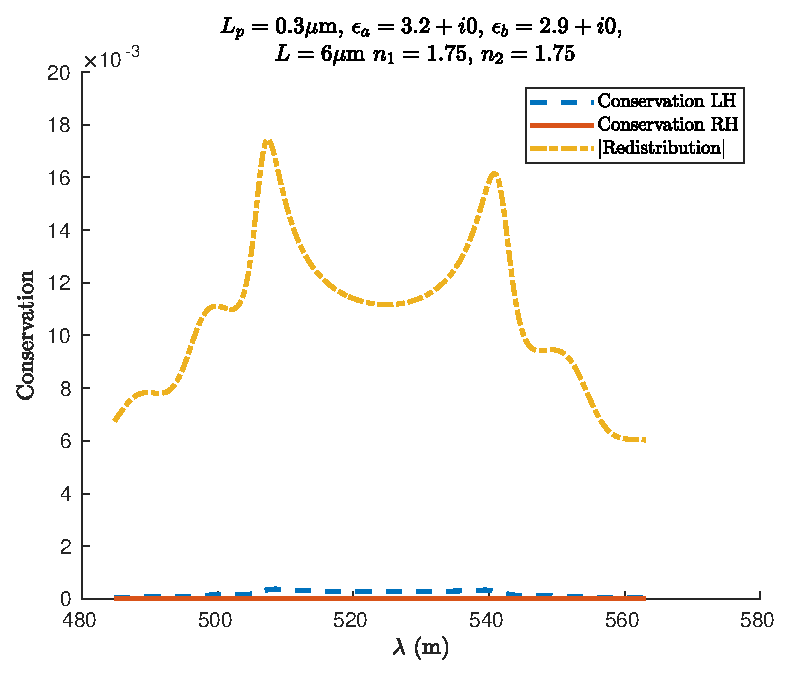
\includegraphics[width=\linewidth]{plots/simple/energy_cwt}
		\caption{}
		\label{fig:energy_cwt}
	\end{subfigure}
	\begin{subfigure}{0.49\linewidth}
		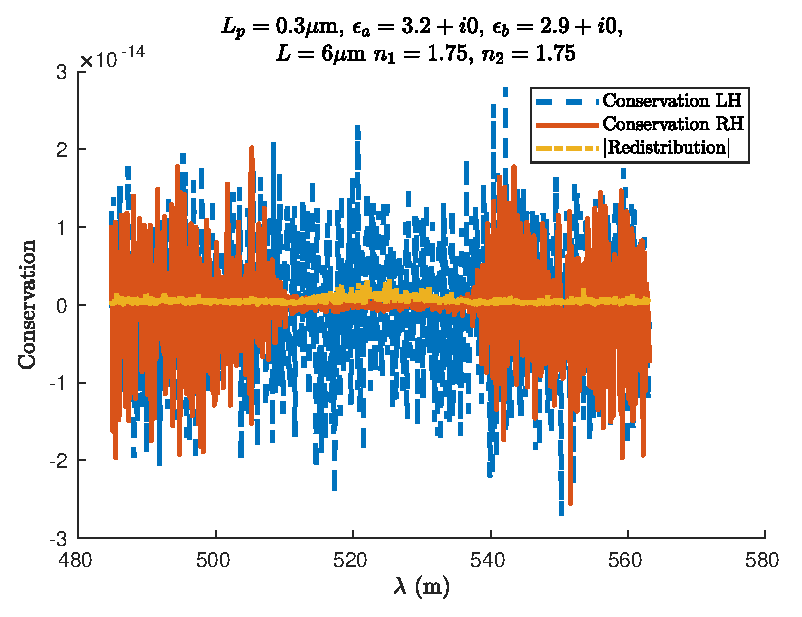
\includegraphics[width=\linewidth]{plots/simple/energy_oseen}
		\caption{}
		\label{fig:energy_oseen}
	\end{subfigure}
	\caption[Energy conservation in a simple cavity]{Energy conservation in a simple cavity. \ref{fig:energy_cwt} Coupled wave theory. \ref{fig:energy_oseen} Oseen method.}
	\label{fig:simple_cavity:energy_conservation}
\end{figure}

\subsection{Comparing laser action}

Equation \ref{eq:method:lasing_condition} is then compared to the result given by Topf and McCall\cite{topf_modes_2014}. The parameters used for the simulation are the same as in the original paper, and are reproduced in table \ref{tab:simple_cavity:simulation}. Figure \ref{fig:simple_cavity:surf} shows the invert of the determinant found using the approach described by Topf and McCall, developed CWT and exact theory. This shows that the implementation of coupled wave theory proposed here is coherent with previous results and exact theory.

\begin{table}
	\centering
	\begin{tabulary}{\linewidth}{LCC}
		\hline
		\hline
		Structural period of the chiral medium & $L_p$ & 300 nm \\
		Length of the chiral medium & $L$ & $20\times L_p$ \\
		Refractive index of the surrounding media & $n_1=n_2$ & 1 \\
		Average refractive index of the chiral medium (Re) & $\bar{n}$ & 1.7690 \\
		Detuning range & $\mathrm{Re}(\delta k L / 2)$ & $[0,12]$ \\
		Gain range & $-\mathrm{Im}(\delta k L / 2)$ & $[0,2.5]$ \\
		Coupling constant & $\kappa$ & $4/L$\\
		\hline
		\hline
	\end{tabulary}
	\caption[Parameters for the simple cavity]{Parameters used for simulation. Those are the same as in \cite{topf_modes_2014} to allow comparison of the found modes.}
	\label{tab:simple_cavity:simulation}
\end{table}

\begin{figure}
	\centering
	\begin{subfigure}{0.32\textwidth}
		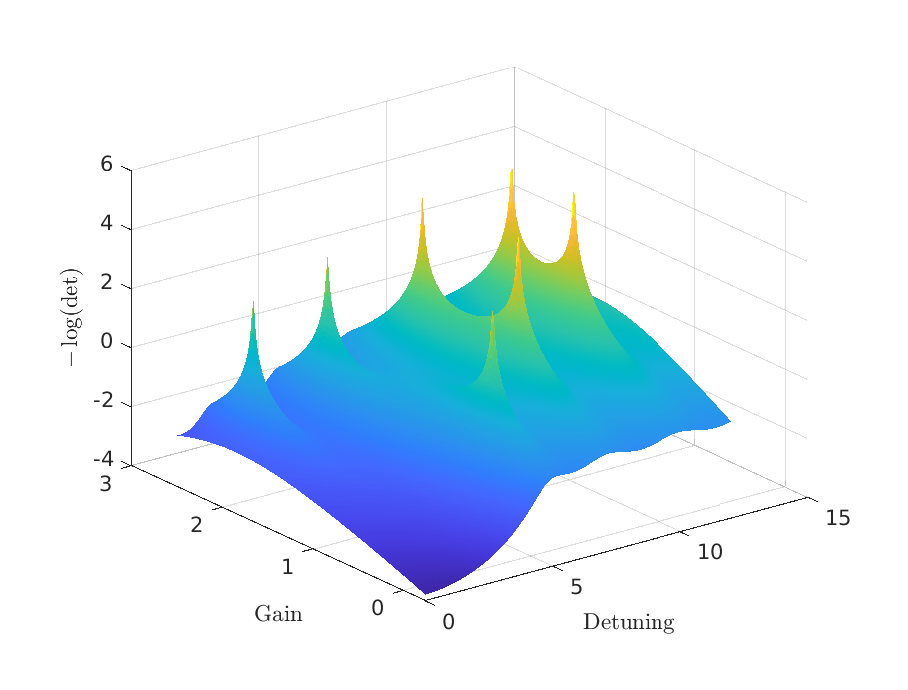
\includegraphics[width=\textwidth]{plots/simple/surface}
		\caption{}
		\label{fig:simple_cavity:mycwt_surf}
	\end{subfigure}
	\begin{subfigure}{0.32\textwidth}
		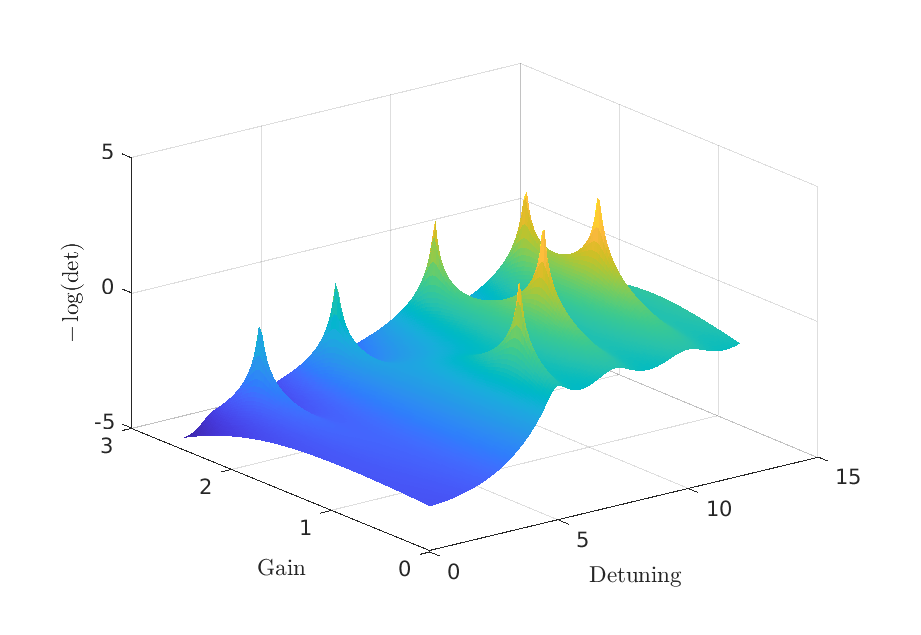
\includegraphics[width=\textwidth]{plots/simple/surface_topf}
		\caption{}
		\label{fig:simple_cavity:topf_surf}
	\end{subfigure}
	\begin{subfigure}{0.32\textwidth}
		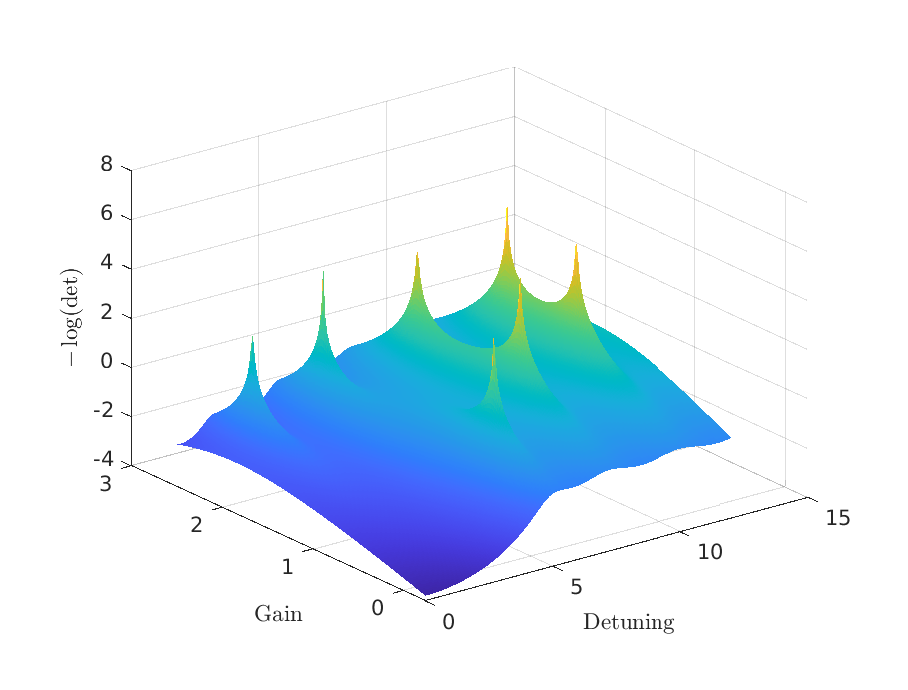
\includegraphics[width=\textwidth]{plots/simple/surface_oseen}
		\caption{}
		\label{fig:simple_cavity:oseen_surf}
	\end{subfigure}

	\begin{subfigure}{0.32\textwidth}
		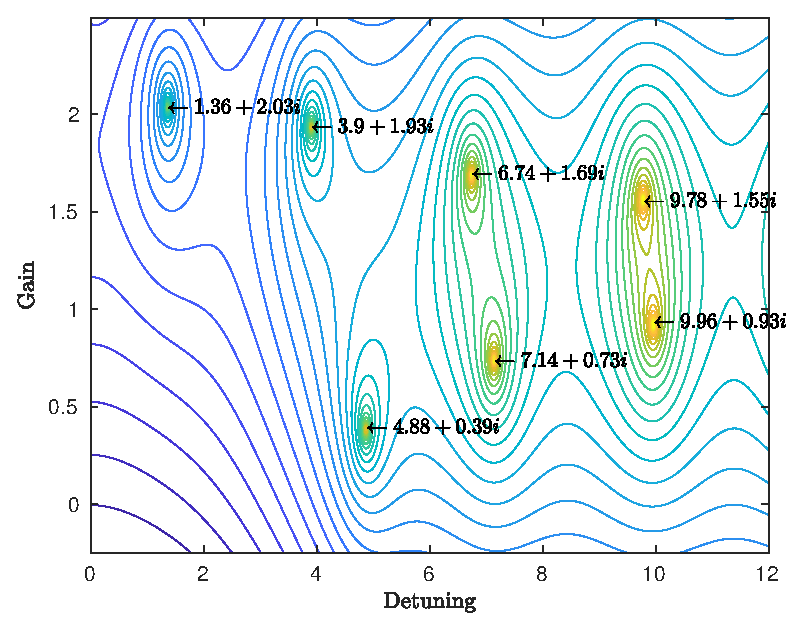
\includegraphics[width=\textwidth]{plots/simple/contour}
		\caption{}
		\label{fig:simple_cavity:mycwt_contour}
	\end{subfigure}
	\begin{subfigure}{0.32\textwidth}
		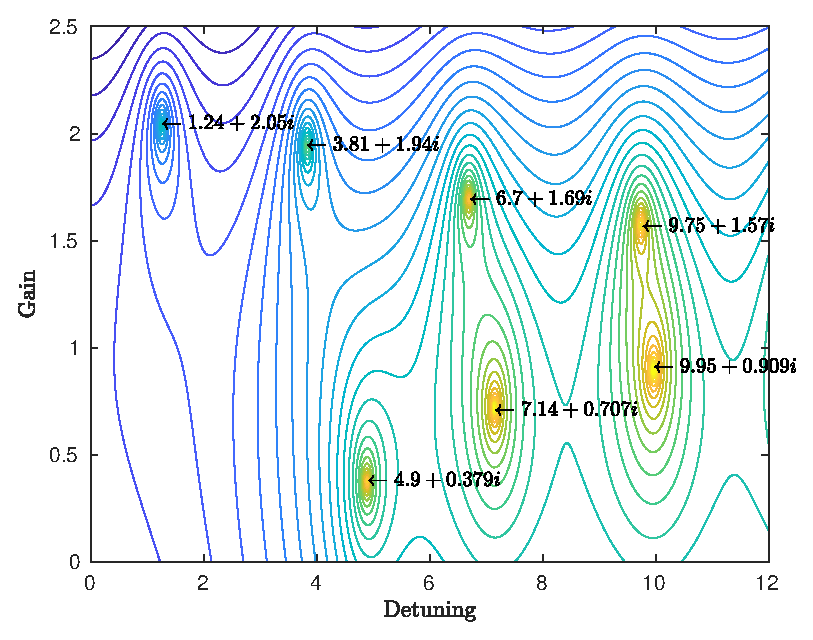
\includegraphics[width=\textwidth]{plots/simple/contour_topf}
		\caption{}
		\label{fig:simple_cavity:topf_contour}
	\end{subfigure}
	\begin{subfigure}{0.32\textwidth}
		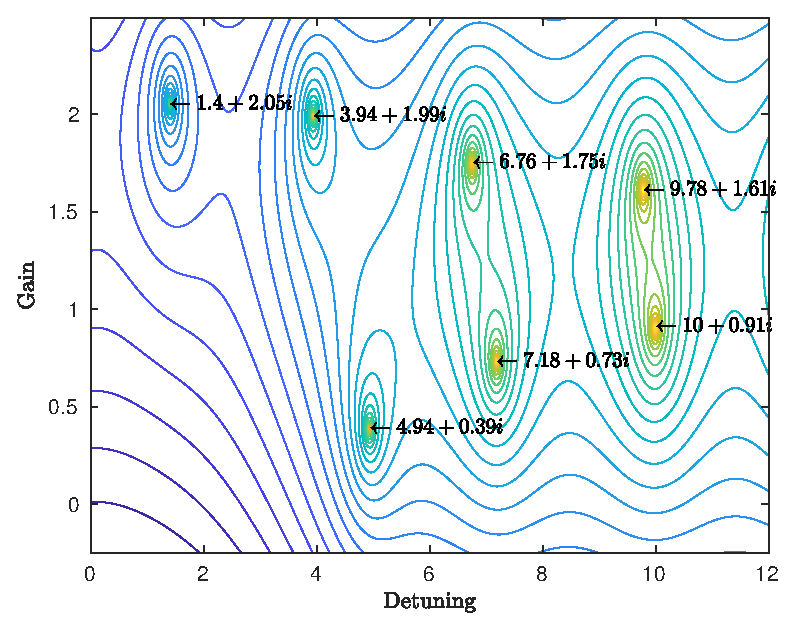
\includegraphics[width=\textwidth]{plots/simple/contour_oseen}
		\caption{}
		\label{fig:simple_cavity:oseen_contour}
	\end{subfigure}
	\caption[Comparison between methods for modeling a simple cavity.]{Comparison of the developed CWT and results reproduced from Topf and McCall\cite{topf_modes_2014}. \ref{fig:simple_cavity:mycwt_surf} shows the logarithm of the invert of the determinant of $\bm{M_{22}}$. \ref{fig:simple_cavity:mycwt_contour} is the corresponding contour plot where the lasing modes have been identified. \ref{fig:simple_cavity:topf_surf} is the invert of the determinant developed in \cite{topf_modes_2014} and \ref{fig:simple_cavity:topf_contour} is the corresponding contour plot. Finally \ref{fig:simple_cavity:oseen_surf} and \ref{fig:simple_cavity:oseen_contour} show the lasing coefficient obtained with the Oseen transformation.}
	\label{fig:simple_cavity:surf}
\end{figure}

Figure \ref{fig:simple_cavity:modes} shows the labelled output modes as well as the corresponding intensity distribution in the cavity. The first observation is that the overall intensity profile is, as expected, similar. The exact theory gives an account of the local variations in intensity due to the local variations of refractive index that are ignored in coupled wave theory. Moreover, coupled waves theory gives a good idea of the dynamics that take place in the cavity for each output mode. Indeed, for left-handed output polarisations, the intensity is mainly concentrated at the interfaces, corresponding to a Fabry-Pérot cavity where right-handed polarised light cannot propagate. On the other hand, for right-handed polarised light, Bragg reflections predominate.
\begin{figure}
	\centering
	\begin{subfigure}{.49\textwidth}
		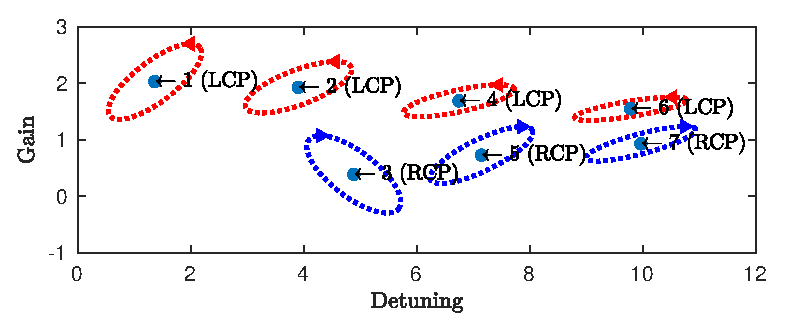
\includegraphics[width=\textwidth]{plots/simple/modes_found}
		\caption{Developed CWT}
		\label{fig:simple_cavity:modes_found}
	\end{subfigure}
	\begin{subfigure}{.49\textwidth}
		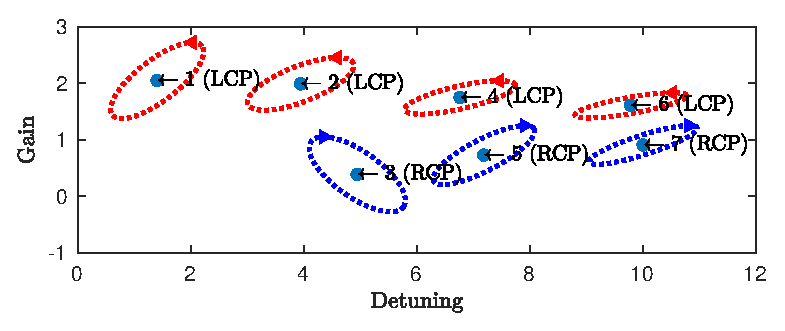
\includegraphics[width=\textwidth]{plots/simple/modes_found_oseen}
		\caption{Oseen method}
		\label{fig:simple_cavity:modes_found_oseen}
	\end{subfigure}
	\begin{subfigure}{.49\textwidth}
		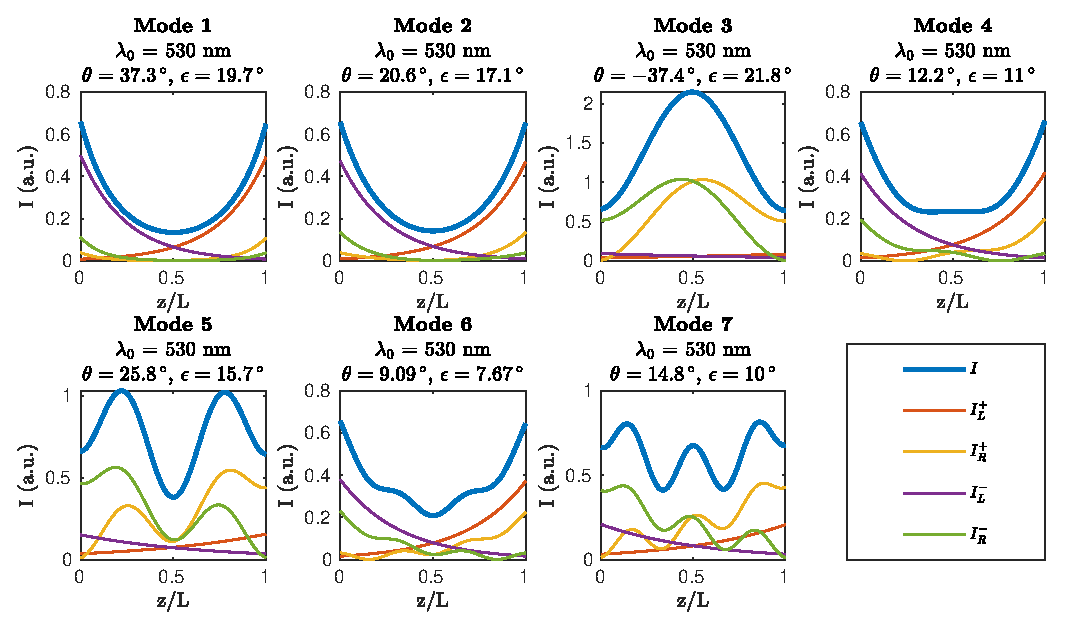
\includegraphics[width=\textwidth]{plots/simple/intensity_distribution}
		\caption{}
		\label{fig:simple_cavity:intensity_distribution}
	\end{subfigure}
	\begin{subfigure}{.49\textwidth}
		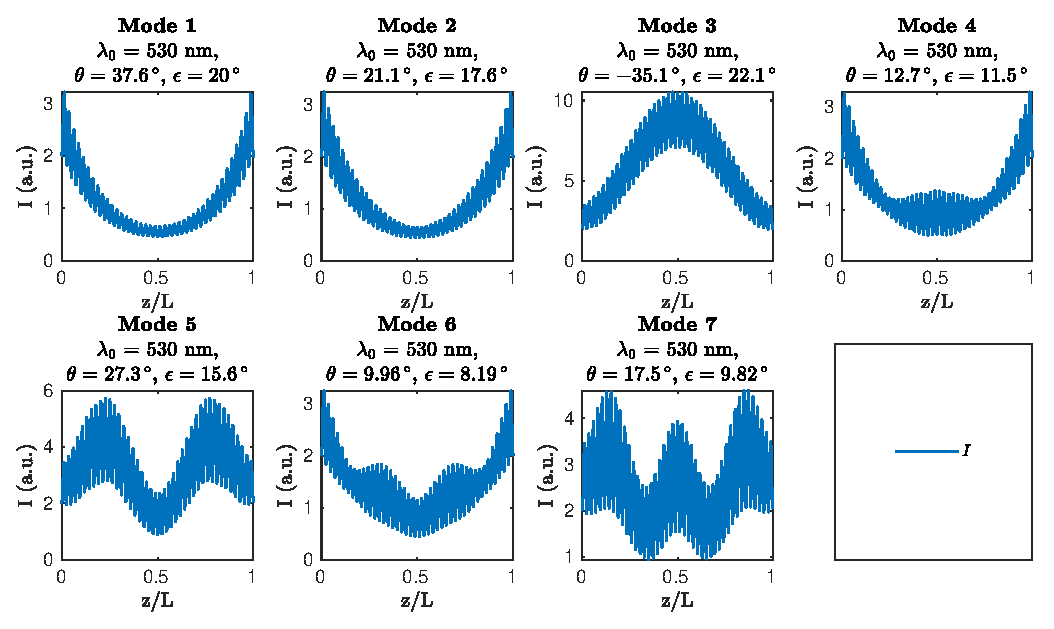
\includegraphics[width=\textwidth]{plots/simple/intensity_distribution_oseen}
		\caption{}
		\label{fig:simple_cavity:intensity_distribution_oseen}
	\end{subfigure}
	\caption[Comparison of intensity distribution for a simple cavity.]{\ref{fig:simple_cavity:modes_found} Labeled modes found with the developed CWT and corresponding output ellipses in medium 1. \ref{fig:simple_cavity:modes_found_oseen} Labeled modes found using exact theory and corresponding output ellipses. \ref{fig:simple_cavity:intensity_distribution} Intensity distribution in the cavity for the modes in \ref{fig:simple_cavity:modes_found}. \ref{fig:simple_cavity:intensity_distribution_oseen} Intensity distribution for modes given by exact theory.}
	\label{fig:simple_cavity:modes}
\end{figure}

\subsection{Conclusion on simple cavity}

This section mainly reproduced previous results, even though it introduced a comparison between coupled waves theory and exact theory that was not proposed before. Those results confirm that the implementation of both methods are fairly correct and increase the confidence in the new results proposed in the following sections, as they build on the same implementations.
\section{Cavity with a defect}
\label{sec:defect_cavity}
The first new geometry explored is a cavity with a defect. This is a cavity with geometry very similar to the one described in section \ref{sec:simple_cavity}, except that the helix is "broken" exactly at the centre of the cavity. This means the cavity is modelled by two identical chiral media, one of which as a start angle different from the other. This geometry is schematized in figure \ref{fig:defect}.

\subsection{Reflectivities}

As with the first cavity, the passive reflectivity is examined. This cavity is expected to behave as a very selective filter. Figure \ref{fig:defect_reflectivity} shows three reflectivity plots of right-handed cavities. The simplest is probably the first one, \ref{fig:defect_reflectivity:reflect}, with a $\frac{\pi}{2}$ defect and no losses. The narrow band filter behaviour is present at the Bragg wavelength, \textit{i.e.} $\Re{\bar{n}}\times L_p$\cite{mccall_simplified_2009}. Then, \ref{fig:defect_reflectivity:reflect_losses} shows that the introduction of losses in the medium decreases the filtering efficiency. Finally, by varying the angle of the defect, it is possible to tune the zero-reflectivity wavelength, as shown in figure \ref{fig:defect_reflectivity:reflect_other}. The transmitivities were also calculated, but do not show any remarkable feature that is not already displayed by reflectivities. Transmitivities are shown in appendix \ref{chap:transmitivities}.

\begin{figure}
	\centering
	\begin{subfigure}{0.49\linewidth}
		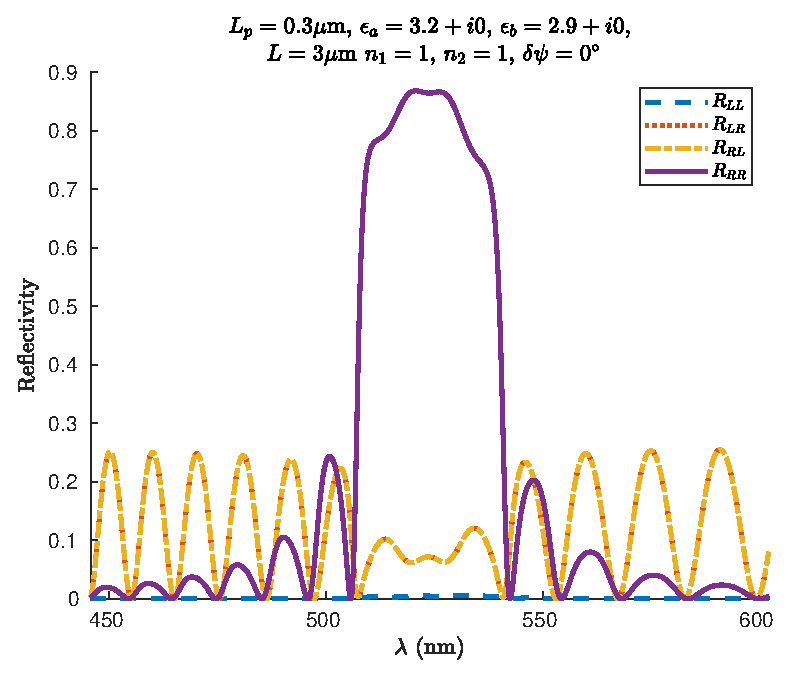
\includegraphics[width=\linewidth]{plots/defect/no_defect/oseen_reflection}
		\caption{}
		\label{fig:defect_reflectivity:reflect_nodefect}
	\end{subfigure}
	\begin{subfigure}{0.49\linewidth}
		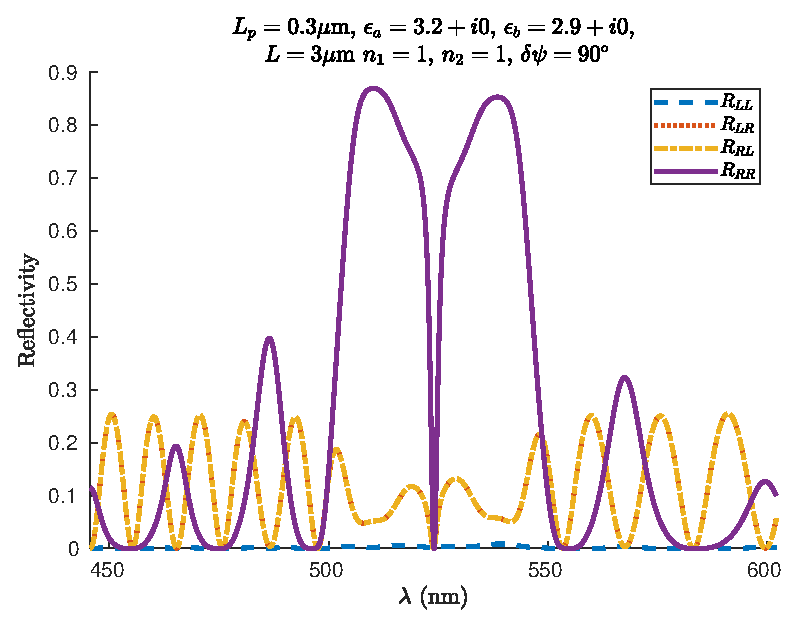
\includegraphics[width=\linewidth]{plots/defect/reflectivity/oseen_reflection}
		\caption{}
		\label{fig:defect_reflectivity:reflect}
	\end{subfigure}
	\begin{subfigure}{0.49\linewidth}
		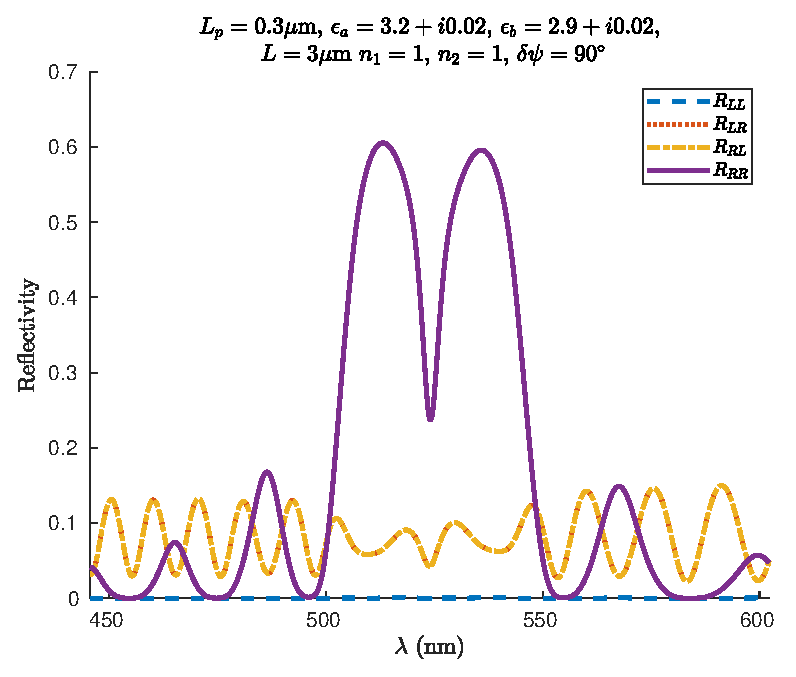
\includegraphics[width=\linewidth]{plots/defect/reflectivity_losses/oseen_reflection}
		\caption{}
		\label{fig:defect_reflectivity:reflect_losses}
	\end{subfigure}
	\begin{subfigure}{0.49\linewidth}
		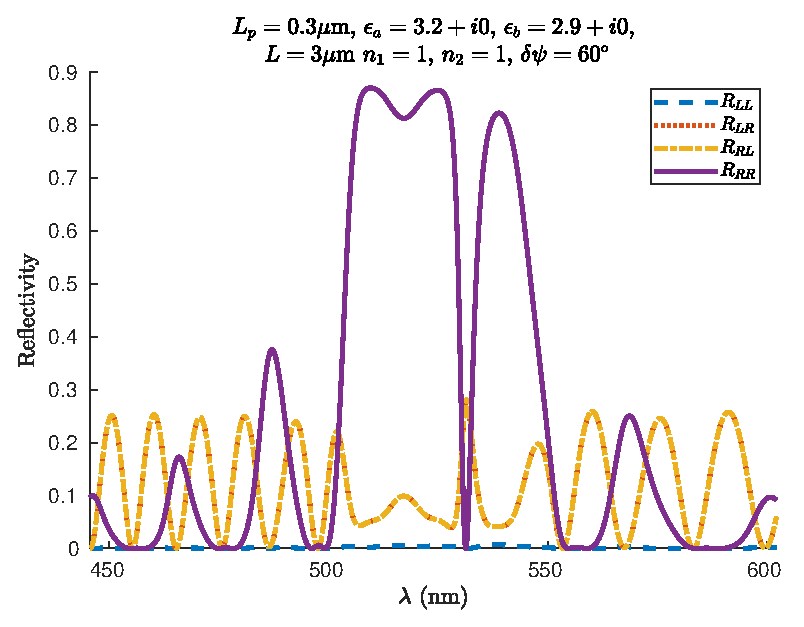
\includegraphics[width=\linewidth]{plots/defect/reflectivity_other_defect/oseen_reflection}
		\caption{}
		\label{fig:defect_reflectivity:reflect_other}
	\end{subfigure}
	\caption[Reflectivity of the narrow-band filter]{Reflectivities calculated for a right-handed cavity with a defect with the exact theory. Parameters are given on each figure. The results obtained with coupled wave theory are very close and a comparison is available in figures \ref{fig:reflectivities_narrow_appendix} and \ref{fig:reflectivities_narrow_appendix_comp} in appendix \ref{chap:reflectivities}. \ref{fig:defect_reflectivity:reflect_nodefect} Reflectivity without defect and without losses. \ref{fig:defect_reflectivity:reflect} Reflectivity for a defect of $\pi/2$ without losses. \ref{fig:defect_reflectivity:reflect_losses} Reflectivity for a defect of $\pi/2$ with losses. \ref{fig:defect_reflectivity:reflect_other} Reflectivity for a defect of $\pi/3$ without losses.}
	\label{fig:defect_reflectivity}
\end{figure}

\subsection{Laser action}

With the same methodology as before, lasing action is examined in the defect cavity. Figure \ref{fig:defect_cavity:surf} shows the positions of laser modes found for a cavity parametrised by table \ref{tab:defect_cavity:simulation}. The exact and approximate theories yield similar results.

\begin{table}
	\centering
	\begin{tabulary}{\linewidth}{LCC}
		\hline
		\hline
		Structural period of the chiral medium & $L_p$ & 300 nm \\
		Length of the chiral medium & $L$ & $2\times10\times L_p$ \\
		Refractive index of the surrounding media & $n_1=n_2$ & 1 \\
		Average refractive index of the chiral medium (Re) & $\bar{n}$ & 1.7690 \\
		Detuning range & $\mathrm{Re}(\delta k L / 2)$ & $[0,5]$ \\
		Gain range & $-\mathrm{Im}(\delta k L / 2)$ & $[0,1.2]$ \\
		Coupling constant & $\kappa$ & $4/L$ \\
		Defect & $\psi$ & $\frac{\pi}{2}$\\
		\hline
		\hline
	\end{tabulary}
	\caption[Parameters for the cavity with a defect]{Parameters used for simulation.}
	\label{tab:defect_cavity:simulation}
\end{table}

Figure \ref{fig:defect_cavity:modes_found} displays the corresponding output modes. This shows the modes outputted by this laser are still un-pure. However, the hypothesis on the strong confinement of right-handed polarised light turns out to be verified. Indeed, figure \ref{fig:defect_cavity:intensity_distribution} shows that mode 2 provides such a confinement.

It was also found that the angle of the defect was a handful way of tuning the cavity. Indeed, by changing the angle of the second slab of chiral medium, a whole range of lasing modes was made available. This is shown in figure \ref{fig:defect_cavity:tuning}. An animation is also available at \url{http://klafyvel.me/lasing_coeff_defect.avi}.
\begin{wrapfigure}{r}{0.30\textwidth} %this figure will be at the right
	\capstart
	\centering
	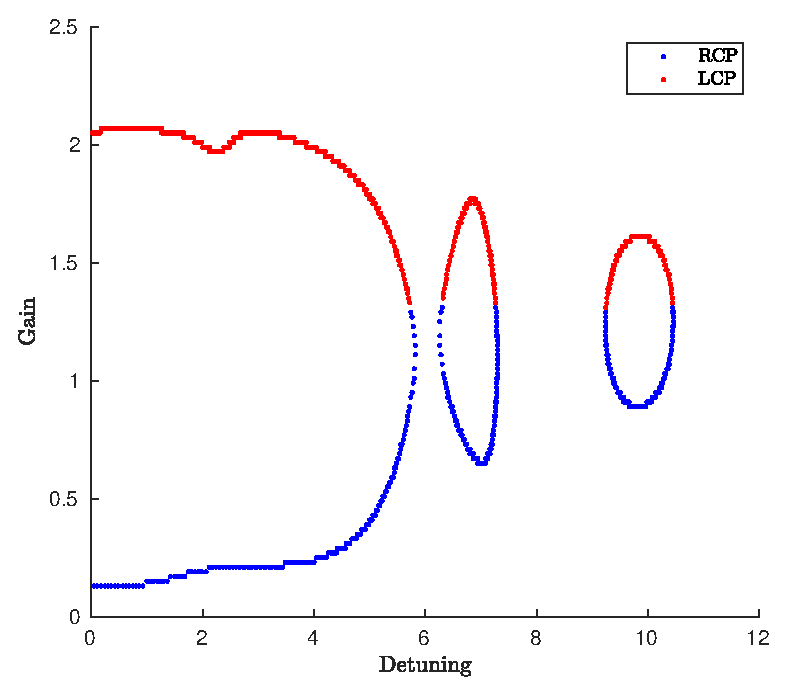
\includegraphics[width=0.30\textwidth]{plots/defect/tuning}
	\caption[Tuning of defect cavity]{Tuning of defect cavity. Modes are identified according to their handedness (\protect\tikz[baseline=-0.5ex]{\protect\fill[color=red] (0,0) circle (1ex) ;} left-handed, \protect\tikz[baseline=-0.5ex]{\protect\fill[color=blue] (0,0) circle (1ex) ;} right-handed) for a range of defect angle of $[-\pi;\pi]$}
	\label{fig:defect_cavity:tuning}
\end{wrapfigure}

\begin{figure}
	\centering
	\begin{subfigure}{0.49\textwidth}
		\begin{subfigure}{\textwidth}
			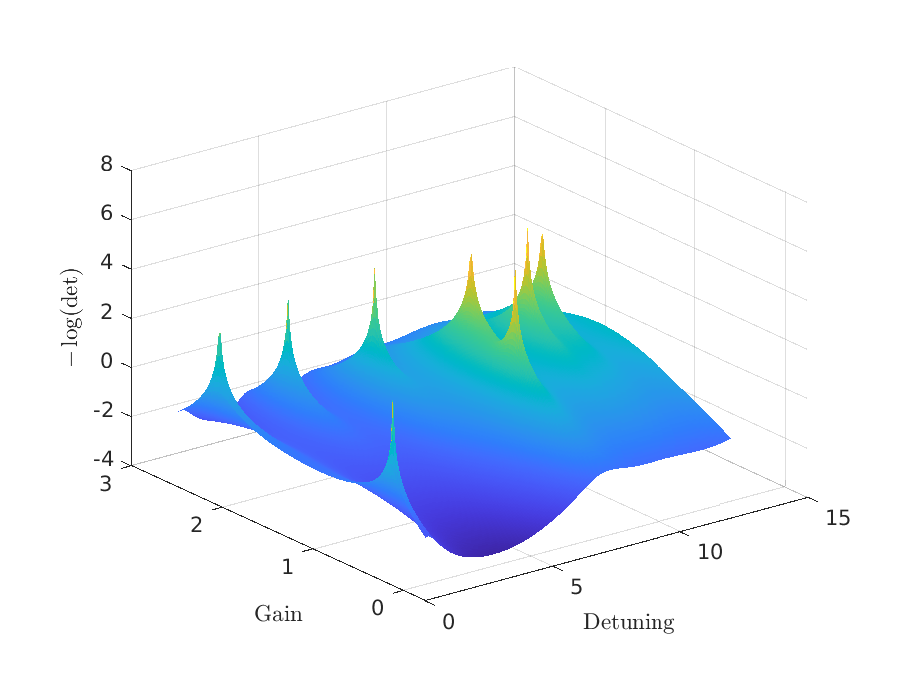
\includegraphics[width=\textwidth]{plots/defect/surface_oseen}
			\caption{}
			\label{fig:defect_cavity:oseen_surf}
		\end{subfigure}
		\begin{subfigure}{\textwidth}
			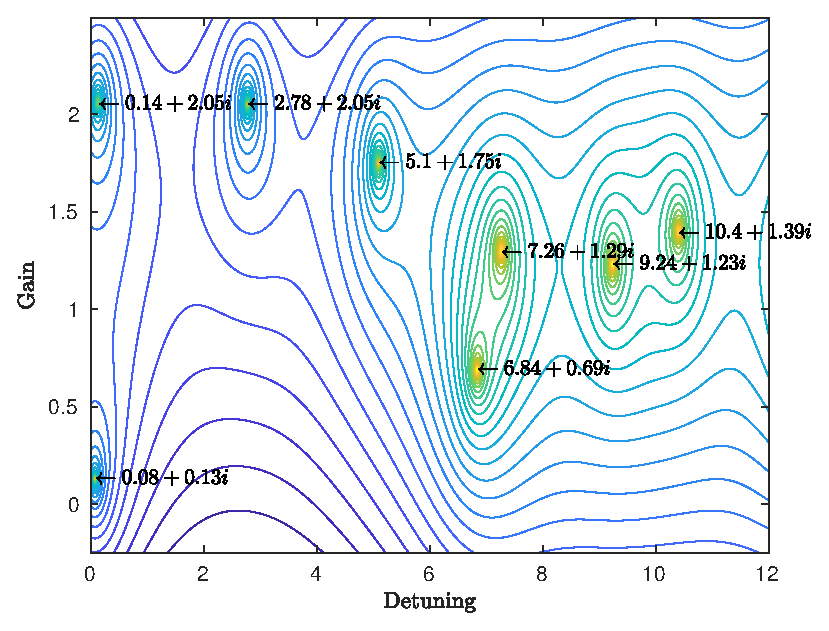
\includegraphics[width=\textwidth]{plots/defect/contour_oseen}
			\caption{}
			\label{fig:defect_cavity:oseen_contour}
		\end{subfigure}
		\begin{subfigure}{\textwidth}
			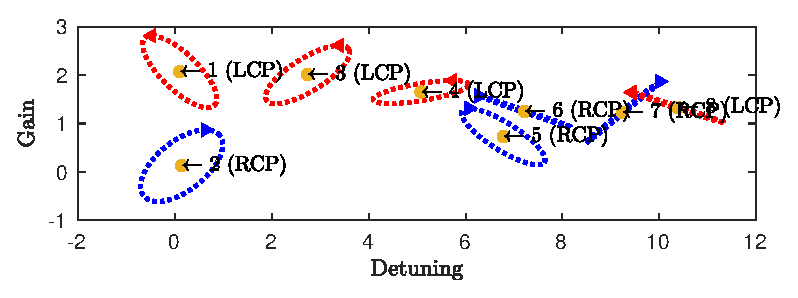
\includegraphics[width=\textwidth]{plots/defect/modes_found}
			\caption{}
			\label{fig:defect_cavity:modes_found}
		\end{subfigure}
	\end{subfigure}
	\begin{subfigure}{0.49\textwidth}
		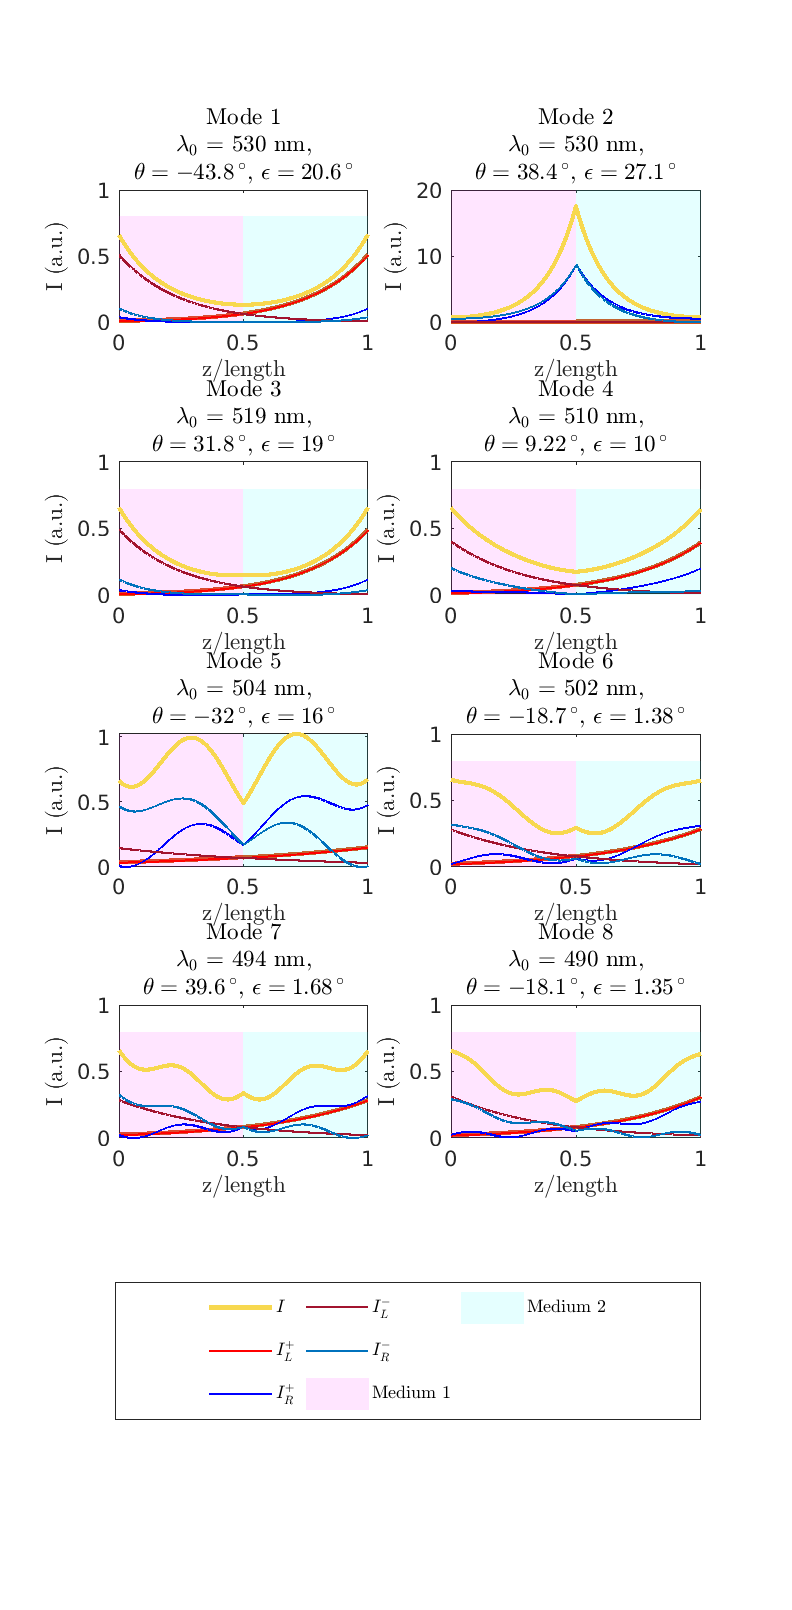
\includegraphics[width=\textwidth]{plots/defect/intensity_distribution}
		\caption{}
		\label{fig:defect_cavity:intensity_distribution}
	\end{subfigure}
	\caption[Comparison between methods for modeling a defect cavity.]{Analysis of the defect cavity. \ref{fig:defect_cavity:oseen_surf} shows the logarithm of the invert of the determinant of $\bm{M_{22}}$. \ref{fig:defect_cavity:oseen_contour} is the corresponding contour plot where the lasing modes have been identified. \ref{fig:defect_cavity:modes_found} Labeled modes found with the developed CWT and corresponding output ellipses in medium 1. \ref{fig:defect_cavity:intensity_distribution} Intensity distribution in the cavity for the modes in \ref{fig:defect_cavity:modes_found}. The intensity distribution yielded by exact theory is close to the approximate result and is given in figure \ref{fig:defect_intensity_appendix} in appendix \ref{chap:intensities}.}
	\label{fig:defect_cavity:surf}
\end{figure}

\subsection{Conclusion on the cavity with a defect}
	
This geometry does not produce pure circularly-polarised light. However it allows for interesting features such as highly selective band filter and fine laser tuning. The benefits of this cavity could be adapted in future designs in conjunction with a design allowing the output of purer circular modes.
\section{Hybrid cavity}

The third design simulated was a hybrid cavity consisting of a right-handed chiral gain medium placed between two left-handed chiral media acting as reflectors for left-circularly polarised light reflectors. The design is schematised in figure \ref{fig:hybrid}.

The lasing action of the cavity is simulated using the same method as before with the parameters given in table \ref{tab:hybrid_cavity:simulation}. Losses were added in the reflectors because otherwise zero-gain modes can be found. This makes sense mathematically because that means such modes are able to perform a round-trip in the cavity without being altered, but does not correspond to any physical reality as mirrors are necessary slightly lossy. Figure \ref{fig:hybrid_cavity:mycwt_surf} shows the lasing coefficient found with approximate theory (the result with exact theory was very close and thus is not shown). The corresponding output modes are then calculated for both method, and the intensity distributions are plotted in figure \ref{fig:hybrid_cavity:modes}.

The first thing to be noted is that this geometry produces very pure left or right circularly polarised modes. The second thing is that mode 1 requires left-handed light coming from the outside of the cavity. This is attributed to an imprecise localisation of this mode. The three displayed modes illustrate the dynamics at play in the cavity leading to the two possible output handedness. First, for left-handed output polarisations, light is not reflected by right-handed medium and travels in left-handed media, leading to chirality-preserving reflections schematised in figure \ref{fig:hybrid:mechanism_lh}. Then, for right-handed modes, the cavity acts as a simple cavity\cite{topf_modes_2014} with index-matched media at the interfaces, thus providing pure right-handed circularly polarised output as there are no Fabry-Pérot modes. This dynamic is  shown in figure \ref{fig:hybrid:mechanism_rh} and explains mode 3 in figure \ref{fig:hybrid_cavity:modes}.


\begin{table}
	\centering
	\begin{tabulary}{\linewidth}{LCC}
		\hline
		\hline
		Structural period of the chiral medium & $L_p$ & 300 nm \\
		Length of the left-handed chiral media & $L_L$ & $40\times L_p$ \\
		Length of the right-handed chiral media & $L_R$ & $20\times L_p$ \\
		Refractive index of the surrounding media & $n_1=n_2$ & 1 \\
		Average refractive index of the chiral media (Re) & $\Re{\bar{n}_{L,R}}$ & 1.7690 \\
		Average refractive index of the left-handed chiral media (Im) & $\Im{\bar{n}_L}$ & 0.02 \\
		Detuning range & $\mathrm{Re}(\delta k L_R / 2)$ & $[0,6]$ \\
		Gain range & $-\mathrm{Im}(\delta k L_R / 2)$ & $[0,3]$ \\
		Coupling constant & $\kappa_{L,R}$ & $4/L_{L,R}$\\
		\hline
		\hline
	\end{tabulary}
	\caption[Parameters for the cavity with a defect]{Parameters used for simulation.}
	\label{tab:hybrid_cavity:simulation}
\end{table}


\begin{figure}
	\centering
	\begin{subfigure}{0.48\linewidth}
		\begin{tikzpicture}
		\fill[red!20] (-1.5,1.2) -- (0,1.2) -- (0,-0.5) -- (-1.5,-0.5) -- cycle;
		\fill[red!20] (2,1.2) -- (3.5,1.2) -- (3.5,-0.5) -- (2,-0.5) -- cycle;
		\fill[cyan!20] (0,1.2) -- (2,1.2) -- (2,-0.5) -- (0,-0.5) -- cycle;
		\draw[red!80] (-0.75,1.2)node [above] {LHM} ;
		\draw[red!80] (2.75,1.2)node [above] {LHM} ;
		\draw[cyan!80] (1,1.2)node [above] {RHM} ;
		
		\draw[->, thick] (-0.5,0.75) -- node[above] {$L$} (2.5,0.75) arc  (90:-90:0.25) -- node[above] {$L$} (-0.5,0.25) arc (90:270:0.25) -- (0.5,-0.25) node[right] {$L$};
		\draw[decoration={brace,mirror,raise=1.5pt},decorate] (0,-0.5) -- node[below=2pt] {Gain medium} (2,-0.5);
		
		\fill[red] (3.75,0.5) -- (4,0.5) -- (4,0.6) -- (4.2,0.4) -- (4,0.2) -- (4,0.3) -- (3.75,0.3) -- cycle;
		\node[above right] at (3.5,0.6) {Out};
		\node[below right] at (3.5,0.25) {(LCP)};			
		
		\fill[red] (-1.75,0.5) -- (-2,0.5) -- (-2,0.6) -- (-2.2,0.4) -- (-2,0.2) -- (-2,0.3) -- (-1.75,0.3) -- cycle;
		\node[above left] at (-1.5,0.6) {Out};
		\node[below left] at (-1.5,0.25) {(LCP)};
		
		\end{tikzpicture}
		\caption{}
		\label{fig:hybrid:mechanism_lh}
	\end{subfigure}
	\begin{subfigure}{0.48\linewidth}
		\begin{tikzpicture}
		\fill[red!20] (-1.5,1.2) -- (0,1.2) -- (0,-0.5) -- (-1.5,-0.5) -- cycle;
		\fill[red!20] (2,1.2) -- (3.5,1.2) -- (3.5,-0.5) -- (2,-0.5) -- cycle;
		\fill[cyan!20] (0,1.2) -- (2,1.2) -- (2,-0.5) -- (0,-0.5) -- cycle;
		\draw[red!80] (-0.75,1.2)node [above] {LHM} ;
		\draw[red!80] (2.75,1.2)node [above] {LHM} ;
		\draw[cyan!80] (1,1.2)node [above] {RHM} ;
		
		\draw[->, thick] (0.5,0.75) -- node[above] {$R$} (1.5,0.75) arc  (90:-90:0.25) -- node[above] {$R$} (0.5,0.25) arc (90:270:0.25) -- node[right] {$R$} (0.75,-0.25);
		\draw[decoration={brace,mirror,raise=1.5pt},decorate] (0,-0.5) -- node[below=2pt] {Gain medium} (2,-0.5);
		
		\fill[red] (3.75,0.5) -- (4,0.5) -- (4,0.6) -- (4.2,0.4) -- (4,0.2) -- (4,0.3) -- (3.75,0.3) -- cycle;
		\node[above right] at (3.5,0.6) {Out};
		\node[below right] at (3.5,0.25) {(RCP)};
		
		
		\fill[red] (-1.75,0.5) -- (-2,0.5) -- (-2,0.6) -- (-2.2,0.4) -- (-2,0.2) -- (-2,0.3) -- (-1.75,0.3) -- cycle;
		\node[above left] at (-1.5,0.6) {Out};
		\node[below left] at (-1.5,0.25) {(RCP)};
		
		\end{tikzpicture}
		\caption{}
		\label{fig:hybrid:mechanism_rh}
	\end{subfigure}
	\caption[Mechanisms leading to laser action in an hybrid cavity]{Mechanisms leading to laser action in an hybrid cavity. \ref{fig:hybrid:mechanism_lh} Reflections of left-handed light on the reflectors. \ref{fig:hybrid:mechanism_rh} Reflections of right-handed light inside the gain medium.}
	
\end{figure}

\begin{figure}
	\centering
	\begin{subfigure}{0.49\textwidth}
		\begin{subfigure}{\textwidth}
			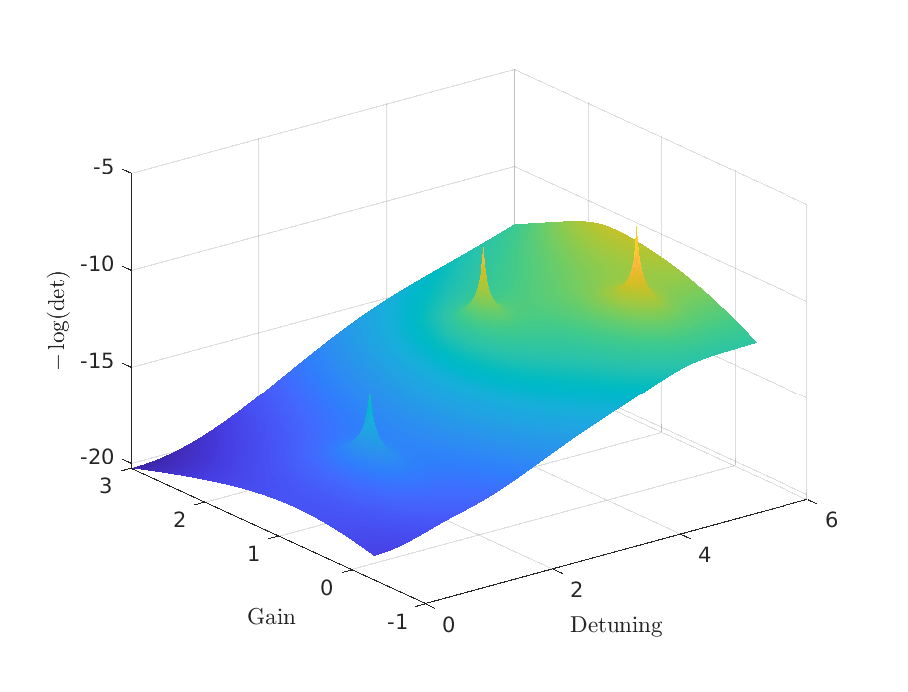
\includegraphics[width=\textwidth]{plots/hybrid/surface}
			\caption{}
			\label{fig:hybrid_cavity:mycwt_surf}
		\end{subfigure}	
		\begin{subfigure}{\textwidth}
			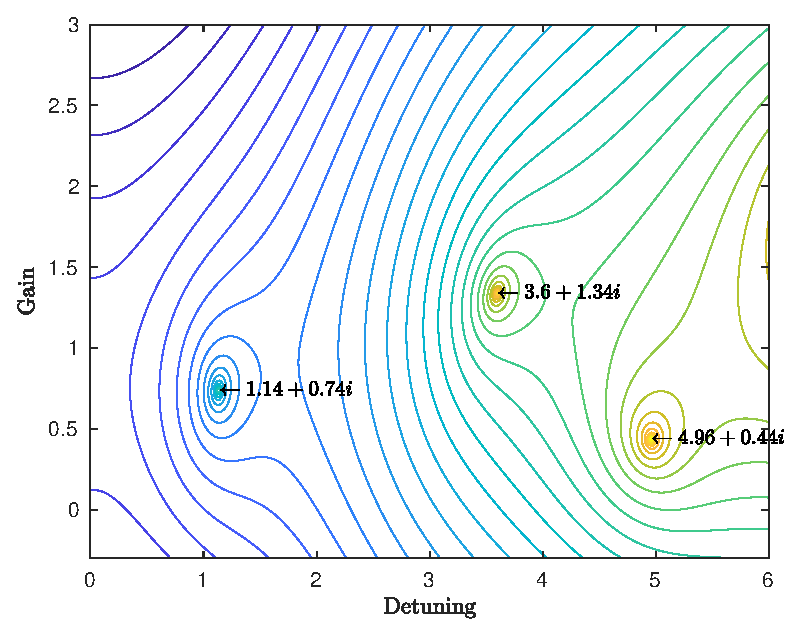
\includegraphics[width=\textwidth]{plots/hybrid/contour}
			\caption{}
			\label{fig:hybrid_cavity:mycwt_contour}
		\end{subfigure}
	\end{subfigure}
	\begin{subfigure}{0.49\textwidth}
		\begin{subfigure}{\textwidth}
			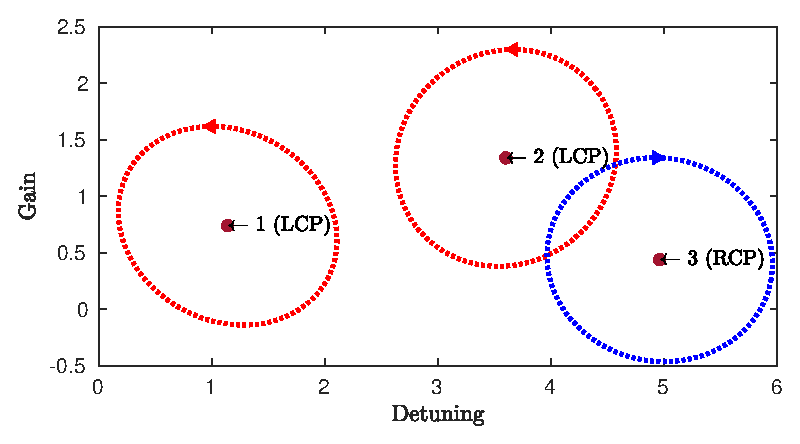
\includegraphics[width=\textwidth]{plots/hybrid/modes_found}
			\caption{Developed CWT}
			\label{fig:hybrid_cavity:modes_found}
		\end{subfigure}
		\begin{subfigure}{\textwidth}
			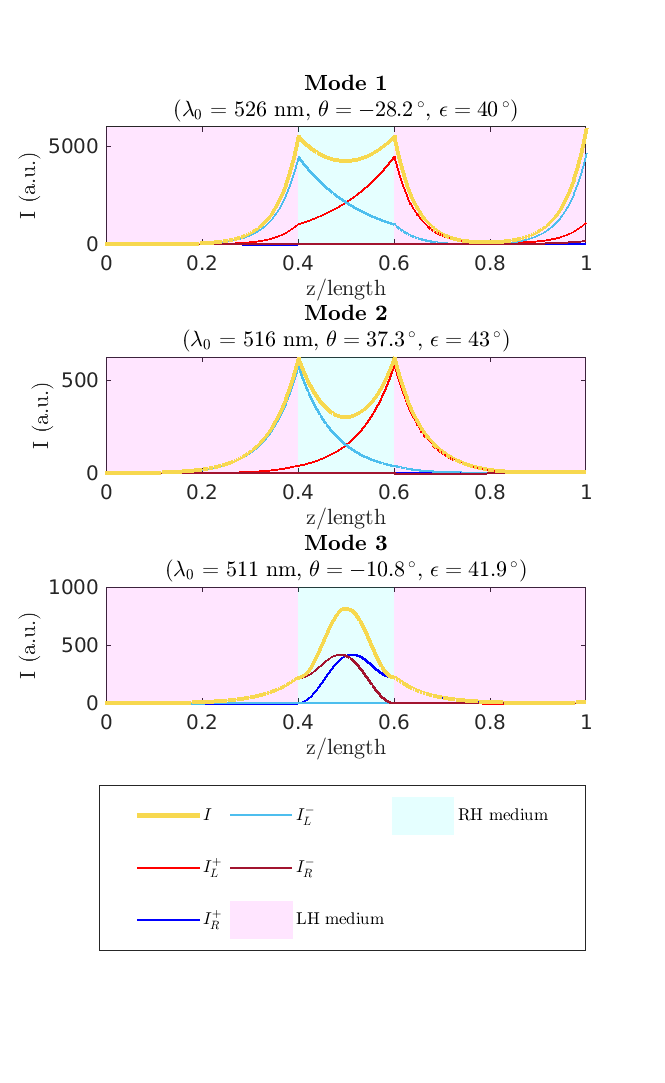
\includegraphics[width=\textwidth]{plots/hybrid/intensity_distribution}
			\caption{}
			\label{fig:hybrid_cavity:intensity_distribution}
		\end{subfigure}
	\end{subfigure}
	\caption[Analysis of hybrid cavity]{Analysis of hybrid cavity. \ref{fig:hybrid_cavity:mycwt_surf} shows the logarithm of the invert of the determinant of $\bm{M_{22}}$. \ref{fig:hybrid_cavity:mycwt_contour} is the corresponding contour plot where the lasing modes have been identified. \ref{fig:hybrid_cavity:modes_found} Labelled modes found with the developed CWT and corresponding output ellipses in medium 1. \ref{fig:hybrid_cavity:intensity_distribution} Intensity distribution in the cavity for the modes in \ref{fig:hybrid_cavity:modes_found}. The results yielded by exact theory are similar and are presented in figure \ref{fig:hybrid_intensity_appendix} in appendix \ref{chap:intensities}.}
	\label{fig:hybrid_cavity:modes}
\end{figure}

\subsection{Conclusion on hybrid cavity}

The hybrid cavity geometry solves the issue of impurities present in the output of a simple cavity and a defect cavity. This is because the hybrid geometry simplifies the dynamics of reflections in the cavity, removing the chirality-reversing reflections due to unmatched index interfaces. The left-handed modes require higher gain, because of the losses in left-handed media where the reflections occur.
\clearpage
\section{Hybrid defect cavity}

The last geometry simulated is a hybrid cavity with a defect in the centre. The goal is to have the benefits of both the defect cavity, \textit{i.e.} the tunability of the cavity, and hybrid cavity, \textit{i.e.} high purity of output modes. The cavity design is shown in figure \ref{fig:hybrid_defect}.

Figure \ref{fig:hybrid_defect:analysis} shows an analysis of the cavity laser action for a defect of $\frac{\pi}{2}$. As expected this geometry presents the features of both defect and hybrid cavities. Mode 1 in figure \ref{fig:hybrid_defect:intensity} presents strong confinement within the defect while the hybrid structure ensures fairly pure circular polarisation output : the worst polarisation is mode 1 with $\epsilon=37^\circ$.

\begin{figure}
	\centering
	\begin{subfigure}{0.48\linewidth}
		\begin{subfigure}{\linewidth}
			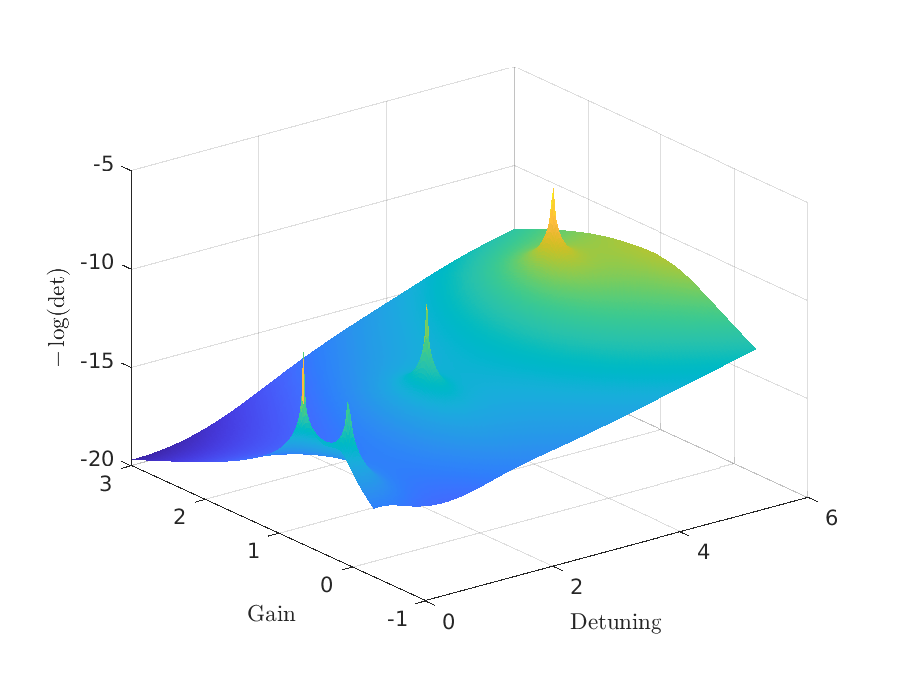
\includegraphics[width=\linewidth]{plots/hybrid_defect/pi_2/surface}
			\caption{}
			\label{fig:hybrid_defect:surf}
		\end{subfigure}
		\begin{subfigure}{\linewidth}
			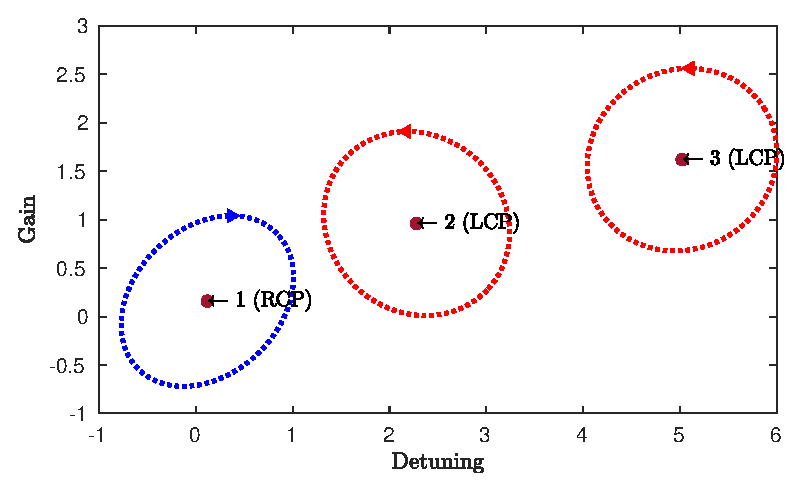
\includegraphics[width=\linewidth]{plots/hybrid_defect/pi_2/modes_found}
			\caption{}
			\label{fig:hybrid_defect:modes}
		\end{subfigure}
	\end{subfigure}
	\begin{subfigure}{0.48\linewidth}
		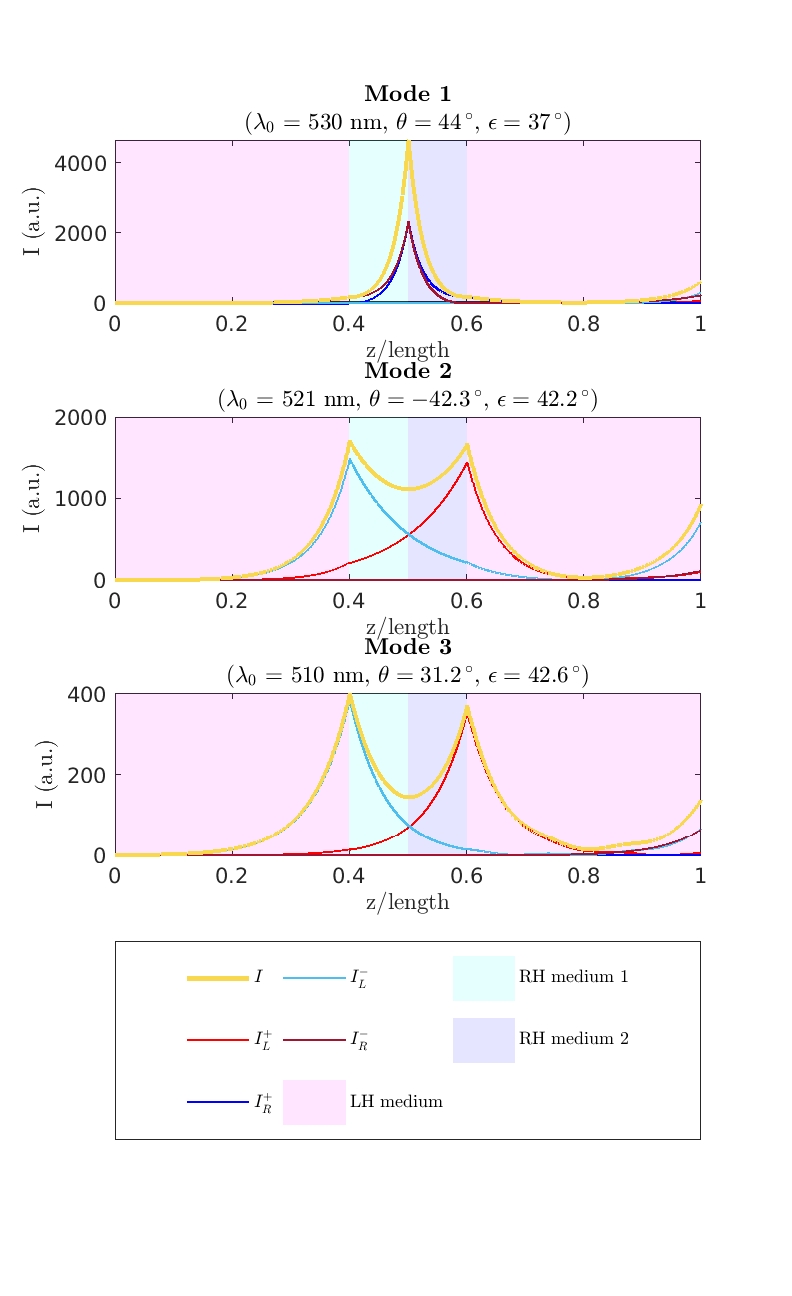
\includegraphics[width=\linewidth]{plots/hybrid_defect/pi_2/intensity_distribution}
		\caption{}
		\label{fig:hybrid_defect:intensity}
	\end{subfigure}
	\caption[Analysis of hybrid defect cavity]{Analysis of laser action for a $\frac{\pi}{2}$ defect. \ref{fig:hybrid_defect:surf} Reciprocal of the determinant of $\bm{M_{22}}$. \ref{fig:hybrid_defect:modes} Identification of output modes. \ref{fig:hybrid_defect:intensity} Intensity distribution in the cavity for found modes. The results yielded by exact theory are available in figure \ref{fig:hybrid_defect_pi2_intensity_appendix} in appendix \ref{chap:intensities}.}
	\label{fig:hybrid_defect:analysis}
\end{figure}

To study the tunability of the cavity, its output is examined over a range of defects $\psi$ going from $-\pi$ to $\pi$. The lasing loci are presented in figure \ref{fig:hybrid_defect:tuning}, showing that there seems to be a corresponding gain and defect angle allowing laser action for every detuning in the range scanned. 

Figures \ref{fig:hybrid_defect:purity}, \ref{fig:hybrid_defect:purity_lh} and \ref{fig:hybrid_defect:purity_rh} provide the distribution of output $\epsilon$ for respectively the 613 modes found, the 465 left-handed modes found and the 148 right-handed modes found. This shows the average output $\epsilon$ is $38.66^\circ$, with a standard deviation of $3.9^\circ$. Thus, the output modes are almost pure circularly polarised. Figure \ref{fig:hybrid_defect:purity_3D} shows the distribution of modes purity against detuning and gain. Figure \ref{fig:hybrid_defect:ellipses} show the corresponding ellipses for the extrema of the distribution of $\epsilon$.

\begin{figure}
	\centering
	\begin{subfigure}{.49\linewidth}
		\begin{subfigure}{\linewidth}
			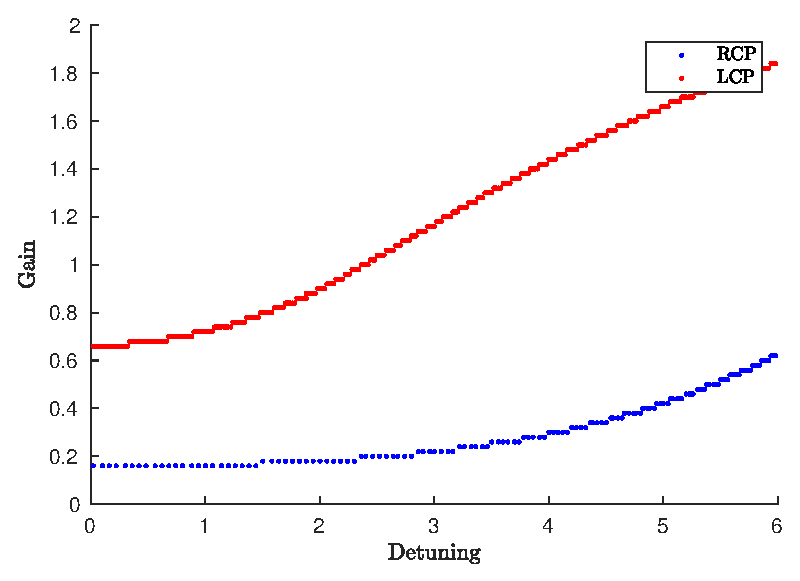
\includegraphics[width=\linewidth]{plots/hybrid_defect/tuning}
			\caption{}
			\label{fig:hybrid_defect:tuning}
		\end{subfigure}
		\begin{subfigure}{\linewidth}
			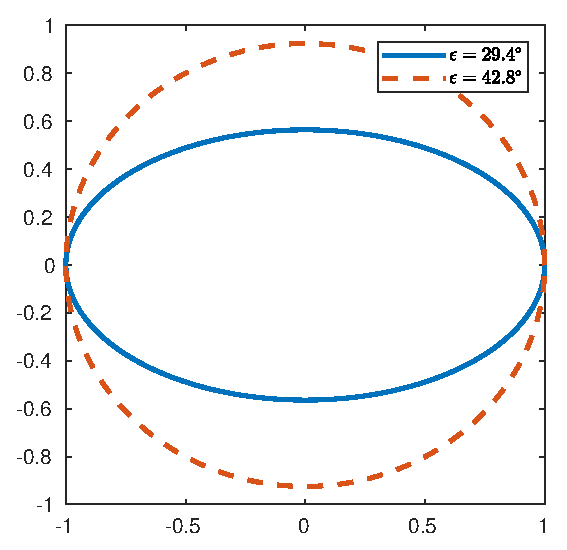
\includegraphics[width=\linewidth]{plots/hybrid_defect/ellipses}
			\caption{}
			\label{fig:hybrid_defect:ellipses}
		\end{subfigure}
		\begin{subfigure}{\linewidth}
			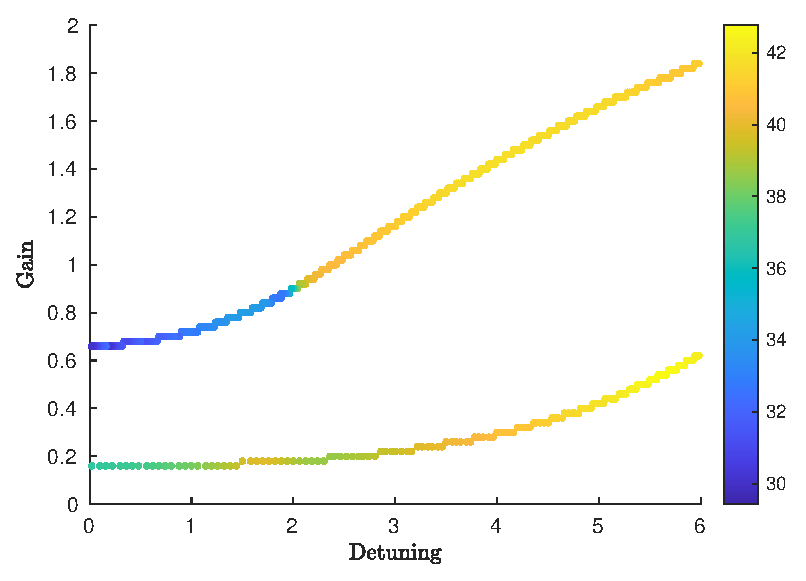
\includegraphics[width=\linewidth]{plots/hybrid_defect/purity_3D}
			\caption{}
			\label{fig:hybrid_defect:purity_3D}
		\end{subfigure}
	\end{subfigure}
	\begin{subfigure}{0.49\linewidth}
		\begin{subfigure}{\linewidth}
			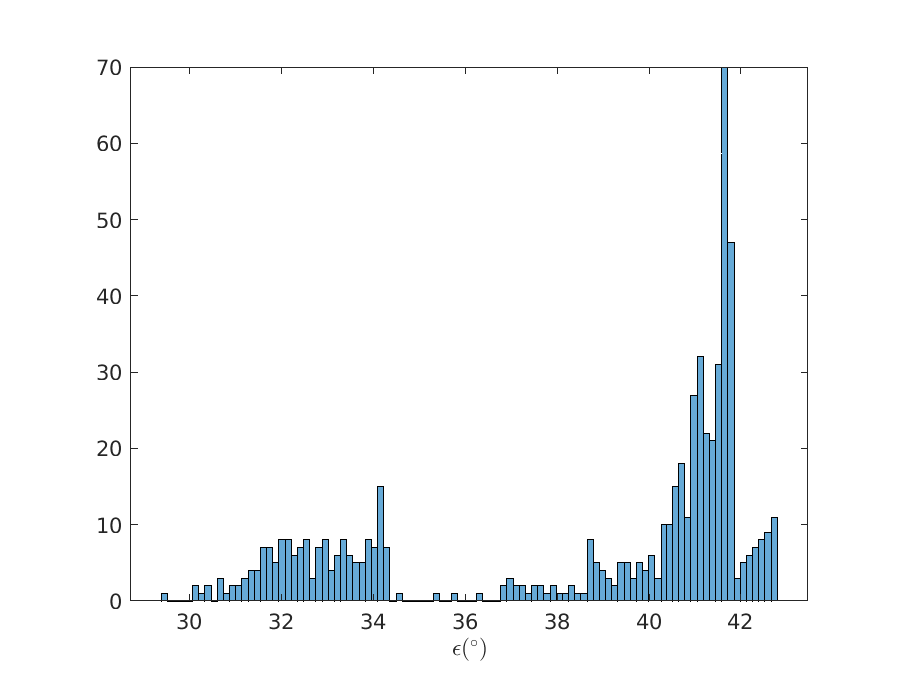
\includegraphics[width=\linewidth]{plots/hybrid_defect/purity}
			\caption{}
			\label{fig:hybrid_defect:purity}
		\end{subfigure}
		\begin{subfigure}{\linewidth}
			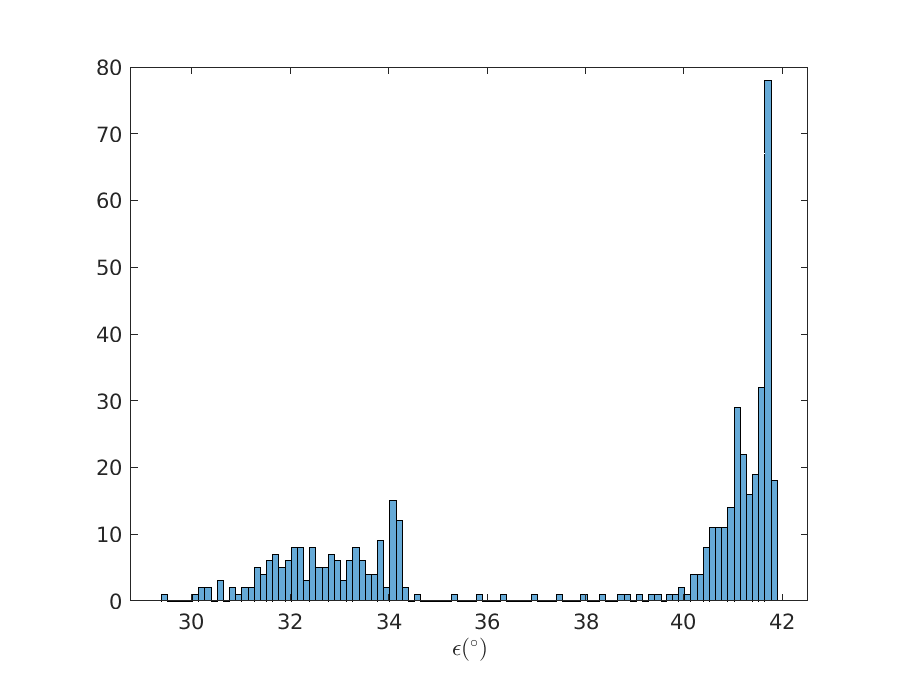
\includegraphics[width=\linewidth]{plots/hybrid_defect/purity_lh}
			\caption{}
			\label{fig:hybrid_defect:purity_lh}
		\end{subfigure}
		\begin{subfigure}{\linewidth}
			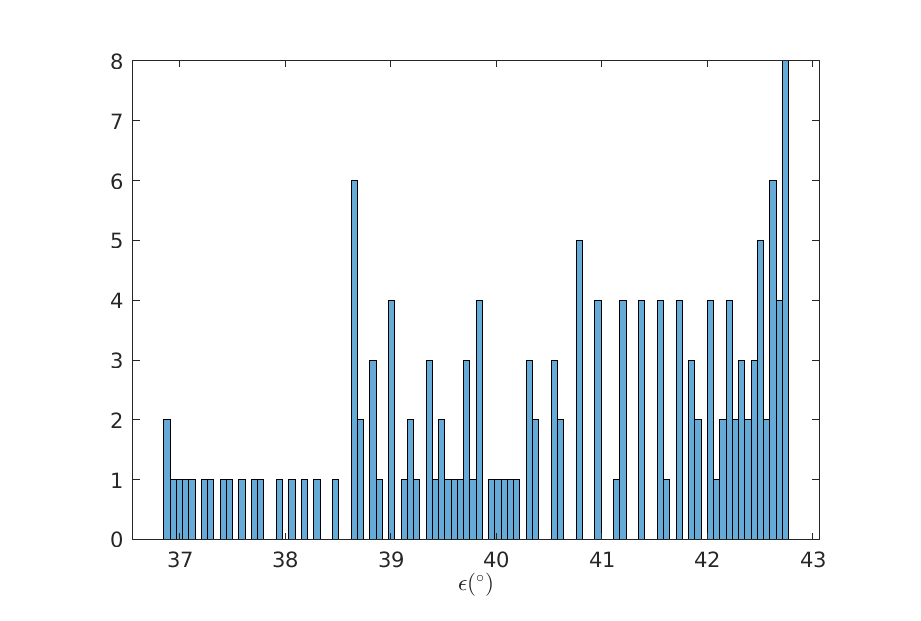
\includegraphics[width=\linewidth]{plots/hybrid_defect/purity_rh}
			\caption{}
			\label{fig:hybrid_defect:purity_rh}
		\end{subfigure}
	\end{subfigure}
	\caption[Scan through the possible defects of hybrid defect cavity]{Scan for a defect comprised in $[-\pi, \pi]$ radians. \ref{fig:hybrid_defect:tuning} Positions and handednesses of output modes. \ref{fig:hybrid_defect:ellipses} Output ellipses for the extrema of figure \ref{fig:hybrid_defect:purity}. \ref{fig:hybrid_defect:purity_3D} Distribution of $\epsilon$ for identified lasing modes. \ref{fig:hybrid_defect:purity} Distribution of output $\epsilon$ of the cavity. $\epsilon = 45^\circ$ corresponds to a perfect circle and $\epsilon=0^\circ$ to a linearly polarised output. \ref{fig:hybrid_defect:purity_lh} Distribution of output $\epsilon$ for left-handed polarisations. \ref{fig:hybrid_defect:purity_rh} Distribution of output $\epsilon$ for right-handed polarisations.}
\end{figure}

\subsection{Proposed explanation for the tunability of the cavity}

As shown in intensity distribution plots, the defect provides strong confinement of right-handed polarised light within it. Thus, this allows adjusting the effective optical length of the cavity for right-handed polarised light and, given the right gain, allows for lasing. A similar mechanism could explain tunability for left-handed polarised light. Indeed the two left-handed media also differ by a rotation corresponding to the defect. Thus, by adjusting the defect, it is possible to adjust the effective length of the cavity to a given detuning, providing laser action when the gain is suitably adjusted.

\subsection{Conclusion on hybrid defect cavity}
This design manages to combine the advantages of both defect and hybrid cavities. Indeed, it seems that it allows producing relatively pure circularly polarised modes for any detuning of the cavity, given the correct angle of defect and gain. Furthermore, for a given detuning, it seems possible to switch between left and right circularly polarised light by changing the defect and gain, which makes such a laser highly versatile. A more detailed study, perhaps analytical, aiming to give a direct way to estimate gain and angle of defect given a cavity detuning would be a great addition here.
\chapter{Conclusion}
Exact and coupled-waves theory are extensively presented and coupled-waves theory is extended to include rotations along propagation axis, left-handed media and interfaces. 

Previous results are successfully reproduced and new designs are implemented. First, cavity with a rotational design allows finely tuning the cavity to produce laser output for many cavity detunings. Then, hybrid cavity composed of a chiral gain medium surrounded by two chiral reflectors of opposite handedness allows producing highly pure circularly polarised outputs. Combining both techniques allows taking the best of both worlds and leads to the hybrid chiral defect cavity, a highly tunable circularly polarised laser source. 

The final design presented could very well be at the heart of the design of new kinds of 3D projectors when implemented with liquid-crystals media in laser matrices. This is could also be used to implement broadband characterisation devices based on ellipsometry. 

The coupled-waves theory could also be extended even further, allowing to simulate cavities with physical beams. Indeed, this study focuses on plane-waves that propagate along the axis of the birefringence helix. However, since the effective refractive index depends on the angle of propagation, physical beams such as Gaussian beams would effectively experience different refractive index depending on the position in the $(x,y)$ plane for a given position $z$. This could lead to interesting effects similar to self-focusing in non-linear optics\cites{poy_chirality-enhanced_2020}{shishkov_polarization_2020}.
\printbibliography
\appendix
\chapter{Source code}
\label{chap:sourcecode}

The source code used to produce the figures of this report is hosted at \url{https://github.com/Klafyvel/Hybrid-Chiral-Lasers}. This appendix describes the different files present.

\paragraph{Utilitaries}

\begin{description}
	\item[ellipse.m] Calculate the points belonging to an ellipse given the parameters $\epsilon$, the rotation $\theta$, the position $(x_0, y_0)$, the semi-major axis $a$ and a number of points $n$.
	\item[find\_max.m] Find the local maxima of a 2D array. The local maxima must be a maximum in a rectangle of size \verb|radx|$\times$\verb|rady|.
	\item[find\_modes.m] Find the output modes corresponding to the cavities at \verb|row,col|. Outputs \verb|R, theta, epsilon, lcp, modes|, the radius, rotation, parameter, a boolean which is \verb|true| for left-handed polarisations and the corresponding electrical field.
	\item[partial\_inverse.m] Calculate the partial inverse of a $4\times4$ matrix.
	\item[plot\_ellipse.m] Plot the output polarisation ellipses.
	\item[rotation.m] Calculate a rotation matrix.
	\item[savefig.m] Smartly save a figure, without overriding older plots.
	\item[reflection\_cwt.m] Calculate the reflection matrix associated with a transfer matrix in circular basis.
	\item[reflection\_oseen.m] Calculate the reflection matrix associated with a matrix in electro-magnetic basis, given the refractive indices of surrounding media.
	\item[transmission\_cwt.m] Calculate the transmission matrix associated with a transfer matrix in circular basis.
	\item[transmission\_oseen.m] Calculate the transmission matrix associated with a matrix in electro-magnetic basis, given the refractive indices of surrounding media.
\end{description}

\paragraph{Transfer matrices}

\begin{description}
	\item[oseen.m] Transfer matrix for the Oseen method, given $p, \epsilon_a, \epsilon_b, \psi, L, k_0$ in electromagnetic basis.
	\item[cwt.m] Transfer matrix for coupled-waves theory given $p, \epsilon_a, \epsilon_b, \psi, L, k_0$ and \verb|lhm| the handedness.
	\item[cwt\_from\_reduced\_variables.m] Same as above, but given $p, \psi, L, k, \kappa, \delta k$ and \verb|lhm|.
	\item[cwt\_convenient\_variables.m] Calculate reduced parameters from parameters of \verb|cwt.m|.
	\item[cwt\_circular\_to\_emag\_basis.m] Calculate the matrix to switch from circular to electromagnetic matrix given the parameters of \verb|cwt.m|.
	\item[cwt\_circular\_to\_emag\_basis\_from\_reduced\_variables.m] Same as above but with reduced parameters.
	\item[interface\_chiral\_same\_handedness.m] Matrix for the interface between two media of same handedness.
	\item[interface\_chiral\_same\_handedness\_from\_reduced\_variables.m] Same as above, with reduced variables.
	\item[interface\_chiral\_to\_isotrope.m] Matrix for the interface between chiral media and isotropic media.
	\item[interface\_chiral\_to\_isotrope\_from\_reduced\_variables.m] Same as above, with reduced variables.
	\item[interface\_left\_to\_right.m] Matrix for the interface from a left-handed media to a right-handed one.
	\item[interface\_left\_to\_right\_from\_reduced\_variables.m] Same as above, with reduced variables.
\end{description}

\paragraph{Reflectivities}

\begin{description}
	\item[simple\_cavity\_transmission.m] Transmission coefficients for the simple cavity.
	\item[check\_energy\_conservation.m] Calculate energy conservation coefficients for the simple cavity.
	\item[narrow\_band.m] Transmission coefficients for the cavity with a defect.
\end{description}

\paragraph{Cavities}

\begin{description}
	\item[simple\_cavity.m] Reproduce the cavity described by \textcite{topf_modes_2014} using various methods.
	\item[defect\_lasing.m] Cavity with a defect.
	\item[defect\_tuning.m] Scan through the possible defect angles of the simple cavity. This code takes more than an hour to run on my computer.
	\item[hybrid\_cavity.m] Hybrid cavity.
	\item[hybrid\_defect\_cavity.m] Hybrid cavity with a defect.
	\item[hybrid\_defect\_tuning.m] Scan through the possible defect angles of the hybrid cavity. This code takes more than an hour to run on my computer.
\end{description}
\chapter{Reflectivities}
\label{chap:reflectivities}

\begin{figure}
	\centering
	\begin{subfigure}{0.49\linewidth}
		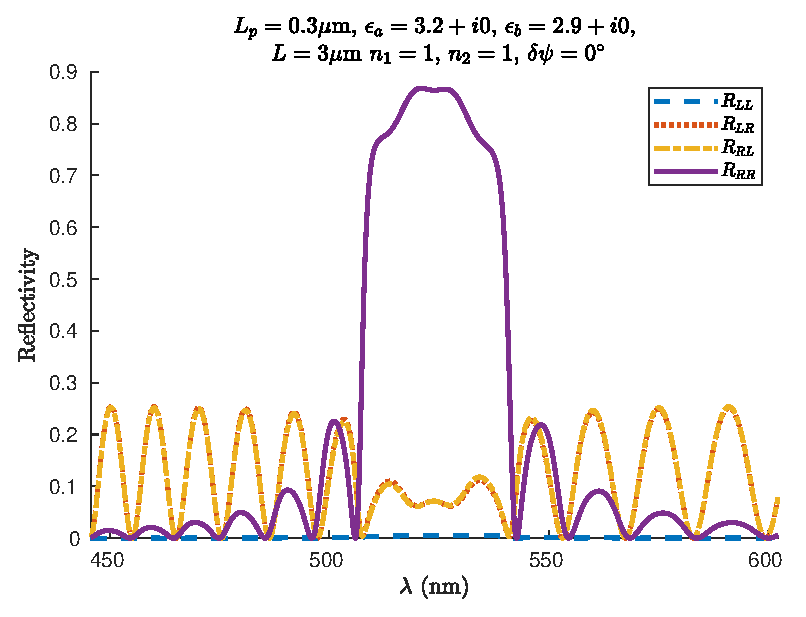
\includegraphics[width=\linewidth]{plots/defect/no_defect/cwt_reflection}
		\caption{}
	\end{subfigure}
	\begin{subfigure}{0.49\linewidth}
		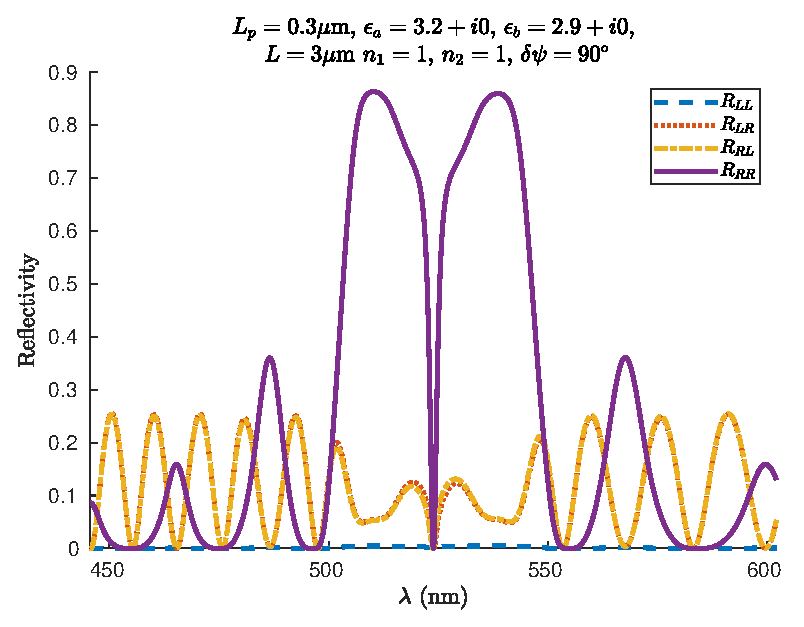
\includegraphics[width=\linewidth]{plots/defect/reflectivity/cwt_reflection}
		\caption{}
	\end{subfigure}
	\begin{subfigure}{0.49\linewidth}
		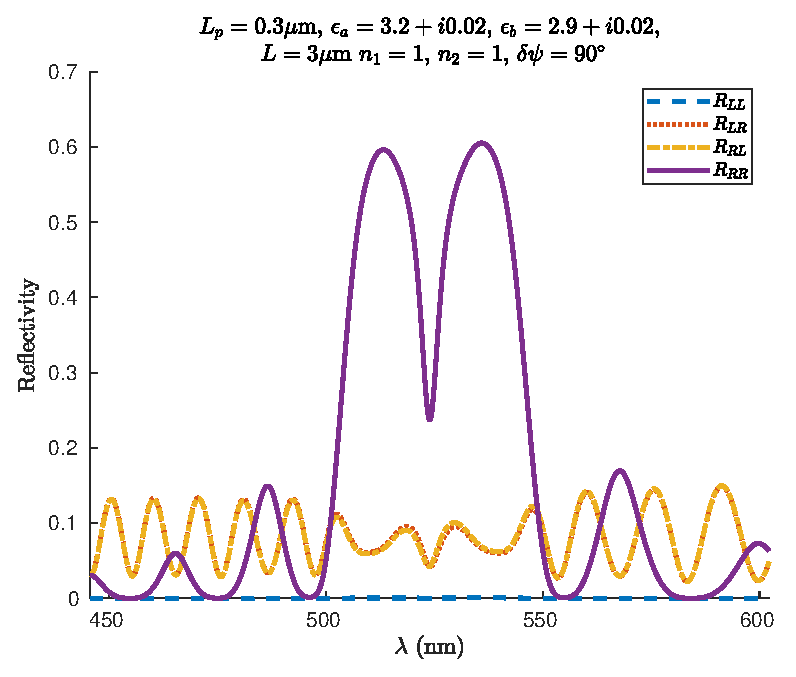
\includegraphics[width=\linewidth]{plots/defect/reflectivity_losses/cwt_reflection}
		\caption{}
	\end{subfigure}
	\begin{subfigure}{0.49\linewidth}
		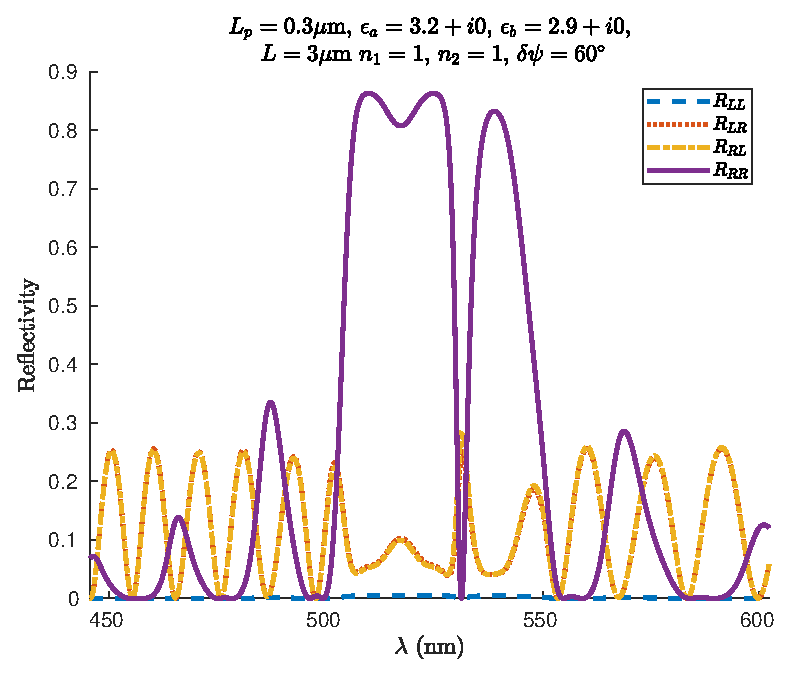
\includegraphics[width=\linewidth]{plots/defect/reflectivity_other_defect/cwt_reflection}
		\caption{}
	\end{subfigure}
	\caption[Reflectivity of the narrow-band filter]{Reflectivities of narrow-band filter with coupled wave theory}
	\label{fig:reflectivities_narrow_appendix}
\end{figure}

\begin{figure}
	\centering
	\begin{subfigure}{0.49\linewidth}
		\includegraphics[width=\linewidth]{plots/defect/no_defect/comparison_reflection}
		\caption{}
	\end{subfigure}
	\begin{subfigure}{0.49\linewidth}
		\includegraphics[width=\linewidth]{plots/defect/reflectivity/comparison_reflection}
		\caption{}
	\end{subfigure}
	\begin{subfigure}{0.49\linewidth}
		\includegraphics[width=\linewidth]{plots/defect/reflectivity_losses/comparison_reflection}
		\caption{}
	\end{subfigure}
	\begin{subfigure}{0.49\linewidth}
		\includegraphics[width=\linewidth]{plots/defect/reflectivity_other_defect/comparison_reflection}
		\caption{}
	\end{subfigure}
	\caption[Comparison of reflectivity of the narrow-band filter]{Comparison of reflectivities of narrow-band filter with coupled wave theory and exact theory}
	\label{fig:reflectivities_narrow_appendix_comp}
\end{figure}
\chapter{Transmitivities}
\label{chap:transmitivities}

\begin{figure}
	\centering
	\begin{subfigure}{0.49\linewidth}
		\includegraphics[width=\linewidth]{plots/defect/no_defect/oseen_transmission}
		\caption{}
	\end{subfigure}
	\begin{subfigure}{0.49\linewidth}
		\includegraphics[width=\linewidth]{plots/defect/reflectivity/oseen_transmission}
		\caption{}
	\end{subfigure}
	\begin{subfigure}{0.49\linewidth}
		\includegraphics[width=\linewidth]{plots/defect/reflectivity_losses/oseen_transmission}
		\caption{}
	\end{subfigure}
	\begin{subfigure}{0.49\linewidth}
		\includegraphics[width=\linewidth]{plots/defect/reflectivity_other_defect/oseen_transmission}
		\caption{}
	\end{subfigure}
	\caption[Transmitivities of the narrow-band filter, exact theory]{Transmitivities of narrow-band filter with exact theory}
	\label{fig:transitivities_narrow_appendix_exact}
\end{figure}

\begin{figure}
	\centering
	\begin{subfigure}{0.49\linewidth}
		\includegraphics[width=\linewidth]{plots/defect/no_defect/cwt_transmission}
		\caption{}
	\end{subfigure}
	\begin{subfigure}{0.49\linewidth}
		\includegraphics[width=\linewidth]{plots/defect/reflectivity/cwt_transmission}
		\caption{}
	\end{subfigure}
	\begin{subfigure}{0.49\linewidth}
		\includegraphics[width=\linewidth]{plots/defect/reflectivity_losses/cwt_transmission}
		\caption{}
	\end{subfigure}
	\begin{subfigure}{0.49\linewidth}
		\includegraphics[width=\linewidth]{plots/defect/reflectivity_other_defect/cwt_transmission}
		\caption{}
	\end{subfigure}
	\caption[Transmitivities of the narrow-band filter]{Transmitivities of narrow-band filter with coupled wave theory}
	\label{fig:transitivities_narrow_appendix}
\end{figure}

\begin{figure}
	\centering
	\begin{subfigure}{0.49\linewidth}
		\includegraphics[width=\linewidth]{plots/defect/no_defect/comparison_transmission}
		\caption{}
	\end{subfigure}
	\begin{subfigure}{0.49\linewidth}
		\includegraphics[width=\linewidth]{plots/defect/reflectivity/comparison_transmission}
		\caption{}
	\end{subfigure}
	\begin{subfigure}{0.49\linewidth}
		\includegraphics[width=\linewidth]{plots/defect/reflectivity_losses/comparison_transmission}
		\caption{}
	\end{subfigure}
	\begin{subfigure}{0.49\linewidth}
		\includegraphics[width=\linewidth]{plots/defect/reflectivity_other_defect/comparison_transmission}
		\caption{}
	\end{subfigure}
	\caption[Comparison of transmitivities of the narrow-band filter]{Comparison of transmitivities of narrow-band filter with coupled wave theory and exact theory}
	\label{fig:transmitivities_narrow_appendix_comp}
\end{figure}
\chapter{Intensity distributions}
\label{chap:intensities}

\begin{figure}
	\centering
	\begin{subfigure}{\linewidth}
		\includegraphics[width=\linewidth]{plots/defect/modes_found_oseen}
		\caption{}
	\end{subfigure}
	\begin{subfigure}{\linewidth}
		\includegraphics[width=\linewidth]{plots/defect/intensity_distribution_oseen}
		\caption{}
	\end{subfigure}
	\caption[Intensity distribution of defect cavity, exact theory]{Intensity distribution of defect cavity, exact theory}
	\label{fig:defect_intensity_appendix}
\end{figure}

\begin{figure}
	\centering
	\begin{subfigure}{\linewidth}
		\includegraphics[width=\linewidth]{plots/hybrid/modes_found_oseen}
		\caption{}
	\end{subfigure}
	\begin{subfigure}{\linewidth}
		\includegraphics[width=\linewidth]{plots/hybrid/intensity_distribution_oseen}
		\caption{}
	\end{subfigure}
	\caption[Intensity distribution of hybrid cavity, exact theory]{Intensity distribution of hybrid cavity, exact theory}
	\label{fig:hybrid_intensity_appendix}
\end{figure}

\begin{figure}
	\centering
	\begin{subfigure}{\linewidth}
		\includegraphics[width=\linewidth]{plots/hybrid_defect/pi_2/modes_found_oseen}
		\caption{}
	\end{subfigure}
	\begin{subfigure}{\linewidth}
		\includegraphics[width=\linewidth]{plots/hybrid_defect/pi_2/intensity_distribution_oseen}
		\caption{}
	\end{subfigure}
	\caption[Intensity distribution of hybrid defect cavity, defect of $\pi/2$, exact theory]{Intensity distribution of hybrid defect cavity, defect of $\pi/2$, exact theory}
	\label{fig:hybrid_defect_pi2_intensity_appendix}
\end{figure}

\end{document}
